\documentclass[fancyheaders,chapterformata]{thesis}
\raggedbottom  % causes excess space on pages to be moved to the bottom. Remove
               % to have excess space inserted between paragraphs instead.

\usepackage{times}
\usepackage{epsfig}
\usepackage[T1]{fontenc}
\usepackage[utf8]{inputenc}
% \usepackage{amsmath}
% \usepackage{amssymb}
% \usepackage{graphicx}
% \usepackage{graphics}
% \usepackage{array}
% \usepackage{url}
% \usepackage{algorithm}
% \usepackage{algorithmic}
% \usepackage{subfigure}
% \usepackage{color}
% Make text in figure legends singlespaced:
\usepackage[font=singlespacing]{caption}

% biblatex
\usepackage[style=apa,backend=biber,hyperref=false,alldates=year,doi=false,autolang=other]{biblatex}
\DeclareLanguageMapping{american}{american-apa}
\addbibresource{references.bib}

\newcommand{\argmin}{\arg \min}
\newcommand{\argmax}{\arg \max}
\newcommand{\deri}[2]{\frac{\partial #1}{\partial #2}}
\newcommand{\loss}{{\cal L}} \newcommand{\Real}{{\cal R}}
\newcommand{\Zset}{{\cal Z}}
\newcommand{\Ybar}{\bar{Y}}
\newcommand{\BlackBox}{\rule{1.5ex}{1.5ex}}  % end of proof


\thesistitle{The role of neural oscillations in the organization and encoding of sequential events}
\author{Andrew Charles Heusser}
\month{July}
\year{2016}
\degree{Doctor of Philosophy}
\advisor{Dr. Lila Davachi}
\department{Department of Psychology}



\begin{document}
\maketitlepages

\begin{dedication}
\input{dedication}
\end{dedication}

\begin{acknowledgments}
\input{acknowledgments}
\end{acknowledgments}

\begin{new-abstract}
\input{abstract}
\end{new-abstract}

%make sure we are on a new page
\clearpage
\tableofcontents

%List Figures and Tables and add entries to the Table of Contents.
\lofTOC
\lotTOC
%Print List of Notations
\clearpage
\begin{introduction}
\input{introduction}
\end{introduction}

\chapter{Chapter 1: Perceptual boundaries cause mnemonic trade-offs between local boundary processing and across-trial associative binding}
\section{Abstract}\label{abstract}

Episodic memories are not veridical records of our lives, but rather are
better described as organized summaries of experience. Theories and
empirical research suggest that shifts in perceptual, temporal and
semantic information lead to a chunking of our continuous experiences
into segments, or `events'. However, the consequences of these
contextual shifts on memory formation and organization remains unclear.
In a series of three behavioral studies, we introduced context shifts
(or `event boundaries') between trains of stimuli and then examined the
influence of the boundaries on several measures of associative memory.
In Experiment 1, we found that perceptual event boundaries strengthened
associative binding of item-context pairings present at event
boundaries. In Experiment 2, we observed reduced temporal order memory
for items encoded in distinct events relative to items encoded within
the same event, and a trade-off between the speed of processing at
boundaries, and temporal order memory for items that flanked those
boundaries. Finally, in Experiment 3 we found that event organization
imprinted structure on the order in which items were freely recalled.
These results provide insight into how boundary- and event-related
organizational processes during encoding shape subsequent
representations of events in episodic memory.

\section{General Introduction}\label{general-introduction}

Although our experiences unfold in a forward and continuous manner, our
memories for those experiences are structured and organized around
specific events. For example, imagine spending a night out in New York
City. You might go out to dinner with friends, stop at a bar for a
cocktail, and then proceed to an evening concert. Prior research
suggests that in memory, the details of experience within a specific
event (i.e.~dinner, bar, or concert) are more tightly linked together
than details experienced in distinct events
\autocites{ezzyat_what_2011}{dubrow_influence_2013}. One explanation for
this finding is that episodic memories may contain information about
their unique contextual characteristics, such as their temporal and
spatial contexts, which could serve to bind a temporally extended
experience into a single episode \autocite{tulving_organization_1995}.
Thus, the contents of a memory may be structured and grouped by the
context in which the experience occurred. However, it remains unclear
how shared context among items (referred to here as `events') and
changes in context (referred to here as `event boundaries') influence
episodic memory representations, as well as mnemonic relationships
between episodes. In this series of studies, we investigated the
consequences of event boundaries during encoding on the organization of
long-term episodic memories by measuring several forms of associative
memory.

A large body of evidence supports the idea that organizational processes
engaged at encoding modulate the structure of our memories for those
experiences
\autocites{atkinson_control_1971}{farrell_temporal_2012}{lee_item_1981}{murdock_distributed_1983}{raaijmakers_search_1981}.
One computational account for how this occurs suggests that the contents
of our experiences are maintained in a limited-capacity buffer during
encoding \autocites{lehman_global_2009}{lehman_buffer_2013}. Item and
context representations that co-occupy the buffer become associatively
bound. When those maintained representations are no longer of use to the
participants, a `compartmentalization' operation is thought to clear the
contents of the buffer. Thus, bound episodic `events' could be a
downstream consequence of encoding-related organizational processes that
compartmentalize information through a selective integration mechanism.

Another conceptually related framework called Event Segmentation Theory
(EST) has formalized the idea that `segmentation' processes parse
ongoing experience into events and serve to guide efficient allocation
of cognitive processing resources in the moment
\autocites{reynolds_computational_2007}{zacks_event_2007}. This model
proposes that incoming perceptual information and prior experience are
actively integrated in working memory to generate predictions about what
is likely to occur in the near future. At event boundaries, when future
input may be unpredictable or `surprising', attention is drawn to novel
perceptual features in the environment and integration processes are
halted. Prior behavioral and neuroimaging results support the notion
that people are sensitive to event boundaries
\autocites{radvansky_across_2012}{speer_temporal_2005}{zacks_event_2007}{swallow_event_2009}{zacks_human_2001}
and that memory for information at boundaries is enhanced
\autocites{boltz_temporal_1992}{newtson_perceptual_1976}{schwan_cognitive_2004}.

While somewhat different in their implementation, both of these models
make the unique and interesting prediction that shifts in context may
lead to enhanced memory for boundary information at the expense of
ongoing integration processes. Put another way, while event boundaries
may lead to a memory enhancement for information encountered at the
contextual shift, they may in fact have a detrimental effect on
relational memory for pairs of items that flank that boundary due to an
interruption of ongoing maintenance/integration processes. Prior
research has typically focused on the positive effects of This series of
experiments was designed to test the idea that contextual shifts may be
good for `in-the-moment' (within-trial) memory encoding at the expense
of across-trial associative encoding.

First, we predicted that items encountered at event boundaries would be
more tightly bound to their context, as attention may be shifted away
from the maintenance of previous `within-event' information to the
changing contextual features in the environment. While previous studies
suggest that that item memory at boundaries may be boosted
\autocites{boltz_temporal_1992}{newtson_perceptual_1976}{schwan_cognitive_2004},
here we explore specifically whether item are more tightly bound to
their associated contexts at event boundaries. We addressed this
question in our first experiment.

Second, we predicted that integration processes that may occur among
contiguous items that share a perceptual context (i.e.~an `event') could
result in strengthened associative binding among those items relative to
pairs of items that were encountered in neighboring events. Put another
way, while event boundaries may lead to a memory enhancement for
information encountered at the contextual shift, they may in fact have a
detrimental effect on relational memory for pairs of items that flank
that boundary due to an interruption of ongoing item-item integration
processes. Recent work using narrative cued recall
\autocite{ezzyat_what_2011}, recency discrimination for sequences of
visual images \autocite{dubrow_influence_2013}, and temporal proximity
judgments \autocite{ezzyat_similarity_2014} is consistent with this
prediction, showing that several measures of associative memory reduced
for pairs stimuli that flank an event boundary (compared to items within
the same event). Finally (and critically), we predicted a trade-off
between item-context processing at event boundaries and across-event
integration processes, such that a stronger boundary effect may result
in worse across-event integration. We hypothesized that at boundaries,
attentional resources are redirected from the integration/maintenance of
previous within-event representations to changing features in the
environment. In other words, the subjective strength of the event
boundary to the participant should influence associative memory for
pairs of items studied across that boundary, such that a `larger'
boundary should result in worse across event associative memory.

The present set of experiments was designed to test these predictions by
assessing multiple forms of associative memory. In each of these
experiments, participants encoded lists of object stimuli that were
grouped into smaller mini-lists (i.e.~events) by a shared background
color. This simple perceptual manipulation of the background color
allowed us to ask whether low-level perceptual shifts in context have
consequences for later memory. In Experiment 1, we tested whether items
at perceptual event boundaries are more strongly bound to their context
(i.e.~the color background), relative to trials where there was no
contextual shift. In Experiment 2, we tested whether event structuring
led to reduced binding between items encountered in distinct events
vs.~within events, and also whether the speed of processing at
boundaries is related to the cost in across-event associative memory for
pairs of items. Finally, in Experiment 3 we utilize a more naturalistic
retrieval task (a free recall paradigm) to ask whether and how recall
behavior is organized according to the event structure of the
experiment.

\section{Experiment 1: Perceptual boundaries facilitate object-color
associative
memory.}\label{experiment-1-perceptual-boundaries-facilitate-object-color-associative-memory.}

\subsection{Introduction}\label{introduction}

In Experiment 1, we sought to understand how perceptual boundaries
influence associative memory for the local information presented at
boundaries. Participants encoded lists of objects that were embedded in
a colored frame (Figure 1). On each trial, they were instructed to
imagine the displayed object in the color of the background frame and to
make a pleasant/unpleasant judgment on the object-color combination.
Importantly, the color of the frame did not change for six consecutive
trials before switching to a new background color. We operationalized an
`event' as consecutive trials where the color of the frame stayed the
same. After each encoding list, participants performed an object-color
associative memory test. `Boundary' trials were defined as trials on
which the presented color frame was different from the previous trial;
`non-boundary' trials were all other trials (i.e.~the presented color
matched the color from the preceding trial). Boundary objects were
therefore objects that were encoded concurrently with a color frame
switch, while non-boundary objects were all other objects.

\begin{figure}[htbp]
\centering
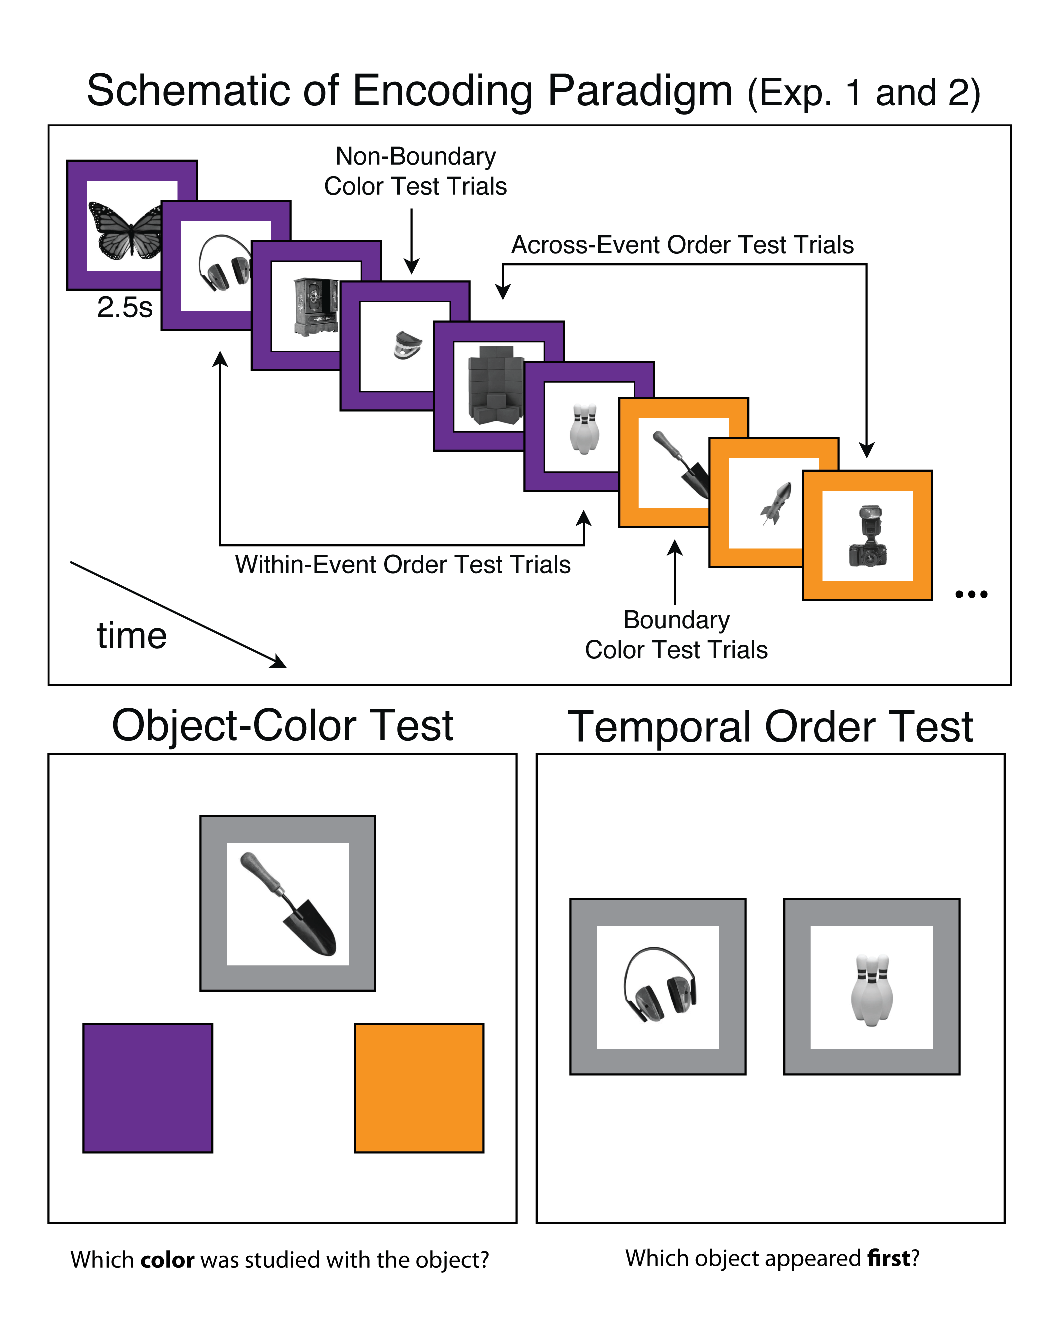
\includegraphics{figures/chapter1_figure1}
\caption{This is the caption}
\end{figure}

The goal of Experiment 1 was to assess whether perceptual event
boundaries increased object-color associative memory. We predicted that
the memory enhancement would be specific to the boundary object-color
pair. A pattern of this nature would suggest a transient memory effect,
perhaps driven by a boundary-driven allocation of attentional resources
\autocite{kurby_segmentation_2008}.

\subsection{Methods}\label{methods}

\subsubsection{Participants}\label{participants}

Participants were 26 individuals (ages 18-35) recruited from New York
University and the greater New York Metropolitan Area. All participants
gave informed written consent in accordance with the University
Committee on Activities Involving Human Subjects (UCAIHS) and
participated in exchange for monetary compensation. We excluded
participants with chance memory performance (N = 2), leaving 24
participants for the statistical analyses. For all three experiments,
the sample size was chosen based on a power analysis (power = .8, alpha
= .05) of a separate study on boundary-related memory effects from
\textcite{dubrow_influence_2013}.

\subsubsection{Materials}\label{materials}

For all experiments, we used a stimulus set consisting of 576 gray-scale
pictures of objects from various online databases. A subset of these
stimuli was used for Experiment 1 (432 objects). Each one was resized to
a fixed size of 350x350 pixels. To generate colors for the frames, 24
unique colors were selected from color continuum ranging from
{[}0,0,0{]} to {[}255, 255, 255{]} RGB values. Lists of colors for each
block were generated, such that no two colors that occurred
consecutively at encoding could be perceptually similar. For example, if
the previous event color was red, the next color could not be orange,
but it could be blue or green. Furthermore, the same color could not
appear in a list more than once and colors were recycled after every
four lists. Stimulus order varied for each subject and stimulus-color
pairings were randomized across subject.

\subsubsection{Design and Procedure}\label{design-and-procedure}

Before the experiment began, there was a brief practice version of the
experiment to ensure that participants understood the task. For each of
12 study lists, participants intentionally encoded lists of 36
trial-unique gray-scale objects that were embedded on a colored frame.
Participants were instructed to imagine the object in the color of the
frame and decide if the object-color pair was pleasing. The participants
were instructed to respond as soon as they made a pleasantness decision
by pressing one of two buttons on the keyboard (`j' or `k'). The color
of the frame was identical for six consecutive objects before switching
to a new color for the next six objects. An `event' was defined as six
consecutive objects with the same colored frame. There were six events
per study list. On `boundary' trials, the frame color updated at trial
onset (i.e.~concurrently with the object). All other trials (event
positions 2-6) were called `non-boundary' trials. Objects were presented
for a fixed time of 2.5 seconds (s) with a fixed 2 s inter-trial
interval (ITI) followed by a .5 s fixation cross before the onset of the
next trial. The colored frame remained on the screen continuously during
the presentation of each event (including the 2 s ITI and a .5 s
fixation cross) and only changed concurrently with boundary objects. It
is important to note that the objects remained on the screen for a fixed
period of time (2.5 seconds). Thus, encoding response times in the rest
of this manuscript refer to the amount of time it took for the
participant to complete the pleasantness decision, not the duration that
the stimulus was on the screen.

Following each encoding list, we tested object-color associative memory.
To minimize recency memory effects, the test was structured such that
objects presented in the first half of the experiment (1:18) were tested
first and objects presented in the second half of the experiment (19:36)
were tested second. However, within each half, the test trials were
randomized. For each test trial, participants were shown a previously
studied object with a grey border presented above two colors that were
positioned on the left and right side of the computer screen (Figure 1).
One of these colors (target) was originally paired with the object while
the other color (lure) was always one of the colored frames that had
immediately preceded or followed the target color at encoding. The lure
was counterbalanced such that it was equally likely to precede or follow
the target color. Targets and lures were also equally likely to appear
in the left or right positions on screen. In one step, participants were
asked to indicate which of the two colors had been paired with the
object at encoding and also to indicate their confidence in their
decision (high/low confidence, HC/LC). Thus, there were a total of 4
possible responses during the test (HC left color, LC left color, HC,
right color, LC right color). Test trials were self-paced and advanced
as soon as a response was given, with a fixed .5 s ITI between test
trials. Half of the items in each encoding list were tested: We
alternated between testing of even (2:2:36) and odd (1:2:36) trials on
each list.

\subsection{Results}\label{results}

\begin{figure}[htbp]
\centering
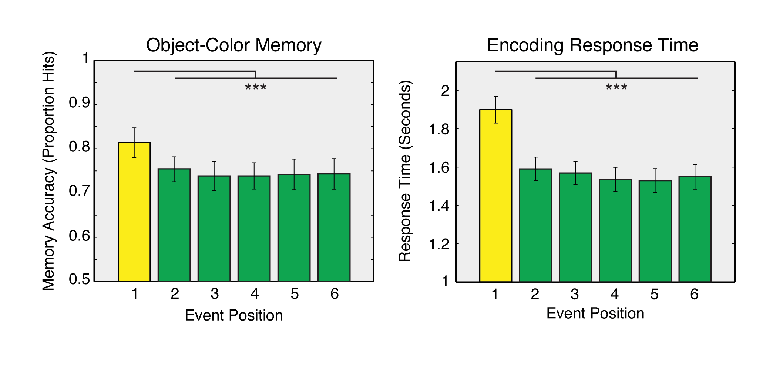
\includegraphics{figures/chapter1_figure2}
\caption{This is the caption}
\end{figure}

\subsubsection{Effect of perceptual boundaries on color memory
performance.}\label{effect-of-perceptual-boundaries-on-color-memory-performance.}

We found that memory for the object-color association varied as a
function of event position {[}Figure 2; \emph{F}(5,115) = 5.23, \emph{p}
\textless{} .001, \(\eta^{2}\) = .185{]}. The position by confidence
interaction was not significant {[}\emph{F}(5,109) = .42, \emph{p}
\textgreater{} .1{]}, so we collapsed across high and low confidence
trials. A planned contrast revealed that color memory was significantly
better for the boundary condition compared to non-boundary conditions
{[}\emph{t}(23) = 5.54, \emph{p} \textless{} .001, Cohen's \emph{d} =
1.66{]} and follow up pairwise t-tests show that memory for the boundary
condition was significantly better than each non-boundary condition
{[}\emph{p}'s \textless{} .05{]}. Thus, object-color associative memory
at boundaries was significantly enhanced relative to trials that are not
studied at perceptual boundaries.

\subsubsection{Encoding Response times}\label{encoding-response-times}

Next, we asked whether perceptual boundaries also impacted RTs during
the successful retrieval of the object-color associations. We found that
RTs to correctly remembered trials varied as a function of event
position {[}\emph{F}(5,115) = 4.112, \emph{p} \textless{} .002,
\(\eta^{2}\) = .152{]}. The position by confidence interaction was not
significant, so we collapsed across confidence {[}\emph{F}(5,95) = 1.23,
\emph{p} \textgreater{} .1{]}. A planned contrast revealed that
retrieval of items from the boundary condition was significantly faster
than the non-boundary conditions {[}\emph{t}(23) = -3.01, \emph{p}=.006,
Cohen's \emph{d} = .88{]}. Subsequent pairwise t-tests revealed that
position 1 was significantly faster than positions 2, 4 and 6
{[}\emph{p}'s \textless{} .05{]}, and a trend for an effect for position
3 {[}\emph{p} = .059{]} and 5 {[}\emph{p} = .068{]}. Thus, during
retrieval, RTs to correct boundary trials were speeded relative to
non-boundary trials, suggesting that information studied at boundaries
is more accessible than non-boundary information.

\subsection{Discussion}\label{discussion}

Experiment 1 revealed that associative memory was enhanced for trials
that appeared at perceptual event boundaries. Prior studies that have
reported better overall memory for information studied at event
boundaries
\autocites{boltz_temporal_1992}{newtson_perceptual_1976}{schwan_cognitive_2004},
used clips from studied movies as retrieval cues and these cues taken
from event boundaries contained more diagnostic information about the
clips, which could ultimately account for the memory benefit. By
contrast, in the present study, the only difference between the boundary
and non-boundary conditions was a change in the color of the background
frame in the boundary condition. Therefore, during retrieval, the amount
of available perceptual information on each test trial was the same and
so, any differential effects we see in boundary memory must be related
to processes that occurred during encoding. Thus, the current finding is
consistent with these prior results but importantly extend them to a
situation where the retrieval content is matched, which implicates that
processes that occur at the time of the boundary itself are responsible
for enhancing memory for boundary information.

In one relevant study, \textcite{swallow_event_2009} found that memory
for objects occurring at event boundaries was better than memory for
non-boundary objects when object recognition memory was probed very
shortly after (\textasciitilde{}5 seconds) an event boundary, but not
when memory was probed within the same event. The authors interpreted
this effect to suggest that retrieving across event boundaries relies on
the access of long-term item representations (as opposed to accessing
working memory representations). They reasoned that since EST predicts
better encoding of boundary information into long-term memory, the
recognition memory difference for boundary and non-boundary objects
should be maximal when the test occurs after an event boundary. The
results of the current experiment are consistent with the results of
this prior study. However, our study is novel in a few critical ways:
First, we test memory after a substantially longer delay
(\textasciitilde{}3-5 minutes as compared to \textasciitilde{}5
seconds). This confirms the claim that long-term boundary memory is
enhanced, rather than a difference in working memory accessibility
between boundary and non-boundary information. Second, we test
associative memory between an object and its accompanying color
background rather than item memory. Thus, our findings extend previous
work to suggest that at event boundaries, items are more strongly bound
to their context (i.e.~the color background). Finally, while the
previous study used naturalistic movies as their stimuli, we opted for a
simpler stimulus set consisting of objects and color backgrounds. While
there are undoubtedly benefits to using naturalistic stimuli, our choice
of simple object and color associations allowed us to carefully control
for the quantity and quality of information available at event
boundaries. Thus, the current experiment supports and extends previous
work on boundary-related memory enhancements.

Another related study showed that switching encoding tasks midway
through a short list of words resulted in a significant increase in the
free recall of words that followed the task switch (specifically, n and
n+1) relative to recall of items (in the same serial position) of a
control list with only one task \autocite{polyn_task_2009}. Although
interpreted as evidence for the notion that task context serves as a
retrieval cue, the task switch may have additionally acted as an event
boundary thus, facilitating the encoding of words that followed it.
While the effect reported in \textcite{polyn_task_2009} compared lists
containing a task switch to lists with no task switch, the
boundary-related memory enhancement reported here is relative to other
non-boundary items within the same list (as opposed to lists with no
boundaries). Another notable difference between the studies is that
Polyn utilized a free recall task to probe memory, whereas, in the
current study, we used a forced-choice associative recognition test. If
free recall of the boundary item `reinstates' its associated temporal
\autocites{howard_distributed_2002}{polyn_context_2009} or source
\autocites{frost_clustering_1971}{hintzman_memory_1972}{murdock_modality_1969}{nilsson_further_1974}{polyn_task_2009}
context, the context reinstatement could act as a cue to facilitate
retrieval of neighboring items, and result in enhanced memory for items
that neighbored the boundary item. Thus, the enhancement of items
following the boundary item in the free recall study could be driven by
organizational processes during retrieval, rather than boundary-driven
segmentation during encoding. In contrast, retrieval processes are
unlikely to interact with the boundary enhancements reported in the
current study because we probed associative recognition memory and the
amount of retrieval content was matched between conditions. However,
importantly, both studies employ a shift in processing during study to
evoke a boundary and see that information encountered at a boundary are
more likely to be remembered.

This enhancement in memory observed at event boundaries is also
reminiscent of the Von Restorff effect, the empirical finding that items
with features that are novel within the local context of an experiment
are better remembered
\autocites{restorff_uber_1933}{ranganath_neural_2003}. However, this
study is unique in that we don't test item memory, but rather we measure
associative memory between the encoded item and the contextual feature
that changed (a colored background in this case). Furthermore, it
emphasizes the transient nature of novelty-driven associative memory
encoding: we observed an associative memory enhancement specifically
that the boundaries where associative memory for the remaining
non-boundary positions are reduced and not significantly different from
one another. One explanation for the boundary-related memory
enhancements we observed here is that the switch in context drives
attention toward the novel feature in the environment (the colored
background) and since attentional priority is high for this trial,
binding between the object and the color is boosted. Thus, the memory
benefit could be a result of novelty driven attentional priority. In
summary, these results add to a growing body of literature suggesting
that contextual novelty, or event boundaries, promote memory encoding.

One final, but important, point is that in this experiment and the two
that follow, the color background was a task-relevant feature of the
experiment. Participants made pleasantness judgments on the object color
pairing. When the context is task relevant, we see a boost in
item-context binding at event boundaries. Whether or not task relevance
of the context is a necessary part of the experimental design should be
addressed in future research.

\section{Experiment 2: Perceptual boundaries facilitate object-color
binding, but reduce across-event temporal order
memory.}\label{experiment-2-perceptual-boundaries-facilitate-object-color-binding-but-reduce-across-event-temporal-order-memory.}

\subsection{Introduction}\label{introduction-1}

Experiment 1 provided evidence that associative binding is enhanced for
local representations encountered at event boundaries compared to those
encountered in the midst of an event (i.e.~non-boundary items). The
enhancement in binding representations present at event boundaries is
consistent with the notion that attention to boundary representations is
enhanced. If this is the case, then we reasoned that another form of
memory, namely temporal order memory, may be disrupted. If perceptual
boundaries caused a shift in attention to the novel color information,
then the associative binding between pairs of items flanking that
boundary would be disrupted. Indeed, prior experiments using temporal
shifts in narrative as well as category and task switches at boundaries
has shown this to be the case
\autocites{dubrow_influence_2013}{ezzyat_what_2011}{ezzyat_similarity_2014}.
Thus, we aimed to extend that work and see if boundaries as defined in
this paradigm (i.e.~the color shifts) are associated with reduced
temporal order memory. Thus, in Experiment 2, we assessed the effect of
perceptual boundaries on temporal order memory, as well as object-color
associative memory. Furthermore, this experimental design allowed us to
ask whether temporal order memory for pairs items encountered across an
event boundary is related to the enhanced processing of the boundary
information itself. We modified the design of Experiment 1 to include a
temporal order memory test (while keeping the test of object-color
background memory). The encoding task and parameters in Experiment 2
were identical to encoding during Experiment 1, except that we
encouraged subjects to associate items across time to increase temporal
order memory performance. After each encoding list, we tested temporal
order memory for object pairs studied within the same event (the
`within-event' condition) and compared that to temporal order memory for
objects studied in two adjacent events (the `across-event' condition),
keeping the actual lag between tested items the same. We also tested
object-color memory after each list. We predicted that perceptual
boundaries would 1) increase object-color associative memory for
boundary trials (replicating Experiment 1), and 2) result in reduced
temporal order memory for objects studied in adjacent events.
Furthermore, we hypothesized that the magnitude of the boundary effect
(i.e.~the time spent processing the boundary item) should be directly
related to the decrement in across-event temporal order memory.

\subsection{Methods}\label{methods-1}

\subsubsection{Participants}\label{participants-1}

Participants were 33 individuals (ages 18-35) recruited from New York
University and the greater New York Metropolitan Area. All participants
gave informed written consent in accordance with the University
Committee on Activities Involving Human Subjects (UCAIHS) and
participated in exchange for monetary compensation. We excluded
participants if their memory performance was not significantly above
chance using a binomial test---this led to exclusion of eight
participants for chance performance on the color and/or order memory
tests. It should be noted that the removal of these subjects did not
influence the statistical outcomes of any of the results reported here.
We excluded these subjects on the premise that it is not sensible to
interpret statistical differences in memory between conditions, when
memory performance is not above chance in the first place. Thus, we
decided to take a conservative approach and removed participants whose
memory performance was not statistical above chance on average. One
additional participant was excluded for failure to press any buttons
during encoding. The remaining 24 participants were used for all
analyses.

\subsubsection{Materials}\label{materials-1}

Materials were the same as Experiment 1. The entire stimulus set was
used for Experiment 2 (576 objects).

\subsubsection{Design and Procedure}\label{design-and-procedure-1}

The design of the encoding was very similar to Experiment 1, except that
we had 16 study/test blocks (compared to 12 in Experiment 1). Following
each encoding list, we tested object-color memory followed by temporal
order memory. To assess object-color memory, we tested two items from
each event. Objects that appeared concurrently with a change in the
color frame made up the ``boundary'' color condition (B). Objects that
were studied in the middle of the list (specifically, in the 4th
position of the event) made up the ``non-boundary'' color condition
(NB). To assess temporal order memory, participants made order judgments
on pairs of items: objects studied in the second and sixth positions of
each event were paired together and made up the ``within-event'' (WE)
order condition. Objects that were studied in the fifth and third
positions of two adjacent events were paired together and made up the
``across-event'' (AE) order condition. Note that a given item was never
tested more than once. An item was either tested for color memory or
temporal order memory (but never both). There were a total of 80 test
trials for each of the four conditions.

The only procedural difference during encoding (compared to Experiment
1) was that participants were encouraged to adopt an associative memory
strategy to promote later temporal order memory. Specifically, we told
participants to imagine the objects interacting with each other over
time. Critically, participants were instructed to associate objects
irrespective of the presence of different color frames. We added this
additional instruction since we reasoned that after the first temporal
order memory test, participants may adopt this kind of strategy to be
successful on temporal order memory judgments in subsequent lists. There
was a short practice session to assure that subjects understood the task
instructions.

After each study list, color memory was tested first, with the same
design as Experiment 1. Following completion of the color memory test,
participants were tested on their memory for the temporal order of pairs
of objects. For each test trial, two previously studied objects appeared
side by side on the screen (Figure 1). Participants were asked to
indicate which of the two objects appeared earlier in the list. The
tested pairs of objects were chosen such that there had always been
three intervening objects between them at encoding. Critically, this was
the case for both within-event and across-event trial-pairs. Thus, the
actual number of intervening items between the two conditions was
constant (3 intervening items) but the across-event test-pairs were
studied with a boundary between them while within-event pairs were
studied with the same color frame (i.e.~in the same event; Figure 1).
Participants were again asked to indicate their confidence in their
decision (high/low). Test trials were self-paced and advanced as soon a
response was given, with a fixed .5 s ITI included between test trials.

\subsection{Results}\label{results-1}

\begin{figure}[htbp]
\centering
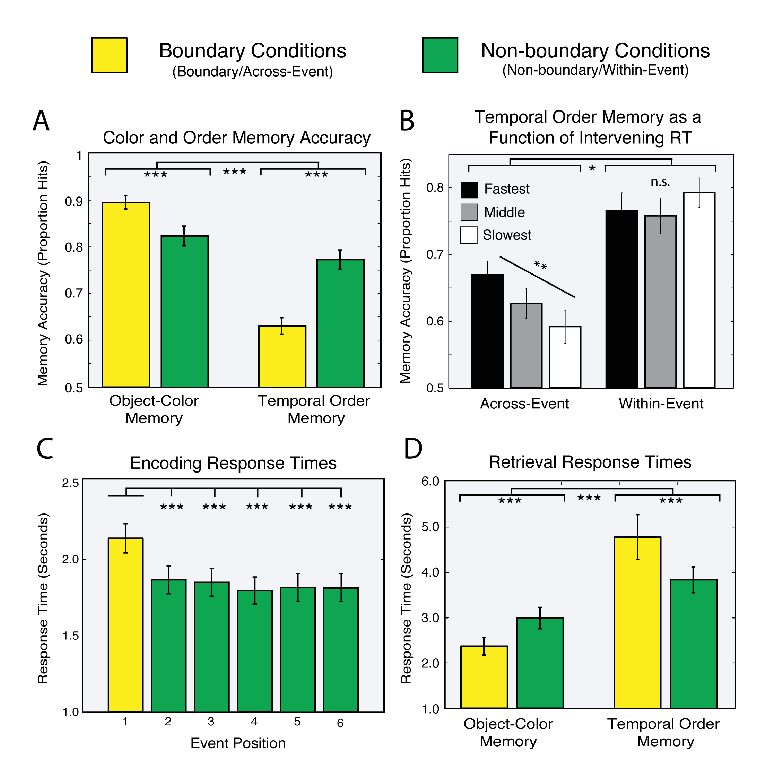
\includegraphics{figures/chapter1_figure3}
\caption{This is the caption}
\end{figure}

\subsubsection{Effect of perceptual boundaries on object-color and
temporal order
memory}\label{effect-of-perceptual-boundaries-on-object-color-and-temporal-order-memory}

Accuracy for object-color memory and temporal order memory was
calculated in two ways: First, we looked at the overall proportion of
correct responses as a function of test condition. Secondly, if the data
varied by confidence, then we separated correct trials by confidence
(HC/LC) and calculated memory accuracy for each condition. Finally, we
assessed whether there was an interaction between boundary/non-boundary
status and memory test type (color/order).

We found that object-color memory accuracy for boundary trials was
significantly better than non-boundary trials {[}\emph{t}(23) = 5.80,
\emph{p} \textless{} .001, Cohen's \emph{d} = 1.96; see Figure 3a{]}.
There was no condition by confidence interaction, so we did not separate
the data by confidence {[}\emph{F}(1,23)=.73,
\emph{p}\textgreater{}.1{]}. These analyses suggest that the event
boundary significantly increased memory for the object-color
association. This result replicates the boundary-related memory
enhancement reported in Experiment 1.

By contrast, temporal order memory was significantly better for the
within-event condition relative to the across-event condition
{[}\emph{t}(23) = 5.37, \emph{p} \textless{} .001, Cohen's \emph{d} =
1.53{]}. There was a significant condition by confidence interaction
{[}\emph{F}(1,23) = 11.01, \emph{p}\textless{}.003, \(\eta^{2}\) =
.33{]}, such that the effect was stronger for HC responses
{[}\emph{t}(23) = 6.008, \emph{p} \textless{} .001, Cohen's \emph{d} =
1.78{]} than LC responses {[}\emph{t}(23) = 2.07, \emph{p} = .05,
Cohen's \emph{d} = .63{]}. Taken together with the data above, this
suggests that the boundaries led to a reduction in associative memory
across events while simultaneously increasing associative binding of
representations at the boundary itself. To directly test for this
interaction, we performed a two-way repeated measures ANOVA and found a
significant test type (color/order) by condition (Boundary/Across-event
and Non-boundary/Within-event) interaction {[}Figure 3a; \emph{F}(1,23)
= 45.39, \emph{p} \textless{} .001, \(\eta^{2}\) = .66{]}. This data
shows that perceptual boundaries improved object-color memory at the
boundary itself, but disrupted temporal order memory for object pairs
that spanned the boundary. Together, these findings suggest a
boundary-related trade-off, where memory for boundary information is
enhanced, perhaps at the cost of across-event associative binding.

\subsubsection{Across-event temporal order memory negatively related to
boundary
processing}\label{across-event-temporal-order-memory-negatively-related-to-boundary-processing}

As a further means for asking whether there is a trade-off between
boundary processing and these different forms of memory, our next
analysis assessed whether response times to boundaries at encoding were
related to later color and order memory. We reasoned that increased
encoding response times to boundary items might reflect greater
attention to the item and color on boundary trials and may, in turn, be
related to the temporal order reductions. Thus, we hypothesized that
longer boundary response times may result in worse order memory for
pairs of objects that spanned the boundary. Crucially, however, we
expected no such relationship between non-boundary response times and
temporal order memory for within-event trial pairs.

To test this hypothesis, we first performed a logistic regression using
boundary response times (i.e.~task responses to position 1 items) to
predict across-boundary temporal order accuracy (position 5 and 3
items). We found that there was an inverse relationship, such that
longer boundary response times were related worse temporal order memory
{[}mean slope = -.18, \emph{t}(23) = -2.16, \emph{p} \textless{} .05,
Cohen's \emph{d} = .44{]}. Critically this effect was not present when
we used non-boundary response times (i.e.~task response times to
position 4 items) to predict within-event temporal order memory
(position 2 and 6 items) {[}mean slope = .19, \emph{t}(23) = 1.32,
\emph{p} \textgreater{} .1{]}. Furthermore, a paired t-test revealed
that the regression slope for the boundary condition was significantly
more negative than the non-boundary regression slope {[}\emph{t}(23) =
-2.35, \emph{p} \textless{}. 05, Cohen's \emph{d} = .66{]}, suggesting a
specific relationship where longer boundary response times were related
to worse across-event temporal order memory.

As a second approach to test this hypothesis, we divided boundary
encoding response times into terciles and assessed temporal order memory
separately for each bin. This complementary analysis allowed us a way to
better visualize the data as well as a way to reduce some of the
variance of response times driven by noise. To test whether boundary
(but not non-boundary) response times are related to temporal order
memory, we conducted a two-way repeated measures ANOVA. There was a
significant condition (boundary/non-boundary) by response time tercile
(slowest, middle, fastest) interaction {[}\emph{F}(2,46) = 4.23,
\emph{p} \textless{} .05, \(\eta^{2}\) = .156{]}. This interaction was
driven by the fact that order memory performance was the lowest in the
slowest tercile of response times and was the best in the fastest
tercile of boundary response times {[}Figure 3b; fastest vs.~slowest:
\emph{t}(23) = 3.03; \emph{p} = .005, Cohen's \emph{d} = .88{]}.
Crucially, no effect of response time on order memory for the analogous
intervening trial in the non-boundary condition was evident {[}fastest
vs.~slowest: \emph{t}(23) = -1.20; \emph{p} =.24{]}. That is, the
response time to the item in the 4th event position was not related to
within-event order memory (between the items in the 2nd and 6th event
position). Furthermore, there was a significant linear trend for
across-boundary temporal order memory as a function of boundary response
tercile {[}\emph{F}(1,23) = 9.23, \emph{p} = .006, \(\eta^{2}\) =
.286{]} that was not present for the analogous within-event condition
{[}\emph{F}(1,23) = 1.44, \emph{p} \textgreater{}.1{]}, and there was a
significant condition (boundary vs.~non-boundary) by tercile (slowest,
middle fastest) interaction in the linear term {[}\emph{F}(2,46) = 4.23,
\emph{p} \textless{} .05, \(\eta^{2}\) = .25{]}, suggesting that the
linear trend was specific to the across-boundary condition. These data
support the notion that event boundaries disrupt temporal order memory
and provide evidence that response time variability on boundary trials
is related to the outcome of temporal order memory for the trials that
span the boundary. In contrast, response times to an intervening item
within events do not appear to be related to temporal order memory.

We then ran a separate control analysis to test whether this
relationship between boundary response time and temporal order memory
was specific to the boundary item. It's possible that rather than
temporal order memory being specifically related to processing at the
boundary, memory could vary as a function of the overall speed of
processing across the sequence of items. In other words, order memory
could vary as a function of the mean encoding response time across the
tested items (i.e.~all trials that intervened the later tested items),
rather than to the boundary item specifically. To address this, we
averaged encoding response times across sequences of items that crossed
a boundary, where the flanking items of the sequence were boundary
temporal order test pairs. Importantly, we excluded the boundary
response itself, but included the other intervening items. Then, we
again sorted the data into terciles, and computed temporal order memory
separately for each response time bin. If the relationship between the
speed of boundary response time and temporal order memory were specific
to the processing of the boundary item, then the average response time
across the sequence would not predict temporal order memory. However, if
temporal order memory co-varied with the mean response time across a
sequence, than we would expect a pattern similar to the previous
analysis, where longer response times predicted worse order memory
performance. A one-way ANOVA revealed that mean response time for
sequences of trials that crossed an event boundary was not predictive of
temporal order memory {[}\emph{F}(2,46{]}=.52, \emph{p} \textgreater{}.
1{]}, providing further evidence that boundary processing is
specifically related to across-trial associative encoding. Together with
the accuracy data described above, these results argue for a trade-off
between boundary processing and across-event mnemonic binding.

\subsubsection{Encoding response times}\label{encoding-response-times-1}

Replicating the results from Experiment 1, we see that response times
during encoding varied as a function of within-event position {[}Figure
3c; \emph{F}(5,115) = 50.63, \emph{p} \textless{} .001, \(\eta^{2}\) =
.69{]}, and a planned contrast revealed that task responses on boundary
items (position 1) were significantly slower than non-boundary items
{[}position 2-6; \emph{t}(23) = 8.07, \emph{p} \textless{} .001, Cohen's
\emph{d} = 2.36{]}. Follow up t-tests show that each pairwise difference
is significant {[}1 vs.~2-6, \emph{p}'s \textless{} .001{]}.

\subsubsection{Retrieval response times}\label{retrieval-response-times}

Finally, we compared response times for correct color and order memory
retrieval as a function of condition. The goal of this analysis was to
see whether the relative increase in memory performance we observed in
the previous color and order accuracy analyses (i.e.~Figure 3a) was also
accompanied by a speeding of the retrieval response. To test whether the
pattern of response times across conditions was dependent on confidence,
we conducted a repeated measures two-way ANOVA and assessed the
condition by confidence interaction. The interaction was not significant
for order {[}\emph{F}(1,23) = .15, p\textgreater{}.1{]} or color
{[}\emph{F}(1,23) = .28, \emph{p} \textgreater{} .1{]}, so we collapsed
across confidence. We found that response times for correct color memory
retrieval trials were significantly faster for B trials relative to NB
trials {[}\emph{t}(23) = 7.3, \emph{p} \textless{} .001, Cohen's
\emph{d} = 2.45; Figure 3d{]}. On the order memory test, better
performance on the within-event trials was accompanied by faster
response times relative to the across-event trials {[}\emph{t}(23) =
3.91, \emph{p} \textless{} .001, Cohen's \emph{d} = 2.28{]}.
Additionally, a two-way repeated measures ANOVA revealed a significant
memory test by condition interaction {[}\emph{F}(1,23) = 32.77, \emph{p}
\textless{} .001, \(\eta^{2}\) = .588{]}. In sum, mnemonic
representations in conditions with better memory (boundary object color
and within-event temporal order) were also accessed more quickly at
retrieval.

\subsection{Discussion}\label{discussion-1}

The results of the Experiment 2 provide evidence that while associative
memory was enhanced for representations presented at perceptual
boundaries, these boundaries resulted in a decrease in temporal order
memory for items studied in adjacent events (Figure 3a). The reduction
in temporal order memory observed is consistent with previous work
showing event boundary-related reductions in cued recall for narrative
stimuli \autocite{ezzyat_what_2011}, as well as an influence of
boundaries on temporal memory for visual images
\autocites{dubrow_influence_2013}{ezzyat_similarity_2014}.
Interestingly, our temporal order memory effects emerged using a simple
color manipulation, demonstrating that boundary-related temporal memory
disruptions can result from simple changes in a perceptual feature of an
event. Moreover, we found that slower boundary encoding response times
were associated with worse temporal order memory for objects spanning
those boundaries. In other words, the larger the magnitude of the
`boundary effect' (as indexed by response time), the worse the temporal
order memory for pairs of objects that spanned the boundary. The current
data supports previous work by replicating the boundary-related
reduction of across-event temporal order memory and importantly extends
it to suggest a trade-off between boundary processing itself and
across-event order memory. In other words, this data highlights the idea
that orienting to something salient in the environment comes at the cost
of the ongoing maintenance of items over time.

Our finding of relatively better temporal order memory for within-event
items as compared to across-event items is also consistent with buffer
models of episodic memory
\autocites{atkinson_human_1968}{lehman_global_2009}{lehman_buffer_2013}{raaijmakers_search_1981}.
\textcite{lehman_buffer_2013} 's buffer model hypothesizes that during
encoding, a buffer process exists that can maintain or drop information
depending upon the goals of the subject or the demands of the task.
Items and contexts that are maintained in the buffer become
associatively linked, while information experienced in different buffers
does not become as strongly associated. In our task, we hypothesize that
items encountered in the same color are maintained in the same buffer
whereas a switch in color (i.e.~perceptual event boundary) may serve as
a cue for the brain to flush the contents of the current buffer, thus
creating an associative disconnect between items studied in different
contexts. Thus, one possible explanation for our observed difference
between within and across event temporal order memory is that items
encountered within the same event occupy the same buffer and thus are
more strongly bound to each other than items encountered in different
events (i.e.~distinct buffers).

Buffer models of episodic memory have been quite successful at
accounting for patterns in episodic memory, particularly in studies with
an intentional forgetting component \autocite{lehman_buffer_2013}.
Typically in these studies, at the end of an encoding list, subjects are
instructed on whether or not to forget the previously studied list. The
model predicts that the cue to forget causes a flushing of the
previously studied items from the buffer (a buffer operation the authors
call ``compartmentalization''). One major difference between our study
and these prior studies is that we do not explicitly instruct
participants to forget between events. In fact, we encourage
participants to bind together items irrespective of the background
color. Thus, a possible interpretation of our findings is that
perceptual event boundaries serve as a bottom-up cue that triggers the
brain to remove the contents of the current buffer. Thus,
compartmentalization may occur spontaneously if there is sufficient
perceptual change in the environment. Future work should be conducted to
characterize whether the nature of the task (i.e.~top-down vs.~bottom-up
compartmentalization) has differential consequences for the organization
of events in episodic memory.

Finally, the memory `trade-offs' reported here can be contrasted with a
body of literature investigating block-level or instruction-level
trade-offs in item vs.~associative in formation in memory
\autocites{einstein_levels_1980}{gronlund_time_1989}{hockley_tests_1996}{hunt_relational_1981}{sharps_relational_1992}.
In this literature, the overarching theme is that when item encoding is
prioritized over associative or relational encoding, item memory
benefits and associative memory suffers. In contrast, when associative
memory is prioritized, there is a benefit for associative memory but
interestingly, item memory remains intact. In the current work, we show
that at event boundaries, when attention is presumably redirected from
item-item associative processing to more local item-context processing,
across-event temporal order memory suffers, while boundary item-context
memory is enhanced. To coalesce these findings, it appears that
regardless of whether the manipulation is top-down and extended in time
(such as an instructional manipulation) or bottom-up and dynamic (such
as a perceptual event boundary in the current design), attention to
`in-the-moment' representations trades off with more temporally extended
relational encoding (i.e.~focusing on item-item relationships). Thus, in
contrast to previous work, the results reported in the current study
highlight the temporally dynamic nature of item and relational tradeoffs
during episodic memory encoding.

\section{Experiment 3: Perceptual boundaries impose structure on verbal
free
recall}\label{experiment-3-perceptual-boundaries-impose-structure-on-verbal-free-recall}

\subsection{Introduction}\label{introduction-2}

So far, we've provided evidence that perceptual boundaries enhance
boundary-related associative memory, while simultaneously reducing
across-event temporal order memory, and that the magnitude of the
boundary effect is predictive of the cost in temporal order memory. One
intuitive explanation for this pattern of results is that when
encountering a perceptual boundary, there is a shift in attention to the
processing of the novel color information, which trades off with the
integration of the previous item representation (i.e.~the pre-boundary
trial) and the current (boundary) trial. We reasoned that if
within-event item representations are more strongly integrated than
items that span a boundary, then one might expect within-event items may
be represented more similarly in memory. If asked to recall the items,
this could lead to a greater likelihood of sequentially recalling
within-event items relative to across event items. Thus, in Experiment
3, we tested the hypothesis that the likelihood of making a local
forward transition (e.g.~n+1, n+2, n+3) from boundary items to other
within-event items would be greater than the likelihood of a local
forward transition from pre-boundary items, where forward transitions
would be to items in a new event.

To test this hypothesis, we employed a modified version of the encoding
paradigm used in Experiments 1 and 2 that was optimized to test memory
using verbal free recall (see Design for details). In this experiment,
participants encoded lists of visual objects embedded in a colored frame
with an accompanying verbal label, and after a short distractor task
were instructed to verbally recall as many items as possible.
Critically, like the previous experiments, the studied objects were
embedded on a colored frame that periodically changed in color.

\subsection{Methods}\label{methods-2}

\subsubsection{Participants}\label{participants-2}

Participants were 24 individuals (ages 18-35) recruited from New York
University and the greater New York Metropolitan Area. All participants
gave informed written consent in accordance with the University
Committee on Activities Involving Human Subjects (ACAIHS) and
participated in exchange for monetary compensation. One person was
excluded for chance color memory performance, leaving 23 participants
for all analyses.

\subsubsection{Materials}\label{materials-2}

For this experiment, we used a subset of the objects (totaling 384
grey-scale objects) used in Experiments 1 and 2. We also included a
written label displayed below each presented object to encourage
participants to use the same label during verbal recall. Each list was
designed to have minimal conceptual overlap, to minimize confusion
during free recall scoring as well as semantic clustering at retrieval.

\subsubsection{Design}\label{design}

In this experiment, participants studied lists of 24 objects (along with
a written label) embedded in a colored frame that changed to a new color
after every 4 trials. Like the previous experiments, there were 6
`events' and 5 `event boundaries' per list. We chose to present 24 items
per list rather than 36 (as in Experiment 1 and 2) due to pilot data
suggesting poor free recall performance when longer study lists were
used. Additionally, we reduced event length from 6 to 4 items to ensure
adequate power for the free recall analyses (i.e.~to have sufficient
boundary trials). Like Experiments 1 and 2, trials that were studied
concurrently with a color change are considered ``boundary'' trials and
objects studied in the other event positions (2-4) are called
``non-boundary'' trials.

\subsubsection{Procedures}\label{procedures}

For each list (12 total), participants encoded 24 object-color pairs.
Participants were instructed to imagine the object in the color of the
frame and make a pleasantness judgment on the object/color combination.
After each study list, participants completed a distractor task in which
they were asked to indicate whether arithmetic problems were correct or
incorrect (e.g. ``5+4+2=11?''). The numbers 1-6 were used for the
arithmetic problems, and the probability of the answer being correct was
50\%. Each problem was presented for 3 seconds for a total of 10
problems during each distractor period (30 seconds). They were also
given immediate feedback to encourage engagement. Following the
distractor task, participants were presented with a screen prompting
them to say ``Next Block'' and then verbally recall as many words as
they could. They were given a minimum of 90 seconds and told to use more
time if they felt they could recall more words. A schematic of a block
of the experiment is displayed in Figure 4a.

Audio was recorded throughout the entire session. Unclear responses were
excluded from the analysis. Synonyms to words that were actually studied
were not considered correct responses. For example, if the correct
response was ``panther'' and the subject reported ``leopard'', this
would not be considered a correct response. However, partial answers
were counted as correct. For example, if the correct response was ``toy
train'' and the subject responded ``train'', it would be marked as
correct. The total number of excluded trials (combining across synonyms,
unclear responses and prior list intrusions) was small (3.7\%). Analysis
of the free recall audio files was performed by one author and one
research assistant using Penn TotalRecall,
(http://memory.psych.upenn.edu/TotalRecall). Using this program, the
onset and serial recall order of each retrieved object was recorded.
Crucially, scorers were blind to the encoding condition to which each
object belonged.

After each free recall period, participants were given an object-color
memory task following the same protocol as Experiments 1 and 2. The
object-color memory test was self-paced. For this experiment, we tested
color memory for all 24 studied items in the list. Across the entire
experiment, there were a total of 36 color memory test trials for each
condition (event positions: 1-4).

\subsection{Results}\label{results-2}

\begin{figure}[htbp]
\centering
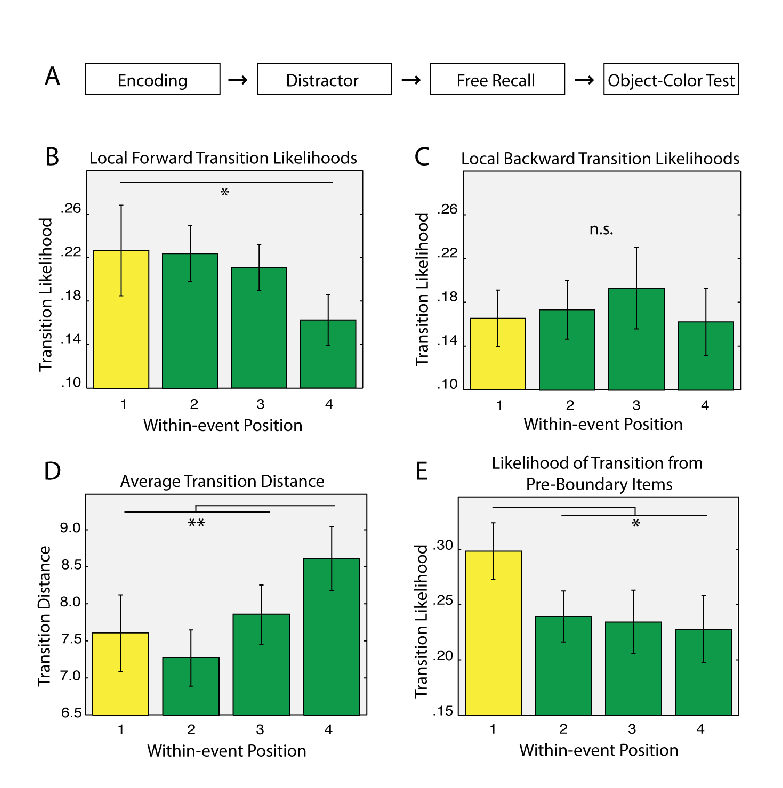
\includegraphics{figures/chapter1_figure4}
\caption{This is the caption}
\end{figure}

\subsubsection{Free recall performance}\label{free-recall-performance}

\emph{Overall performance.} Participants recalled an average of 31.30\%
(\(\sigma\) = 12.6\%) of the items presented for each list (or 7.51 out
of 24 items per list). As expected, free recall varied as a function of
serial position of the list {[}\emph{F}(23,506) = 6.82, \emph{p}
\textless{} .001, \(\eta^{2}\) = .237, Supplemental Fig. 1{]}, where
items at the beginning and the end of the list were more likely to be
recalled than items in the middle of the list
\autocite{murdock_serial_1962}. We also computed free recall performance
as a function of event position within an event, but did not observe an
effect {[}\emph{F}(3,66) = .96, \emph{p} \textgreater{} .1{]}, meaning
that all event positions 1-4 were equally likely to be recalled. We
discuss the implication of this finding in more detail in the general
discussion.

Then, we computed the mean lag-conditional response probability
(lag-CRP) curve (Supplemental Figure 2; see
\autocite{kahana_associative_1996}) which showed that, given free recall
of an item, participants were most likely to make free recall
transitions to items in neighboring list positions, consistent with
previous reports
\autocites{howard_distributed_2002}{kahana_associative_1996}.

\emph{Local transition probabilities in free recall.} To measure the
influence of perceptual event boundaries on free recall, our next
analysis focused on local transition probabilities. That is, given the
recall of item n, what is the likelihood of the next item recalled being
locally forward (i.e.~n+1, n+2, or n+3) or locally backward (i.e.~n-1,
n-2, or n-3)?. First, we focused on local forward transitions up to a
lag of three because for boundary items, local forward transitions would
be to other within-event items whereas for pre-boundary items
(i.e.~position 4 items), local forward transitions would be to items in
the next event. We predicted that there would be a greater likelihood of
local forward transitions from boundary items as compared to
pre-boundary items due to the fact that local forward transitions from
boundary items would be to other within-event items. To test this
prediction, for each within-event position, we computed the likelihood
of a local forward transition (i.e.~the sum of the number of transitions
from n to n+1, n+2, and n+3) divided by the number of transitions to all
other items. This resulted in a measure representing the proportion of
the time participants made a local forward transition relative to all
other transitions to items elsewhere in the list. Critically, there were
no differences in the total number of items recalled for each
within-event position (see Free Recall Performance Section) and thus,
the above analysis is only sensitive to the order of free recall, rather
than the total number of items recalled. The results of this analysis
are plotted in Figure 4b. Consistent with our hypothesis, we found that
local forward transitions from boundary and pre-boundary items were
significantly different from each other {[}\emph{t}(22) = 1.88, \emph{p}
\textless{} .05, one-tailed, Cohen's \emph{d} = .71{]}, where relatively
more local forward transitions were made from boundary items. This data
is consistent with the idea that perceptual event boundaries influence
the structure of free recall behavior.

Next, we tested the idea that local backward transitions from
pre-boundary items might be relatively more likely than local backwards
transitions from boundary items because for pre-boundary items, local
backwards transitions were to other within-event items. We performed the
same analysis as described above, but now for only local backwards
transitions as a function of within-event position (Figure 4c).
Interestingly, we did not observe the predicted effect that local
backward transitions would be relatively more likely for pre-boundary
items as compared to boundary items {[}\emph{t}(22) = .10, \emph{p}
\textgreater{} .9{]}. To summarize, while local forward transitions were
more likely from boundary relative to pre-boundary items, there was no
difference in the likelihood of backward transitions.

\emph{Distal transition probabilities in free recall.} The intriguing
result that there were no differences in backward transition
probabilities led us to the follow question: If participants are not
transitioning from pre-boundary items to other within-event items
(i.e.~local backward transitions), to which items are they are more
likely to transition? We reasoned that if local forward transitions from
pre-boundary items are relatively unlikely (as compared to boundary
items) and there were no differences in local backward transitions, then
transitions from pre-boundary items must be to more distal items in the
list. To quantify this, we computed the average transition distance as a
function of position (Figure 4d). That is, given the recall of item n,
what is the average lag of the next recalled item? For this analysis,
our hypothesis was that transitions from pre-boundary items would be to
more distal items relative to all other within-event positions. Put
another way, when one recalls the last item in an event, we predicted
that they would be relatively more likely to transition to a distal
item. To test this hypothesis, we computed a contrast of the average
transition distance from pre-boundary items relative to the other
within-event positions. The analysis revealed that the average
transition distance from pre-boundary items was significantly more
distal than the average transition distance from other within-event
positions {[}\emph{t}(22) = 2.63, \emph{p} \textless{} .05, Cohen's
\emph{d} = .48{]}. Furthermore, the direct comparison of average
transition distance from pre-boundary and boundary items revealed that
pre-boundary transitions are significantly more distal than boundary
transitions {[}\emph{t}(22) = 2.55, \emph{p} \textless{} .05, Cohen's
\emph{d} = .39{]}. Thus, compared to other within-event positions, free
recall transitions from pre-boundary trials are to relatively more
distal items providing further support for the idea that perceptual
event boundaries influence the structure of free recall behavior.

\emph{Transitions from pre-boundary items.} Our last free recall
analysis was designed to test the idea that transitions from
pre-boundary items would be disproportionately more likely to boundary
items relative to items in other within-event positions. We predicted
that given the recall of the last item in an event (and thus terminating
the recall of a particular episode), one might initiate a memory search
process in an attempt to recall additional items. If boundary items
somehow `stand out' in memory
\autocites{radvansky_across_2012}{zacks_event_2007}, then the likelihood
of transitioning to a boundary item given the recall of a pre-boundary
item may be relatively higher than transitioning to other within-event
positions. In this way, boundary items may serve as a `gateway' into an
episodic event. To test this prediction, we computed the conditional
likelihood of transitioning to each within-event position given the
recall of a pre-boundary item (Figure 4e). A contrast of pre-boundary
transitions to boundary items relative to items in other positions
suggests that following the recall of a pre-boundary item, boundary
items are most likely to be recalled next {[}\emph{t}(22) = 1.89,
\emph{p} \textless{} .05, one-tailed, Cohen's \emph{d} = .79{]}. The
direct comparison of pre-boundary transitions to boundary items
vs.~pre-boundary items showed a significant trend {[}\emph{t}(22) =
1.59, \emph{p} = .063, one-tailed, Cohen's \emph{d} = .52{]}. One
potential issue with the analysis described above is that the effect
could be driven solely by local forward transitions (i.e.~a temporal
contiguity effect). To rule out this explanation, we performed the
analysis again, now removing all local transitions (n +/- 1, 2 or 3).
When analyzing only transitions from pre-boundary items to other distal
items (greater than 3 positions away), the effect remained
{[}\emph{t}(22) = 1.73, \emph{p} \textless{} .05, one-tailed, Cohen's
\emph{d} = .60{]}. Thus, consistent with our prediction, following the
recall of the last item in an event, distal boundary items are
significantly more likely to be recalled next (as compared to other
within event positions). Together with the free recall analyses
described above, these data support the idea that perceptual boundaries
introduce structure into free recall behavior.

\subsubsection{Color memory performance}\label{color-memory-performance}

Analysis of variance revealed a trend for color memory to vary as a
function of within-event position {[}\emph{F}(3,66) = 2.57, \emph{p} =
.06, \(\eta^{2}\) = .11{]}. A planned contrast demonstrated object-color
memory was better for boundary trials than non-boundary trials
{[}\emph{t}(22) = 2.67, \emph{p} = .01, Cohen's \emph{d} = .80{]}.
Post-hoc pairwise t-tests revealed that memory was significantly better
for boundary trials than all non-boundary trials {[}\emph{p}'s
\textless{} .05{]} with no other significant differences. The
interaction between confidence and condition was not significant. Note
that in this experiment we replicate Experiments 1 and 2 show that
boundary object-color memory accuracy was better than non-boundary
memory. While the effect was modest in this version of the paradigm,
together with the color memory enhancements observed in both Experiments
1 and 2, these results provide consistent evidence for boundary-related
memory enhancements.

Response times for correct color memory retrieval trials also varied as
a function of within-event position {[}\emph{F}(3,66) = 10.29, \emph{p}
\textless{} .001, \(\eta^{2}\) = .319{]}. A planned contrast between
boundary and non-boundary color retrieval RTs revealed that boundary RTs
were significantly faster than non-boundary RTs {[}\emph{t}(22) = -4.24,
\emph{p} \textless{} .001, Cohen's \emph{d} = 1.26{]}. Post-hoc tests
showed that color retrieval RTs were significantly faster for boundary
trials compared to all non-boundary trials {[}\emph{p}'s \textless{}
.05{]}. There was no significant interaction between condition and
confidence, so these analyses were performed on data collapsed across
condition.

\subsubsection{Encoding response times}\label{encoding-response-times-2}

There was a significant effect of event position on encoding response
times {[}\emph{F}(3,66) = 28.90, \emph{p} \textless{} .001, \(\eta^{2}\)
= .57{]}. A planned contrast reveals that boundary response times were
significantly slower than non-boundary {[}\emph{t}(22) = 6.72, \emph{p}
\textless{} .001, Cohen's \emph{d} = 2.04{]}. Pairwise t-tests revealed
that boundary encoding response times were significantly slower than all
non-boundary trials {[}event positions 2-4, \emph{p}'s
\textless{}.001{]} and there were no other differences. This finding
replicates Experiments 1 and 2 and extends it to include shorter events
(four as compared with six items in Experiments 1 and 2).

\subsubsection{Math accuracy}\label{math-accuracy}

Accuracy on the math task was high (\(\mu\) = .89, \(\sigma\) = .08) and
all participants performed statistically above chance.

\subsection{Discussion}\label{discussion-2}

In the current experiment, we aimed to examine whether and how free
recall organization was influenced by perceptual event boundaries.
Overall, we found that transition likelihoods varied as a function of
within-event position (Figure 4). First, our results suggest that local
forward transitions were significantly more likely from boundary items
as compared to pre-boundary items whereas there were no differences
between conditions for local backward transitions (Figure 4b, c).
Second, we found that transitions from pre-boundary were on average to
more distal items than transitions from other within-event positions.
Lastly, transitions from pre-boundary items were most likely to be to
boundary items as compared to other within-event positions. These
findings argue that perceptual event boundaries influence the structure
of free recall behavior.

Our finding that local forward transitions (n+1, n+2, n+3) were more
likely from boundary items than from pre-boundary items is consistent
with the idea that items encountered in the same event are more strongly
associated to each other than items in distinct events. For boundary
items, forward local transitions were all to other within event items,
whereas for pre-boundary items local forward transitions were all to
items in the neighboring event. This result is in line with temporal
context models of memory
\autocites{howard_distributed_2002}{manning_oscillatory_2011}{polyn_category-specific_2005}{polyn_context_2009},
that propose that during the study of a list of stimuli, items are bound
to a slowly-changing representation of context. Although the particular
features (e.g.~semantic, source, temporal) that are included in the
context representation vary according to the specific model, all
retrieved context models propose that when an item is recalled from
memory, the context representation is reinstated and used to guide the
retrieval process. Because the context representations of neighboring
items are most similar, this leads to free recall transitions between
neighboring items, and the overall lag-CRP pattern. Our data are in line
with such a retrieval interpretation to the extent that the perceptual
details associated with each item are also reinstated during recall.
Thus, reinstatement of the color associated with an object may make it
more likely that participants will recall other objects encoded with the
same color.

In a previous study, \autocite{polyn_context_2009} found that when
freely recalling a short list of 12 words that included one task switch
at the halfway point in the list, participants tended to cluster their
recall responses by items that shared an encoding task. That is, more
free recall transitions were made between words that were encoded using
the same task as compared to words encoded under two different tasks.
Our results are consistent with that result and extend it to suggest
that the change in a perceptual feature during experience is sufficient
to impose structure in the free recall of events. While Polyn and
colleagues focused their analyses on the effect of task boundaries on
the likelihood of within- vs.~across-event transitions (irrespective of
the list position of the item), we specifically asked whether items that
flanked a perceptual boundary would show a within-event bias. This
analytic approach allowed us to determine precisely how boundaries
modulate the likelihood of within-event recall transitions.

Interestingly, while we found that local forward transitions are
significantly more likely from boundary items relative to pre-boundary
items, we found no difference between the two conditions in local
backwards transitions. If shared context results in stronger associative
binding between items in the same event, one might expect local
backwards transitions to be relatively greater for pre-boundary items
compared to other within-event positions, since local backwards
transitions would be to other within-event items. While we note that the
aforementioned result is a null finding (and therefore not directly
interpretable), we can offer a few speculations as to why we might not
expect to see an effect. Previous studies suggest that free recall is
reliably bias in the forward direction
\autocites{kahana_associative_1996}{howard_distributed_2002} and
backwards transitions are relatively more rare. We see this pattern in
our data as well (Figure 4b, 4c; Supp Figure 2). Thus, it's possible
that perceptual boundaries exert a substantially stronger effect on
forward transition probabilities. An alternative explanation is that our
experimental design was not sensitive enough to detect the effect of
boundaries on backward transitions (e.g., lists too long, events too
short or boundaries not strong enough). Nonetheless, the fact that that
we do observe a greater likelihood of local forward transitions from
boundary items as compared to pre-boundary items is evidence that
perceptual boundaries do indeed shape free recall behavior.

A second notable observation from this experiment was that the average
transition distance from pre-boundary items was significantly further
than from boundary items. On other words, given the successful recall of
a pre-boundary item, participants were more likely to next recall a more
distal item in the list. One possible explanation for this finding is
that perceptual event boundaries result in a weak associative link
between a pre-boundary item and its neighboring boundary item
\autocites{dubrow_influence_2013}{ezzyat_what_2011}. Because of this
weak associative link, after the successful recall of a pre-boundary
item, a memory search process might be initiated and as a consequence,
more distal item may be subsequently recalled. This finding is
consistent with the idea that event boundaries disrupt associative
binding between items and suggest that transitions following the recall
of the last item in an event are on average more distal than transitions
fro other within-event positions.

Another interesting finding from this experiment was that following the
successful recall of a pre-boundary item, the next item recalled is most
likely to be a boundary item. Given that pre-boundary items are
neighbored by boundary items and that participants generally tend to
transition forward in free recall, this may not seem entirely
surprising. However, this effect remains significant after removing
local items from the analysis, suggesting that when one transitions from
a pre-boundary item to a more distal item, it tends to be a boundary
item. An intriguing interpretation of this finding is that event
boundaries may serve as a `gateway' into an episodic event. In other
words, after successfully recalling the end of a previous event and
during a mnemonic search for more items, boundary items might stand out
as entry points into other mnemonic episodes. Consistent with this
interpretation, we found that on average transitions from pre-boundary
items were more distal than from other positions and out of those distal
transitions, transitions to boundary items were most probable. While the
`gateway' idea is certainly attractive, future studies will be necessary
to determine if this is the most likely explanation for this pattern of
results.

Finally, event segmentation theory suggests that items encountered at
event boundaries may be more memorable than items encountered elsewhere
in an event, possibly due to increased attention at boundaries
\autocites{radvansky_across_2012}{zacks_event_2007}. All three
experiments are consistent with this idea by showing that object-color
memory is better at event boundaries than at other within-event
positions. Interestingly, however, in Experiment 3 we did not observe an
overall increase in free recall of boundary items, as one might have
predicted from EST. While we hesitate to over interpret this null
finding, we can offer some speculation to why we observed this effect.
Rather than boundaries generally boosting memory for boundary
information, boundaries may selectively increase associative binding
between a boundary item and its context. A mechanism of this nature
would predict greater object-color associative memory, but not
necessarily better encoding of boundary items alone. Alternatively,
perceptual boundaries may generally enhance encoding, but our study may
not have been sensitive enough to detect it. Future work will be
necessary to disentangle whether event boundaries differentially
influence item memory vs.~item-context associative binding.

\section{General Discussion}\label{general-discussion}

The studies presented here demonstrate that perceptual boundaries
influence the organization of events stored in long-term memory. In
Experiment 1, we found that perceptual boundaries enhanced associative
binding between an object and a color background. In Experiment 2, we
show that while boundary-related associative memory was enhanced,
temporal order memory for pairs of items that span a perceptual boundary
was disrupted relative to order memory for within-event item pairs.
Furthermore, the magnitude of the boundary effect (i.e.~the response
time to the boundary) predicted the cost in temporal order memory
suggesting a trade-off between boundary processing and across-event
temporal order memory. Finally, in Experiment 3, we found that
participants exhibited recall behavior that was structured by perceptual
event boundaries. Taken together, this work provides compelling evidence
that perceptual boundaries have a lasting influence on the structure of
our memories.

These results add to a growing body of literature characterizing the
influence of event segmentation on long-term memory
\autocites{boltz_temporal_1992}{dubrow_influence_2013}{ezzyat_what_2011}{ezzyat_similarity_2014}{newtson_perceptual_1976}{schwan_cognitive_2004}{zacks_event_2006}.
Previous studies using naturalistic stimuli have provided data
consistent with the idea that information experienced at event
boundaries is better encoded in memory
\autocites{boltz_temporal_1992}{newtson_perceptual_1976}{schwan_cognitive_2004}.
However, there is some concern that these effects could be explained by
differences in the amount of diagnostic information between conditions;
that is, if boundary test items provide a better `summary' of a
particular event than non-boundary test items, one might expect higher
boundary memory that is not driven by event segmentation processes, per
se. By contrast, in the current study, we carefully matched the boundary
and non-boundary conditions during retrieval, such that the only
difference between the two was their position within an event during
encoding. Thus, the best explanation for the boundary-related memory
enhancement in our study is an influence during encoding of the
perceptual boundary on associative binding (between the object and
color). This effect, which we see across three experiments is consistent
with previous research demonstrating boundary-related memory
enhancements, and confirms that segmentation processes during encoding
lead to better memory for information encoded at event boundaries.

These results are also consistent with studies of contextual novelty
that find that items that are in someway deviant from the local
surroundings show a boost in memory
\autocites{cimbalo_making_1978}{lin_enhanced_2010}{restorff_uber_1933}{swallow_role_2011}{swallow_attentional_2013}{wallace_review_1965}.
Typically, these studies have observed differences in item memory based
on deviance status. The present study is novel in that we find enhanced
item-context associative binding for contextually novel trials
(i.e.~object-color pairs encoded at perceptual event boundaries). While
this distinction may seem subtle, it does not follow that better item
encoding should necessarily entail better item-context associative
memory. For instance, compared to neutral stimuli, emotionally arousing
stimuli show better item memory and worse item-context associative
memory \autocites{bisby_negative_2014}{madan_emotional_2012}.
Furthermore, it is now well established that different neural structures
support the encoding of item information vs.~the binding of an item to
its context
\autocites{davachi_item_2006}{davachi_multiple_2003}{ranganath_dissociable_2004}.
Therefore, it is conceivable that item memory and item-context
associative memory are dissociable memory representations. Future work
should test the relationship between item memory and item-context
associative memory at perceptual boundaries.

In Experiment 2, we found that temporal order memory was relatively
worse for across-event trial pairs relative to within-event trial pairs.
This is consistent with previous results that show that cued recall
\autocite{ezzyat_what_2011} and temporal order memory decisions
\autocite{dubrow_influence_2013} are more accurate for test items that
were from the same `event' compared to those from adjacent `events' --
even though the actual temporal lag was the same in both conditions. The
current study complements these previous results that used more complex
boundaries (e.g.~task/stimulus class switches, narrative temporal
boundaries) by demonstrating that simple perceptual boundaries are
sufficient to induce event segmentation processes that result in better
within-event versus across-event associative memory.

It's worthwhile to note that some theories of recency memory might
predict the opposite pattern of results (see
\textcite{friedman_memory_1993} for review). For instance, if
participants were using an item-strength or contextual overlap retrieval
strategy to recover recency information, a change in context between
items could be beneficial for performance. On the other hand, if
participants are performing recency discrimination by recovering
associative information among a set of items, one might predict that
within-event temporal order memory would be greater than across-event
temporal order memory since shared contextual features can help to bind
items across time. The latter prediction is consistent with our results,
suggesting that rather than a distance-based retrieval strategy,
participants may be relying on retrieving the associative links between
a series of items. Further evidence for this type of retrieval mechanism
comes from a study that found that during a recency discrimination test,
the speed of retrieval for items that intervened the recency test pair
during encoding is facilitated relative to items that did not intervene
the test pair \autocite{dubrow_temporal_2014}. Furthermore, in a related
fMRI experiment, the category of items that intervened the recency test
probes during encoding was ``reactivated'' during successful recency
discrimination \autocite{dubrow_temporal_2014}. Together, these findings
suggest that in at least some cases (i.e.~when the lag between the
tested items is short), recency discrimination can be successfully
performed by recovering the items that intervened the test pair.

Finally, the results from our free recall data (Experiment 3) underscore
the influence of perceptual event boundaries on memory organization.
Namely, we found that perceptual boundaries modulated free recall
transition probabilities: local forward transitions from boundary items
were more likely as compared to local forward transitions from
pre-boundary items (Figure 4). This is likely due to the fact that for
boundary items, local forward transitions were to other within-event
items where as local forward transitions from pre-boundary items were to
items in a different event. This result is consistent with previous
studies that find evidence for recall organization according to the
source of the stimuli
\autocites{frost_clustering_1971}{hintzman_memory_1972}{murdock_modality_1969}{nilsson_further_1974}{polyn_task_2009}.
Interestingly, however, we did not find that local backwards transitions
we more likely for pre-boundary items, as one might expect if recall
organization is strongly influenced by source information. However,
since this was a null finding, its interpretation is not entirely
straight-forward as many factors could have influenced the lack of a
finding. Nonetheless, the fact that we see a larger proportion of local
forward transitions from boundary items compared to pre-boundary items
is evidence that perceptual event boundaries structure memory recall
behavior. We also found that transitions from pre-boundary items were
more likely to be to distal items (as compared to transitions from
boundary items). One interpretation of this result is that when a
participant recalls an item that occurred just prior to an event
boundary, the associative link to the next item was severed by the
perceptual boundary, thus prompting a memory search to recall other
items in the list. A mechanism of this nature could lead to selectively
more distal transitions for pre-boundary items relative to other
within-event positions. Lastly, we found that following the successful
recall of a pre-boundary item, boundary items were most likely to be
recalled next. This was evident for local transitions as well as distal
transitions. One explanation for this pattern of results is that
following the recall of the end of an event, participants may initiate a
memory search process in an effort to recover additional list items. If
boundary items `stand out' in memory due to better overall encoding or
better item-context binding, then the likely of a boundary transition
would be greater than the likelihood of transitioning to other list
positions. This last preliminary data point is consistent with the idea
that event boundaries may act as `gateways' into an episodic events.
That is, during free recall, boundaries may stand out as entry points
into an episodic memory and facilitate the retrieval of additional
within-event information.

\section{Conclusions}\label{conclusions}

Together, Experiments 1 and 2 suggest that while perceptual boundaries
may enhance some forms of memory (i.e.~object-color associative memory),
this comes at the cost of reduced across-event associative memory
(temporal order memory). In other words, shifting one's attention to a
novel stimulus in the environment trades off with the ongoing
maintenance and integration of representations into an event model, and
this causes a disruption in the associative binding of items encountered
across time. Finally, Experiment 3 highlights that perceptual boundaries
influence natural recall behavior and suggests the possibility of a
mechanism where event boundaries may serve as a `gateway' into an
episodic memory. In summary, the findings from all three studies
highlight that organizational processes during encoding influence the
structure of later episodic memories.

\section{Supplemental Figures}\label{supplemental-figures}

\begin{figure}[htbp]
\centering
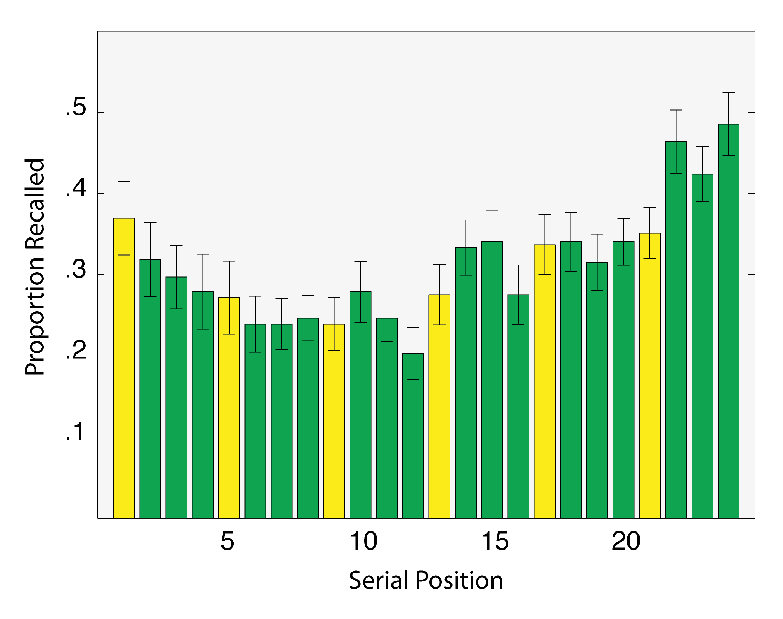
\includegraphics{figures/chapter1_suppfigure1}
\caption{This is the caption}
\end{figure}

\begin{figure}[htbp]
\centering
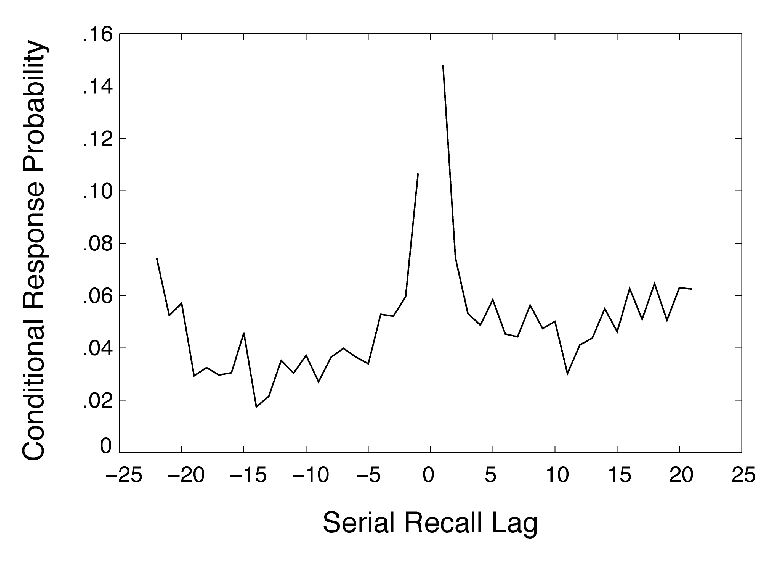
\includegraphics{figures/chapter1_suppfigure2}
\caption{This is the caption}
\end{figure}


\chapter{Chapter 2: Accumulating oscillatory power supports the formation of events in episodic memory}
\section{Abstract}\label{abstract}

GET ABSTRACT FROM CNS

\section{Introduction}\label{introduction}

Our experience of the world can be described as a continuous stream of
sensory information that flows from the external environment into our
brains through our sensory systems. However, empirical studies suggest
that our memories for such experiences are organized according to
contextual features such as perceptual, semantic, temporal and spatial
similarities among the elements of an experience. How do our brains
distill our rich, continuous perceptual experience into meaningful and
manageable units in memory? This question is complex and difficult to
approach because this process likely requires a coordinated interaction
between perception, attention, working memory and long-term memory
processes. While a great deal has been revealed about the neural systems
and processes that contribute to memory formation for individual items
and their associated contexts {[}\textcite{davachi_item_2006};
\textcite{ranganath_neural_2003}; davachi\_multiple\_2003{]}, the
cognitive and neural mechanisms associated with parsing experience into
`mnemonic events' has yet to be fully explored.

Event segmentation theory (EST), a computational/theoretical model of
how the brain parses ongoing experience into events, posits that during
perception the human brain maintains an `event model'. An event model
can be defined as a working memory representation of `what is happening
now' \autocite{kurby_segmentation_2008}. Event models are thought to
contain contextually relevant details of an ongoing experience in order
to generate predictions about future sensory input, which is an
advantageous to an organism in a dangerous and uncertain world. When
there is a substantive change in the perceptual experience (for example,
walking through a door way out of one room and into another) or
predictability breaks down, EST suggests that the previous event model
is abandoned (or perhaps, flushed from working memory) and a new event
model is generated. This process (known as `event segmentation') is
thought to help organize our experience into meaningful units by
integrating information that is perceived to be in the same event, while
keeping across-event information separate.

Emerging evidence suggests that one consequence of event segmentation is
that associative memory for information encoded in distinct events is
reduced relative to information encountered in the same event
\autocites{ezzyat_what_2011}{dubrow_influence_2013}. In these studies,
events are operationalized as temporally adjacent items with overlapping
contextual features. \textcite{ezzyat_what_2011} found that cued recall
performance is reduced for pairs of items that spanned a contextual
shift (or an `event boundary'), and temporal order memory for
across-boundary information is also reduced
\autocite{dubrow_influence_2013}. According to event segmentation
theory, this may occur because the online maintenance of an event model
facilitates the integration of within-event information, and event
boundaries disrupt integration processes. Bolstered by predictions from
EST, these results suggest the existence of a neural mechanism whereby
items are maintained and integrated within an event, but not across
separate events.

In a parallel literature, a number of studies have provided evidence
that sustained and synchronized neural activity (i.e.~neural
oscillations) support the maintenance of information in working memory
\autocites{jensen_frontal_2002}{raghavachari_gating_2001}{hsieh_neural_2011}.
Low frequency oscillatory power (i.e.~Theta: 3/4-8 Hz) during a working
memory delay period has been shown to increase with the number of items
in working memory
\autocites{jensen_frontal_2002}{scheeringa_trial-by-trial_2009}{gevins_high-resolution_1997}{raghavachari_theta_2006},
and the duration of the increase scales with the length of the delay
period \autocite{raghavachari_gating_2001}. Interestingly, recent
evidence suggests that maintenance-related increases in theta power
appear to be specifically related to working memory for temporal
relationships among items, as opposed to the items themselves
\autocite{hsieh_neural_2011}. Thus, theta power increases appear not
only to track the amount of information in working memory, but seems to
be most strongly associated with the maintenance of the associative
relationships among items.

Theta oscillations have also been linked to the successful long-term
memory encoding
\autocites{guderian_medial_2009}{fell_medial_2011}{sederberg_theta_2003}{friese_successful_2013}{summerfield_coherent_2005}{staudigl_theta_2013}{white_theta_2013}{pastotter_distinct_2014}{osipova_theta_2006}{hanslmayr_relationship_2011}
as well as retrieval
\autocites{jacobs_eeg_2006}{addante_prestimulus_2011}{osipova_theta_2006}{bastiaansen_i_2008}{watrous_frequency-specific_2013}.
Numerous studies have found increased theta power for items that are
subsequently remembered as compared to items that are later forgotten
(see above), but others find a mixed or opposite pattern
\autocites{long_subsequent_2014}{burke_synchronous_2013}{greenberg_decreases_2015}{pastotter_distinct_2014}.
Furthermore, a subset of these studies suggest that theta oscillations
are involved in the binding between an item and its context (i.e.~a word
seen in a particular color), rather than indexing memory for an item
alone \autocites{summerfield_coherent_2005}{staudigl_theta_2013}. Taken
together, these data suggest that memory-related theta oscillations may
play a more general role in mnemonic binding or integration (whether
it's an item to its context or an item to another item).

The relationship between lower frequency oscillations and memory has
been studied extensively. Perhaps not surprisingly, most other frequency
bands have also been linked to mnemonic processes in various
experimental designs. The frequency band that has received probably the
least amount of attention with respect to memory is the beta (13-30 Hz)
band. However, there is also some theoretical work suggesting that beta
oscillations may play a role in the maintenance of cognitive states (for
review, see \textcite{engel_beta-band_2010}) and a few papers providing
evidence that beta desynchronization plays a role in episodic memory
encoding
\autocites{hanslmayr_relationship_2011}{hanslmayr_entrainment_2014}{hanslmayr_oscillations_2016}.
While the majority of this evidence comes from studies involving the
maintenance of motor postures (i.e.~holding an arm in a particular
posture) and/or motor plans, a few studies suggest beta may be important
for the maintenance of mnemonic information
\autocites{tallon-baudry_sustained_1999}{tallon-baudry_oscillatory_2001}{tallon-baudry_oscillatory_2004}
as well as the maintenance of an attentional state
\autocite{buschman_top-down_2007}. One recent study found that when
recording from the prefrontal cortex of monkeys performing a 2-item
order maintenance task, beta oscillations increased during the delay
period and beta phase was related to subsequent temporal order memory
success. Thus, beta oscillations may also be involved mnemonic processes
and play a particular role in the maintenance of a cognitive state or
`event model' \autocite{engel_beta-band_2010}.

In this study, we utilized magnetoencephalography (MEG) to ask whether
dynamics in oscillatory power might support the formation of episodic
events. Previous electrophysiological studies of memory have focused on
within-trial spectral and temporal dynamics to examine the time course
of memory-related oscillatory processes. However, relatively fewer
studies have considered the modulation of oscillatory power at longer
timescales (\textgreater{} 5 seconds). In this study, we focused our
analyses on across-trial changes in power to investigate how slower
fluctuations in oscillatory power are modulated by the event structure
in our paradigm and are related to the successful encoding of episodic
events. Guided by models of event segmentation and strong evidence in
support of a relationship between neural oscillations and memory, we
hypothesized that oscillatory power in the theta and beta band would
increase within an event as more information is accumulated and
integrated into the event model. At event boundaries, we predicted that
power would drop significantly as within-event representations might be
flushed from working memory. Finally, we hypothesized that within-event
power accumulation would be related to temporal order memory on a later
test. Specifically, we predicted that successful within-event
integration would be associated with a monotonic increase in power
within an event that might index accumulating within-event information.

\section{Methods}\label{methods}

\subsubsection{Participants}\label{participants}

Twenty healthy right-handed native English speakers (4 males, age range:
21-35, mean age: 28) recruited from New York University and the greater
New York metropolitan area participated in the MEG experiment. The study
was approved by the University Committee on Activities Involving Human
Subjects and all participants gave informed written consent. We excluded
two subjects whose performance on the order memory test was not
significantly different from chance (50\%, using binomial test) and one
subject who did not complete the study due to drowsiness. We excluded
these participants, leaving 17 subjects for the MEG analyses.

\subsubsection{Materials}\label{materials}

Stimuli consisted of 576 gray-scale pictures of objects collected from
various online sources. Colored borders for the objects were generated
by selecting 24 unique colors from a color continuum ranging from
{[}0,0,0{]} to {[}255,255,255{]} RGB values. Colors were chosen to be
maximally distinct from each other. Within the experiment, the order of
the stimuli varied for each subject and color-stimulus pairings were
randomized across subject.

\subsubsection{Encoding}\label{encoding}

During encoding, participants made pleasant/unpleasant decisions on
trial-unique objects that were paired with a colored background frame
(see Figure 2.1). Specifically, participants were instructed to imagine
each object in the color of the background frame and press a button to
indicate whether or not the combination was pleasant. Additionally, we
instructed participants to integrate the objects together by imagining
them interacting with each other. We instructed participants to use this
encoding strategy because it would help them with a later temporal order
memory test. The background color frame remained the same for 6
consecutive trials and then switched to a new color. We operationalized
objects that were studied consecutively in the same color as an `event'
and switches in color as an `event boundary'. There were 6 events
(totaling 36 objects) in each encoding block and 16 encoding/test blocks
across the experiment. Each object was on the screen for 2.5 seconds,
followed by a 2 second inter-trial interval and a .5 second fixation
period. The timing of the task was fixed (i.e.~not jittered).

\subsubsection{Color Memory Test}\label{color-memory-test}

After each encoding block, we tested two types of memory. First, we
tested object-color associative memory. In this test, a previously
studied object appeared in the middle of the screen and two colors
appeared below it. One of the colors was studied with the object (target
color), while the other was a lure color studied in a neighboring event.
Subjects were instructed to indicate which of the two colors was studied
with the object and rate their confidence. Thus, there were four
possible responses during the test: High confidence target, low
confidence target, high confidence lure and low confidence lure. There
were two conditions in the color memory test. The `boundary' condition
consisted of trials that were studied concurrent with a color switch.
The `non-boundary' condition was comprised of trials from the middle of
an event (specifically in the fourth position of an event). The test was
self-paced with a mandatory .5 second fixation period between each test
trial.

\subsubsection{Temporal Order Memory
Test}\label{temporal-order-memory-test}

After the color memory test, there was a temporal order memory test. In
this test, two previously studied objects were presented side by side
without the colored background frame. Participants were asked to
indicate which of the two objects appeared first in the sequence. Like
the color memory test, there were four possible responses (see above).
In the `within-event' condition, objects from the 2nd and 6th
within-event position were presented together and participants were
asked to indicate which came first (position two would be the correct
answer). In the `across-boundary' condition, objects studied in the 5th
position of an event and the 3rd position of the next event were
presented together (position 5 would be the correct answer). Critically,
all tested object pairs were separated by 3 intervening trials during
encoding. Thus, while objects in the `within-event' condition came from
the same event, objects in the `across-boundary' condition were studied
in neighboring events and the amount of elapsed encoding time between
the two test items for the two conditions was identical.

\subsubsection{MEG recordings and data
processing}\label{meg-recordings-and-data-processing}

EG data were recorded using a 157-channel whole-head axial gradiometer
system (KIT, Kanazawa, Japan). Three reference channels seated above the
MEG system were also recorded and used to remove ambient electromagnetic
environmental noise from the data. MEG data were acquired in DC with a
sampling rate of 1000 Hz, a low pass filter at 200 Hz and a notch filter
at 60 Hz to remove line noise. To measure head position, 5
electromagnetic coils were attached to a participant's head during
recording. Coil locations were determined by registering scalp coil
positions with 3D digitized head shape data (software: Source Signal
Imaging, Inc.; hardware: Polhemus, Inc.), which was collected before MEG
recording. The anatomical locations used to register the coils with the
head shape data were the nasion and the left and right periauricular
points. The coils were localized to the MEG sensors at the beginning and
end of the experiment.

MEG data were preprocessed as follows: raw MEG data were loaded into
MATLAB (version 7.10, Mathworks) and malfunctioning channels (average
per subject: \textasciitilde{}2) were immediately removed and
interpolated with the average of its nearest neighbors. Then, data were
denoised using a time-shifted principal components analysis approach
(temporal shift parameter = 100ms), which removed ambient environmental
noise using 3 reference channels \autocite{de_cheveigne_denoising_2007}.
The remaining preprocessing steps utilized the Fieldtrip M/EEG software
package \autocite{oostenveld_fieldtrip:_2010} and custom MATLAB scripts.
The data were band-pass filtered (default settings in eegfilt.m) from
1-100 Hz. Then, the data were epoched from -4 to 4 seconds surrounding
trial onset to assure adequate time for spectral estimation of both pre-
and post-stimulus activity. The epochs were downsampled to 500 Hz to
speed processing time in later steps. Finally, to facilitate
interpretation of topographic plots, we transformed the MEG data from
axial to planar gradient. One advantage of this linear transformation is
that planar signal amplitude is typically largest directly above the
source, whereas axial signal amplitudes are typically maximal on either
side of the neural source of the signal. This transformation was
performed for all topographic analyses, but not the source-space
analyses.

After preprocessing, the MEG data were examined for artifacts. The
artifact rejection approach we took was three-fold: First, excessively
noisy trials and channels were removed using Fieldtrip's visual artifact
rejection `trial summary' feature. Specifically, channels and trials for
which the across-trial variance exceeded 3 standard deviations from the
mean were identified and removed from the analysis. Then, independent
component analysis was implemented to remove components related to eye
blinks, eye movements, and heartbeat-related artifacts. Finally,
remaining trials were visually inspected and epochs containing any
remaining artifacts were removed from the dataset. The group average
proportion of trials removed due to artifacts was
\textasciitilde{}8.6\%.

\subsubsection{Time-Frequency Analyses}\label{time-frequency-analyses}

A time-frequency transformation was applied to each epoch (-4 to 4
seconds, 50 ms sliding window, zero-padded) using a morlet wavelet
approach (number of cycles=6) in Fieldtrip, estimating spectral power
from 1 to 100 Hz in steps of 1Hz. This analysis resulted in
time-frequency spectrograms representing oscillatory power in each
time-frequency-sensor point for each trial and each subject. This
relatively long epoch window allowed us to analyze data during the
`stimulus on' period (0 to 2.5 seconds) as well as the inter-trial
periods (-2.5 to 0 seconds) while avoiding edge artifacts particularly
in the low frequencies. For analyses where power was averaged across the
entire trial, data from the trial N (0 to 2.5 seconds) and the
pre-stimulus period of the next trial (N+1; -2.5 to 0 seconds) were
averaged. This was because we centered the time-frequency analyses on
the onset of each trial.

\subsubsection{Power Accumulation
Analyses}\label{power-accumulation-analyses}

To determine whether oscillatory power increased as a function of within
event position, we adopted a general linear model approach (GLM). For
each trial, we averaged oscillatory power across the entire trial (0 to
5 seconds) for each frequency (1-100 Hz) and each sensor (n=157). We
then set up our `power accumulation' model. The power accumulation model
was simply a mean-centered vector that linearly increased from 1 to 6
within each event and reset back to 1 at event boundaries (see Figure
2.2). Put another way, the accumulation model indexed the within-event
position of each trial. Also included in the GLM was a regressor
modeling the mean signal across the entire experiment as well as a
regressor to account for mean signal differences across the 16 blocks.
We then regressed the power data (separately for each band and sensor)
against this model to obtain a t-statistic representing the fit of the
oscillatory power data to the `accumulation' model. A model fit
statistic (t-value) was obtained for each frequency bin and subject (as
well as each sensor and time point depending upon the analysis).
Finally, to look for reliability of these model fits across subjects, we
performed a group-level one-sample t-test at each frequency bin-sensor
data point.

\subsubsection{Source Localization
Analysis}\label{source-localization-analysis}

Beamformer analysis (DICS; CITATION) was performed to estimate neural
sources of the power accumulation effects. Each subject's data was first
registered to a structural template MPRAGE brain
\autocite{jenkinson_fsl_2012} by aligning anatomical landmarks (nasion,
left/right periauricular points) from the digitized head shape data to
the structural brain image. Then, oscillatory power (for the bands of
interest: delta, theta and beta) was computed in source space for each
trial during the stimulus on period (0-2.5 seconds). We used only the
`stimulus on' periods in this analysis since this time period was the
most significant in the sensor space analyses (see Figure 2.3). The
source-space data were fit to the same power accumulation model
described above, to identify putative generators of the ramping
within-event oscillatory neural activity. Group-level reliability was
then calculated with a one-sample t-test across subjects.

\section{Results}\label{results}

\begin{figure}
  \centering
  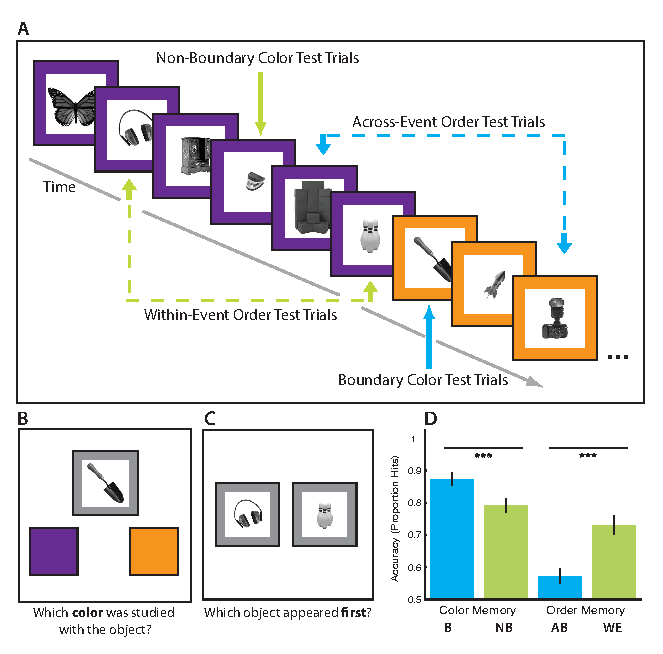
\includegraphics[width=\textwidth]{figures/chapter2_figure1.eps}
  \caption[Schematic of the paradigm and behavioral findings]{\textit{Schematic of the paradigm and behavioral findings.} (A) Participants made pleasantness judgments on trial-unique objects, one at a time, embedded on colored background frames.  After each encoding block, participants performed a color-object memory test (B) and a temporal order test (C).  Plotted in (D) is performance on the object color memory test and the temporal order memory test (B=Boundary condition, NB=Non-boundary condition; AB=Across-boundary condition, WE=Within-Event condition; p<.001).}
  \label{chapter2_figure1}
\end{figure}

\subsubsection{Encoding}\label{encoding-1}

On each encoding trial, participants were instructed to imagine an
object in the color of the background frame and decide if the
combination was pleasant or unpleasant (62\% rated as pleasant).
Encoding task response times (RTs) varied as a function of within-event
position {[}\emph{F}(5,80) = 16.44, \emph{p} \textless{} .0001{]}, where
follow-up pairwise t-tests reveal that RTs to boundary items were
significantly slower than RTs to other positions {[}2-5, all \emph{p}'s
\textless{} .001, corrected for multiple comparisons{]} and there were
no other differences. This boundary-related RT cost replicates a
Experiment 2 from Chapter 1.

\subsubsection{Temporal Order Memory}\label{temporal-order-memory}

After each encoding block, participants were asked to decide which of
two previously studied items occurred earlier in the sequence (see
Methods for more details). We predicted that within-event temporal order
memory would be greater than across-event order memory. Consistent with
our hypothesis, temporal order memory was significantly more accurate in
the within-event condition than the across-boundary condition
{[}within-event condition: \(\mu\) = .73, \(\sigma\) = .12;
across-boundary condition: \(\mu\) = .57, \(\sigma\) = .09; \emph{t}(17)
= 5.56, \emph{p} \textless{} .0001{]}. Critically, the temporal lag
between the retrieval probes in both conditions was fixed at three and
thus, the only difference between conditions was the occurrence of an
intervening event boundary in the across-boundary condition. These data
suggest that event boundaries result in reduced temporal order memory
(relative to within-event temporal order memory), consistent with
previous studies
\autocites{dubrow_influence_2013}{dubrow_temporal_2014}. Next, we tested
whether response times during the temporal order retrieval task varied
by condition. We hypothesized that even when participants make a correct
temporal order response, they might be slower to respond to
across-boundary order test trials as compared to the within-event test
trials. Consistent with this prediction across-boundary test trial RTs
{[}\(\mu\) = 3.79 (s), \(\sigma\) = 1.67{]} were significantly slower
than within-event test trial RTs {[}\(\mu\) = 3.43 (s), \(\sigma\) =
1.22; \emph{t}(17) = 2.36, \emph{p}\textless{}.05{]}. Thus, in addition
to reduced accuracy, when participants made a correct response in the
across-boundary order condition, they were significantly slower.

\subsubsection{Object-Color Memory}\label{object-color-memory}

We hypothesized that object-color memory at event boundaries would be
facilitated relative to object-color memory for trials in the middle of
an event (specifically, in the 4th position of an event). To test this
hypothesis, we probed memory for the object-color association for these
two positions. After each encoding block, we presented a previously
studied object along with a target color (i.e.~that color that was
studied with the word) and a lure color (a color from a neighboring
event). Consistent with our hypothesis, object-color associative memory
was significantly greater at boundaries {[}\(\mu\) = 87.27\%, \(\sigma\)
= 8.41\%{]} then at non-boundaries {[}\(\mu\) = 79.08\%, \(\sigma\) =
9.25\%{]}, suggesting that event boundaries facilitated object-color
binding {[}\emph{t}(17) = 5.54, \emph{p} \textless{} .001{]}. Next, we
asked whether correct responses were speeded in the boundary condition,
relative to the non-boundary condition. We hypothesized that even when
conditions were matched for accuracy, boundary trials would be accessed
more quickly than non-boundary trials. Indeed, correct boundary RTs
{[}\(\mu\) = 2.05 (s), \(\sigma\) = .58{]} were on average half of a
second faster than correct non-boundary RTs {[}\(\mu\) = 2.54 (s),
\(\sigma\) = .84{]}, suggesting that color-object memory on boundary
trials was accessed significantly faster than non-boundary trials
{[}\emph{t}(17) = -4.85, \emph{p} \textless{} .001{]}. Both the temporal
order and color memory findings are consistent with the results
presented in Chapter 1. The remainder of this manuscript will focus on
oscillatory activity during the encoding of events related to the
integration of within-event information.

\begin{figure}
  \centering
  \includegraphics[width=\textwidth]{figures/chapter2_figure2.eps}
  \caption[Within-event power accumulation analyses]{\textit{Within-event power accumulation analyses.} (A) Visual depiction of the ‘accumulation model’.  Oscillatory power was fit to a model that increased linearly within an event and reset at boundaries. (B) Distribution of group-level fits to the accumulation model as a function of frequency (in blue) reveal maximally significant peaks in delta (1), theta (2), and two peaks in beta (3 and 4).  In gray, the average group-level fits to the accumulation model for the 5 ‘out-of-phase’ models.  Dashed line indicates p<.001 significance threshold.  (C) Group-level accumulation model fits were computed for each time-frequency data point separately (averaged across a sensors).  Time-frequency data marked in black were significant at p<.001, cluster threshold p<.001, corrected at p<.05.}
  \label{chapter2_figure2}
\end{figure}

\subsubsection{Oscillatory power increases within
events}\label{oscillatory-power-increases-within-events}

To test our hypothesis that oscillatory power would increase within an
event (i.e.~6 objects studied in with the same color) and drop off at
event boundaries, we adopted a model-based regression approach (Figure
2.2, see Methods for details). For each subject, we fit an
`accumulation' model to the trial-level oscillatory power estimates. As
described in the Methods, the accumulation model was simply a function
that increased linearly within each event (i.e.~6 adjacent items with
the same color background; see Figure 2.2 for visual depiction). Power
was averaged within each trial (0 - 2.5 seconds) and the modulation of
power across trials was fit to the accumulation model. First, we
performed this across-trial regression analysis for each frequency band
separately (1-100 Hz), averaging across all MEG sensors. The results
show well-defined peaks in the distribution of model fits in delta (2
Hz) and theta (7 Hz), as well as two peaks in the beta band (16 and 26
Hz), indicating that these frequency bands significantly fit the
accumulation model {[}\emph{p}'s \textless{} .001, Figure 2.2{]}. In
addition to the parametric statistics, we also performed a permutation
analysis, where for each iteration (n=1000), we shuffled the trial-level
data (within-subject) and refit the model for every subject and then
recomputed the group-level statistics. The result was a null
distribution of group-level model fit significance values for each
frequency band. The non-parametric statistics were very similar to the
parametric tests and each frequency peak (in delta, theta and beta)
remained significant (\emph{p} \textless{} .001). As an additional
control analysis, we recomputed the fits between the power data in each
frequency but shifted the phase of the accumulation model. We predicted
that the model that was `in-phase' with the event structure of our task
would be the most significant, while `out-of-phase' models would not
show a reliable relationship to the data. There were 5 possible
phase-shifted models. None of the 5 out-of-phase models reached
significance in any frequency band at our statistical threshold
(\emph{p} \textgreater{} .001). Thus, the model that was in-phase with
the event structure of the task best fit the data. In summary, power in
delta, theta and beta significantly co-varied with the event structure
of the experiment, suggesting that these bands may play a role in event
formation and segmentation.

\begin{figure}
  \centering
  \includegraphics[width=\textwidth]{figures/chapter2_figure3.eps}
  \caption[Topographic and source space power accumulation analyses]{\textit{Topographic and source space power accumulation analyses.} (A) For the three frequency bands of interest (delta, theta and beta), we computed accumulation model fits for each sensor.  Topographic data were thresholded at p<.001, cluster threshold p<.001, corrected at p<.05.  We then extracted MEG data from sensors that displayed a significant model fit and plotted the group-average z-normalized MEG data across averaged across encoding blocks (in blue).  Each gray line represents the slope of power accumulation within an event (i.e. power across 6 trials within the same event). (B) Results of the source space power accumulation analyses for frequency bands of interest (delta, theta and beta).  Source-space data were thresholded at p<.005.}
  \label{chapter2_figure3}
\end{figure}

\subsubsection{Temporal specificity of power accumulation
effects}\label{temporal-specificity-of-power-accumulation-effects}

Our next analysis aimed to characterize what time periods during each
trial showed the most robust power accumulation effects. One possibility
is that the stimulus-evoked response increase in magnitude across the
event and drive the significant model fits reported above.
Alternatively, if power was gradually increasing across the event, one
might expect the linear increases in power to be present for the
duration of the trial and into the inter-trial interval. For each trial,
we computed a time-frequency spectrogram (-1 to 4 seconds in 50ms bins,
1-100 Hz in 1 Hz bins) and then fit the accumulation model across trials
to each time-frequency data point. This analysis resulted in a single
time-frequency spectrogram (averaged across all MEG sensors), where each
data point represents the fit to the accumulation model at a particular
time point in a particular frequency (Figure 2.2). The result of this
analysis suggests that model fits were maximal during the time that the
stimulus was on the screen, but were also robust in the post-stimulus
time window (after 2.5 seconds when the stimulus was removed from the
screen), suggesting that the power accumulation effects were not driven
by the stimulus-evoked component and not limited to the temporal
interval when the stimulus was on the screen. Thus, these effect do not
appear to be driven by stimulus-evoked activity alone, but rather more
likely reflects cognitive processes evolving at longer timescales
presumably tracking the event structure of the task.

\subsubsection{Spatial specificity of power accumulation
effects}\label{spatial-specificity-of-power-accumulation-effects}

Next, we sought to characterize the topographic distributions of the
within-event power accumulation effects. We limited our analyses to
frequency bands that displayed peaks in the distribution of accumulation
model fits (specifically, the delta, theta and beta bands). We found
that both delta and theta oscillatory accumulation model fits were
significant and maximal over posterior sensors {[}Figure 2.3, \emph{p}
\textless{} .001, cluster threshold: \emph{p} \textless{} .001,
corrected at \emph{p} \textless{} .05{]}. On the other hand, model fits
to beta power were significant in more sensors distributed across most
of the scalp {[}\emph{p} \textless{} .001, cluster threshold: \emph{p}
\textless{} .001, corrected at \emph{p} \textless{} .05{]}.\\
To verify that the within-event power increases that we've characterized
thus far were driven by gradual increases in power within an event that
drops at event boundaries (rather than being driven by another pattern
of activity or alternatively, an artifact of the way we modeled the
data), we extracted power estimates from sensors that showed a
significant fit to the accumulation model. Then, separately for each
frequency band of interest (delta, theta, beta), we averaged the power
data over significant sensors. This resulted in a single time course of
oscillatory power for each frequency band across the entire duration of
the experiment. To increase our signal to noise ratio, we downsampled
our time courses, binning the power time courses into 500 millisecond
chunks and and averaging. We also averaged over all 16 encoding blocks
(and across subjects). Plotted in Figure 2.3 is the time course of
oscillatory power for delta, theta and beta across an entire encoding
block (i.e.~36 trials / 6 events). Each gray line represents the slope
of the power increase within an event. Visual inspection of the time
courses clearly display accumulating power within an event that drops at
the event boundaries in all three frequency bands of interest. This
analysis provides compelling evidence that oscillatory power in the
delta, theta and beta bands tracks the event structure in our task.

\subsubsection{Ruling out potential
confounds}\label{ruling-out-potential-confounds}

We performed a series of control analyses to consider possible confounds
and alternative explanations. First, we noted that oscillatory power
appeared to increase not only within an event, but also across the
duration of a study block (see Figure 2.3). In other words, we observed
power increases within an event but also power increases over a block of
36 trials. To test whether our accumulation model analyses were driven
by power changes across an encoding block (rather than power increases
within an event), we regressed out block-level linear trends and
recomputed the model fits on the residuals of this regression. This did
not account for the results, as the effects remained statistically
robust (STATS). We also noticed that overall power in the first event of
a block was notably lower than the rest of the events. Thus, we removed
the first event from the analyses and recomputed the accumulation model
analyses. Again, this did not change the pattern of results (STATS).
Another possibility is that evoked responses (i.e.~ERPs) might
contribute to this accumulation effect, rather than induced oscillatory
activity. To rule out this possibility, we subtracted out the average
evoked response from each trial and recomputed the accumulation
analysis. This did not change the results, suggesting that trial-evoked
responses did not explain the power accumulation effects. Finally, we
tested whether the accumulation effects were sensitive to baseline
correction. We baseline corrected each trial to the pre-stimulus period
(-1000 to -500 ms). Interestingly, the effects were eliminated (STATS),
which is consistent with the idea that the power accumulation effects
were not limited to the periods when the stimulus was on the screen, but
may also exist in the pre-stimulus periods. This interpretation is also
supported by the fact that the pre-stimulus oscillatory power in delta,
theta and beta fits the accumulation model (See Figure 2.3). Together,
these data provide compelling evidence that oscillatory power in delta,
theta and beta increases within an event and drops at event boundaries,
and that this dynamic pattern likely reflects cognitive processes that
evolve over the timescale of a temporally-extended episodic experience.

\subsubsection{Source Localization of the power accumulation
effects}\label{source-localization-of-the-power-accumulation-effects}

The purpose of the next analysis was to 1) localize the source(s) of
within-event power accumulation signals and 2) test whether different
frequency bands localized to different brain areas. To achieve this, we
utilized a beamforming procedure (see Methods for details) to estimate
oscillatory source power for each trial in three frequency bands of
interest (delta, theta and beta). Given that we observed the strongest
accumulation effects during the `stimulus on' period in the trial (0 to
2.5 seconds), we averaged power across this epoch for each trial. We
then fit the source space power data to the same power accumulation
model as described above. We (primarily) focused our analyses on the
peaks in the frequency distribution of accumulation model fits (as shown
in Figure 2.2), since these were the frequency bands that best fit our
power accumulation model. Delta (2 Hz) power accumulation was localized
to the right hippocampus and right cerebellum. High theta (7 Hz) was
localized to the right paracentral lobule. Low beta (16 Hz) localized to
the right MTL, right inferior frontal junction, and left premotor
cortex. High beta (26 Hz) localized to the cerebellum bilaterally, left
lateral occipital complex (LO) and right parietal cortex. Finally, given
recent evidence suggesting that low theta (\textasciitilde{}3-4 Hz) is
related to episodic memory in humans (Watrous et al; Jacobs et al), we
source localized low theta (4 Hz) power accumulation. This analysis
localized low theta power accumulation to the left hippocampus/MTL, the
left cerebellum (vermis VIIIa), and the left superior frontal sulcus.

Visual inspection revealed overlap in the source localization for theta
(4 Hz) and low beta (16 Hz). To quantify this overlap, we ran a
conjunction analysis (joint \emph{p} \textless{} .0001, individuals maps
thresholded at \emph{p} \textless{} .01). This analysis revealed that
source localization for beta and theta overlapped in the left MTL and a
left insular region (Figure 2.3). Thus, while low frequency power
accumulation (4 Hz and lower) was localized primarily to the hippocampus
and MTL, higher frequency beta power accumulation was localized to
frontal and parietal regions (as well as MTL and LO) and there was
overlap between the theta and beta source localization in the left MTL
and insula.

\begin{figure}
  \centering
  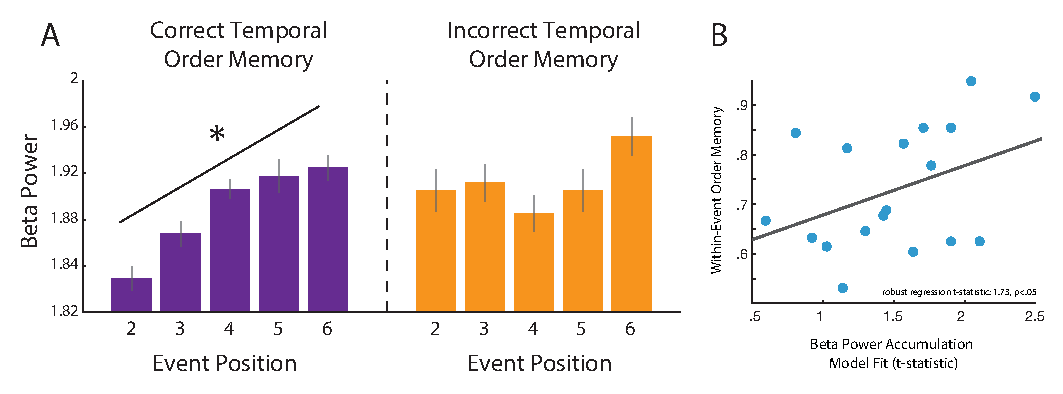
\includegraphics[width=\textwidth]{figures/chapter2_figure4.eps}
  \caption[Power accumulation and temporal order memory]{\textit{Power accumulation and temporal order memory.} (A) Average beta power as a function of event position plotted separately for correct (purple) and incorrect (orange) temporal order memory.  The linear trend significant for correct order memory (p<.001). Error bars represent standard error of the mean. (B)  Correlation between beta power accumulation model fits and within-event temporal order memory across subjects.}
  \label{chapter2_figure4}
\end{figure}

\subsubsection{Power accumulation and subsequent temporal order
memory}\label{power-accumulation-and-subsequent-temporal-order-memory}

In the next set of analyses, we asked whether increasing power within an
event was related to successful temporal order memory. We focused our
analyses on sensors that showed a significant fit to the accumulation
model in our three bands of interest (delta, theta and beta). For each
trial, we extracted power from sensors that displayed significant
accumulation model fits (averaging across sensors). Then, we binned
trials by the within-event trial position (1-6) and also by later
within-event temporal order memory. To test for differences in the
pattern of power accumulation between hits and misses, we performed
repeated-measures ANOVAs testing for a significant linear trend within
an event. We excluded boundary trials (i.e.~position 1) from this
analysis, as they were not part of the temporal order memory decision
(within-event temporal order judgment was on trials 2 and 6). In all
three bands, we observed a significant linear trend for events where
order was later correct {[}delta: \emph{F}(1,17) = 19.88, \emph{p}
\textless{} .001; theta: \emph{F}(1,17) = 18.82, \emph{p} \textless{}
.001; beta: \emph{F}(1,17) = 29.83, \emph{p} \textless{} .001{]}, but
not for incorrect events {[}delta: \emph{F}(1,17) = .294, \emph{p}
\textgreater{} .1; theta: \emph{F}(1,17) = 1.53, \emph{p} \textgreater{}
.1; beta: \emph{F}(1,17) = 1.95, \emph{p} \textgreater{} .1{]}. For beta
(but not delta or theta; \emph{p}'s \textgreater{} .2), there was also a
significant position by memory interaction {[}\emph{F}(4,68) = 3.11,
\emph{p} = .02{]} and a trending interaction of the linear contrast
{[}\emph{F}(4,68) = 3.76, \emph{p} = .069{]}. Since differences in trial
numbers between conditions can influence estimates of oscillatory power,
we performed an additional sub-sampling analysis where for each
iteration (n=1000) we randomly selected a subsample of trials to match
the number of trials between conditions. Since every subject had more
trials for the remember condition, this analysis essentially matched the
number of trials in the `hits' bin to the number of trials in the
`misses' bin. We performed this analysis for all subjects and then
averaged across the iterations and recomputed our statistics. This
analysis suggested that differences in trial numbers going into the
power estimates did not account for differences in the linear trend as a
function of conditions {[}linear trend for hits: delta: \emph{F}(1,17) =
20.74, \emph{p} \textless{} .001; theta: \emph{F}(1,17) = 18.24,
\emph{p} \textless{} .001; beta: \emph{F}(1,17) = 30.19, \emph{p}
\textless{} .001; linear trend for misses same as reported above{]}. The
significant memory by position interaction {[}\emph{F}(1,17) = 3.05,
\emph{p} = .02{]} and trending interaction in beta power of the linear
contrast (hits vs.~misses) was also replicated {[}\emph{F}(1,17) = 3.78,
\emph{p} = .07{]}. In summary, oscillatory power (in delta and theta,
but most robustly in beta) during successful order encoding linearly
increased over trials within an event and this linear pattern was not
present when temporal order later incorrect.

Notably, this linear accumulation effect was not driven by overall
greater power for temporal order correct events. In fact, the opposite
pattern was true: trials for which temporal order was later tested
actually showed greater oscillatory power for misses as compared to hits
{[}delta, 2nd position: \emph{t}(17) = -2.12, \emph{p} \textless{} .05;
delta, 6th position: \emph{t}(17) = -2.09, \emph{p} = .051; theta, 2nd
position: \emph{t}(17) = -2.03, \emph{p} = .057; theta, 6th position:
\emph{t}(17) = -2.28, \emph{p} \textless{} .05; beta, 2nd position:
\emph{t}(17) = -2.26, \emph{p} \textless{} .05; no other significant
differences{]}. Thus, the pattern of power accumulation across an event
was predictive later order memory, but the absolute magnitude of power
(in all three bands) was predictive of later mnemonic errors.

\subsubsection{Leveraging across-subject variability in power
accumulation model
fits}\label{leveraging-across-subject-variability-in-power-accumulation-model-fits}

Next, we tested the prediction that variability in the extent to which
individual participants fit the accumulation model would be related to
within-event temporal order memory. Specifically, we predicted that
subjects whose oscillatory power dynamics better fit the accumulation
model would show better within-event temporal order memory as compared
to subjects that poorly fit the model. We limited our analyses to the
delta, theta and beta bands averaging across the sensors that
significantly fit the accumulation model (at the group-level).
Consistent with our prediction, beta accumulation model fits were
positively correlated with within-event order memory {[}Figure 2.4;
robust regression: \emph{t}(16) = 1.73, \emph{p} \textless{} .05,
one-tailed{]}. There was no such relationship in delta or theta
{[}\emph{p}'s \textgreater{} .1{]}. It's worthwhile to note that if when
we analyzed the data with a stricter statistical threshold (that is,
averaging across sensors that exceeded a p\textless{}.0001 threshold),
the correlation became stronger {[}robust regression: {[}\emph{t}(16) =
2.16, \emph{p} \textless{} .05{]}. In summary, participants whose beta
power dynamics better fit the event accumulation model showed relatively
better temporal order memory.

\begin{figure}
  \centering
  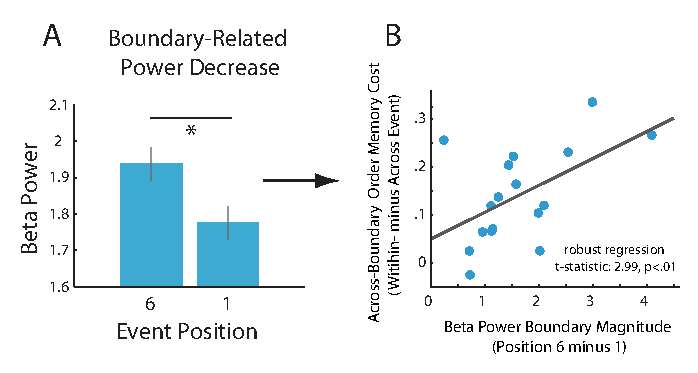
\includegraphics[width=\textwidth]{figures/chapter2_figure5.eps}
  \caption[Boundary-related power decreases and temporal order memory.]{\textit{Boundary-related power decreases and temporal order memory.} (A) Average boundary-related drop in beta power from position 6 trials to position 1 trials averaged across sensors that displayed significant fit to accumulation model (p<.001).  (B) Across-subject correlation between magnitude of the drop in beta power (position 6 minus position 1) and the difference in within-event and across-boundary temporal order memory.}
  \label{chapter2_figure5}
\end{figure}

\subsubsection{Boundary-related decreases in power predict
across-boundary order memory
cost}\label{boundary-related-decreases-in-power-predict-across-boundary-order-memory-cost}

The previous analyses were aimed to identify oscillatory activity that
followed a linearly increasing pattern within an event. In this next set
of analyses, we test the hypothesis that event boundaries result in a
significant drop in power. Although we've already provided evidence that
oscillatory activity significantly fits our within-event accumulation
model, it remains possible that this is pattern is not driven by a
significant drop in power at boundaries. For instance, a linear trend
(within an event) could exist in the data without any significant
differences between positions. To test this, we extracted delta, theta
and beta power data from sensors showing significant accumulation model
fits (averaging across sensor) for trials in position 6 (i.e.~the last
trial before a boundary) and trials in position 1 (the first trial after
a boundary). We hypothesized that power would be significantly higher
for trials in the last position of an event compared to trials in the
first position of an event. We found this to be true for all three bands
{[}delta: \emph{t}(17) = 4.85, \emph{p} \textless{} .001; theta:
\emph{t}(17) = 5.05, \emph{p} \textless{} .001; beta: \emph{t}(17) =
7.52, \emph{p} \textless{} .001{]}. While this analysis is not entirely
independent from within-event power accumulation analyses described
earlier, it provides corroborating evidence that event boundaries result
in a drop in a significant oscillatory power.

Next, we tested the hypothesis that boundary-related decreases in power
would influence temporal order memory organization. Our logic was the
following: if power decreases at event boundaries represent flushing of
event content from working memory, then subjects who displayed larger
boundary-related decrease in oscillatory power might also show larger
boundary-related cost in temporal order memory. For our three bands of
interest, we extracted power from sensors showing significant
accumulation model fit from trials in position 6 (i.e.~the last trial in
an event) and position 1 (i.e.~the first trial after a boundary) and
computed a difference score (position 6 minus position 1 power). We
hypothesized that this difference score might represent an individual's
neural sensitivity to event boundaries. Then, for each subject, we
computed a boundary-related order memory cost index by subtracting
overall across-boundary order memory from within-event order memory.
This difference score served as a proxy for how much the boundaries
reduced across-event temporal order memory (relative to within-event
order memory). We removed one outlier whose behavioral difference score
was 2.37 standard deviations from the mean. We found that the
boundary-related decrease in beta power (but not theta or delta,) was
correlated with the magnitude of the across-boundary order memory cost
{[}Figure 2.5; robust regression: \emph{t}(16) = 2.99, \emph{p}
\textless{} .01{]}. This correlation remained significant when including
the outlier subject in the analysis {[}robust regression: \emph{t}(17) =
2.58, \emph{p} \textless{} .05{]}. We did not observe this pattern in
delta or theta (both \emph{p}'s \textgreater{} .4). When considering the
within-event and across-event trials alone, there was trending effect
for within-event {[}robust regression: \emph{t}(17) = 1.66, \emph{p} =
.06{]} and no effect for across-event {[}robust regression: \emph{t}(17)
= .83, \emph{p} = .11{]}. Thus, the subtraction likely acted as a
baseline to remove gross across-subject memory differences that might
have dampened this relationship. This finding suggests that the
magnitude of drop in beta power at event boundaries is related to the
impact of event boundaries on temporal order memory.

\section{Discussion}\label{discussion}

In this study, we recorded oscillatory brain activity during the
encoding of temporally extended experiences and found that temporal
dynamics in delta, theta and beta power tracked the event structure in
our experiment. Specifically, oscillatory power accumulated within an
event, or a sequence of 6 adjacent trials with a shared background
color, and then dropped sharply at boundaries between events. Moreover,
linear increases in power within each event were related to temporal
order memory success, suggesting that these frequency bands (delta,
theta and beta) may play an important role in the organization of
temporally extended memories. These findings contribute to a growing
body of evidence suggesting that neural oscillations play a prominent
role in the formation of episodic memories. Furthermore, our unique
across-trial regression approach to the MEG data highlights the
importance of considering oscillatory dynamics across longer time scales
than what has been typical in the literature.

\subsubsection{Delta/Theta oscillations and temporal memory
formation}\label{deltatheta-oscillations-and-temporal-memory-formation}

The pattern of accumulating theta power within an event is consistent
with prior research demonstrating that increases in theta power are
correlated with working memory load
\autocites{jensen_frontal_2002}{raghavachari_gating_2001}{raghavachari_theta_2006}{hsieh_neural_2011}{scheeringa_trial-by-trial_2009}{gevins_high-resolution_1997}.
Furthermore, a recent EEG study found that (frontal) theta power was
greater during the maintenance of temporal order information as compared
to item maintenance alone \autocite{hsieh_neural_2011}. In the current
study, subjects may be accumulating/maintaining within-event item
representations as an event unfolds. If that is the case, then one might
expect theta power to increase with each additional maintained item (as
working memory load increases). This is exactly the pattern of results
that we observed. Moreover, theta power accumulated specifically when
the order of the items within the event was successfully encoded (and
not when temporal order was incorrect), suggesting that dynamic
increases in theta power across an event may support temporal order
encoding. One interpretation of this pattern is that accumulating theta
power within an event is a by-product of neural processes supporting the
maintenance of multiple items in working memory. Neural representations
of items that are co-active in working memory might become associatively
bound to one another, which could support the recovery of temporal
information on a later test, and explain why accumulating theta power is
related to temporal order memory success. This interaction between a
working memory `buffer' and long-term associative memory is predicted by
memory models that posit that items may become associatively bound in
long-term memory via a `buffer'-like process active during encoding
\autocite{lehman_buffer_2013}.

There is a good deal of evidence now that theta oscillations also play a
role in long-term memory encoding
\autocites{guderian_medial_2009}{fell_medial_2011}{sederberg_theta_2003}{friese_successful_2013}{summerfield_coherent_2005}{staudigl_theta_2013}{white_theta_2013}{pastotter_distinct_2014}{osipova_theta_2006}{hanslmayr_relationship_2011},
and some recent work has argued that theta oscillations may play a more
specific role in associative binding
\autocites{hsieh_neural_2011}{summerfield_coherent_2005}{staudigl_theta_2013}.
\textcite{summerfield_coherent_2005} found that successful word-color
associative memory was accompanied by an increase in frontal theta
power, as well as an increase in frontal-posterior theta coherence. In
another relevant study, \textcite{staudigl_theta_2013} recorded
oscillatory activity while subjects encoded words that were superimposed
on a background movie. Then, they test memory for the words, where some
trials were presented intact (same word, same movie) while other trials
were rearranged (same word, different movie). Interestingly, for intact
test trials they found that greater theta power during encoding was
predictive of item memory. However, for rearranged test trials, the
reverse pattern (i.e.~relatively less theta power during encoding) was
predictive item memory. This suggests that theta power during encoding
indexes item-context binding, since presumably greater item-context
binding would facilitate retrieval in the intact condition, but not in
the rearranged condition. Taken together, these results are consistent
with the idea that theta oscillations may be an index of neural
processes generally supporting associative binding, whether its
within-trial (i.e.~item-context) or across multiple trials
(i.e.~item-item).

Our source analyses suggest that delta and theta power accumulation
appear to be localized to the left hippocampus and right medial temporal
lobes (MTL), respectively. This is consistent with previous research
that has shown that theta oscillations in the MTL appear to play a
critical role in successful memory encoding
\autocites{guderian_medial_2009}{fell_medial_2011}{sederberg_theta_2003}{friese_successful_2013}{summerfield_coherent_2005}{staudigl_theta_2013}{white_theta_2013}{pastotter_distinct_2014}{osipova_theta_2006}{hanslmayr_relationship_2011}.
While some caution is warranted due to the difficult problem of deep
source localization
\autocites{attal_assessment_2013}{mills_techniques_2012}{quraan_detection_2011},
given the robust literature on MTL contributions to memory encoding
paired with the localization results here, we hypothesize that the
within-event delta/theta power accumulation effects we observed in this
study are indeed generated by MTL structures. Future studies could
utilize convergent techniques with higher spatial resolution
(i.e.~intracranial EEG) to validate this localization.

\subsubsection{The Role of Beta Oscillations in the Maintenance of the
Status
Quo}\label{the-role-of-beta-oscillations-in-the-maintenance-of-the-status-quo}

In addition to accumulating theta power, we also found a robust
relationship between accumulating beta power and temporal order memory
within events (Figure 2.4). Like theta power, accumulating beta power
within an event was predictive of temporal order memory success.
Furthermore, subjects who showed larger boundary-related drops in beta
power also had better within- vs.~across-event temporal order memory,
suggesting that beta power dynamics have bearing on memory organization.

In a review of the literature, \textcite{engel_beta-band_2010} propose
that beta oscillations might index the `maintenance of the status quo'.
This theory was primarily inspired by research in the motor domain which
has shown that beta power is elevated during sustained motor operations
(i.e.~holding a posture) and decreases during voluntary movements
\autocites{baker_oscillatory_2007}{sanes_oscillations_1993}{baker_coherent_1997}{kilner_task-dependent_1999}{klostermann_task-related_2007}{chakarov_beta-range_2009}.
The authors suggest that if beta oscillations index the maintenance of a
particular motor state, then they may also be elevated during the
maintenance of a cognitive set (and in other situations of high levels
of endogenous attention) and decrease in the face of novel or unexpected
events. Our results fit well within this framework: we found that beta
oscillations increased monotonically as the event unfolded, and rapidly
dropped at event boundaries (i.e.~when the background changed to a new
novel color). Bolstered by this theoretical work, we speculate that the
beta oscillations we observed here might index the maintenance of a
`cognitive set', or perhaps an `event model', a construct that is
central to event segmentation theory
\autocites{zacks_event_2001}{kurby_segmentation_2008}{zacks_human_2001}.

Beta oscillations have also been directly linked with successful memory
encoding. In a series of intriguing studies, Hanslmayr and colleagues
found that beta desynchronization in the frontal cortex is predictive of
subsequent memory and is also positively correlated with BOLD
activity\autocite{hanslmayr_relationship_2011}. Furthermore, the authors
found that entrainment of the frontal cortex to the beta frequency (but
not theta or alpha entrainment) during encoding selectively impaired
later memory \autocite{hanslmayr_entrainment_2014}. A possible
explanation for this finding is that beta desynchronization may actually
lead to a richer, more unique neural representation (REFS). This
prediction stems from the idea that theoretically, desynchronized brain
activity has a higher information capacity than synchronized activity
\autocite{hanslmayr_oscillations_2016}. Connecting this idea to the
current work, we speculate that accumulating beta power (i.e.~increases
in synchronized activity) may represent the maintenance of a prior
cognitive set (or event model). At event boundaries, when the background
is updated to a novel color, the sharp drop in beta power may reflect
bottom-up processing of novel perceptual information, which may require
relatively greater processing bandwidth. Thus, while beta power
accumulation may be beneficial to forming associative relationships
among a group of items, at the same time greater beta power may be
detrimental to encoding in scenarios where item distinctiveness is
important for memory. Future work should directly test this tentative
hypothesis.

While low frequency power accumulation was localized to MTL structures,
beta power accumulation was localized to regions including the frontal
and parietal cortex. Prior studies have found that synchronized beta
activity between frontal and parietal regions increases under conditions
of high top-down endogenous attention \autocite{buschman_top-down_2007}.
Thus, the observed increase in beta power within an event could reflect
an increase in exogenous attention necessary to maintain accumulating
items in working memory. Thus, at boundaries, the drop in beta power
could reflect a shift from endogenous to exogenous attention.

Finally, we observed overlap in the source localization of theta and
beta in the medial temporal lobe (as well as the insula). Both theta and
beta have been observed in medial temporal lobe structures. Empirical
data and computational models support the idea that while higher
frequency bands (such as gamma) can be used for relatively local neural
computations, it's possible for distal brain regions to synchronize at
lower frequencies (\textless{}gamma) \autocite{kopel}. Thus, both of
beta and theta in the hippocampus could be involved in the integration
of representations that are distributed across different brain regions
in the service of episodic memory encoding. Future work should address
if and how these frequencies might interact.


\chapter{Chapter 3: Episodic sequence memory is supported by a theta-gamma phase code}
\section{Abstract}\label{abstract}

The meaning we derive from our experiences is not a simple static
extraction of the elements but, rather, is largely based on the order in
which those elements occur. Influential theoretical models propose that
the encoding of sequences of elements (or items) may be supported by
interactions between high and low frequency brain rhythms, such that
items within an episode are represented by neural cell assemblies firing
at higher frequencies (i.e.~gamma) and their relative sequential order
is coded by the specific timing of firing with respect to a slower
frequency rhythm (i.e.~theta). Using magnetoencephalography (MEG) to
record neural oscillations during episodic sequence memory formation in
humans, we provide evidence that items in different ordinal positions
within a sequence exhibit relatively greater gamma power along distinct
phases of an underlying theta oscillation. Furthermore, this segregation
is related to successful memory for the order of the items. These
results provide compelling evidence that memory for order, a core
component of an episodic memory trace, capitalizes on the seemingly
ubiquitous physiological mechanism of theta-gamma phase-amplitude
coupling.

\section{Introduction}\label{introduction}

While many aspects of our cognition and behavior, including language
processing, spatial navigation and episodic memory, share the
requirement to represent, encode and retrieve temporal sequences of
events, how the brain accomplishes this is still not well understood. It
is has been known for decades that two stimuli that activate
interconnected neurons can result in long-term potentiation (LTP) of the
bridging synapse \autocite{bliss_long-lasting_1973}, thus supporting an
association between the two, and compelling new research has provided
causal evidence for a link between LTP and associative memory formation
\autocite{nabavi_engineering_2014}. However, the model of long-term
potentiation in its current form is not viable for stimuli (or neurons)
whose activation is separated by more than \textasciitilde{}300 ms, and
unarguably, much of what we encode and remember is separated by temporal
gaps at least an order of magnitude large than this. Thus, a central
issue in understanding temporal sequence learning is how the brain can
bridge and relate stimuli that are encountered across seconds or
minutes.

To deal with this conundrum, mechanistic models of sequence encoding
posit that the temporal coding of sequences can be supported by neural
oscillations
\autocites{lisman_storage_1995}{jensen_hippocampal_1996}{lisman_-_2013}{jensen_physiologically_1996}{koene_first-first-out_2007},
or rhythmic fluctuations in neuronal excitability (see
\textcite{buzsaki_neuronal_2004} for review). One influential model of
sequence encoding \autocites{lisman_storage_1995}{lisman_-_2013}
hypothesizes that individual items are represented by largely
non-overlapping neural cell assemblies that, when activated, fire in
high frequency bands (i.e.~gamma: \textgreater{}30 Hz), while the
relative sequential order of those items is coded in a temporally
segregated manner along the phase of an underlying slower rhythm
(i.e.~theta: \textasciitilde{}3-8 Hz). It follows then that during the
encoding of a sequence, the current item is represented and encoded by
transient higher frequency activity, while the relative position of each
item in a sequence may be coded by the relative phase of a lower
frequency oscillation (referred to as `phase coding'). Theoretically,
phase coding allows the temporal segregation of activity supporting
individual items that are encountered at different times across an
experience, and critically may also permit temporally extended
experiences to be represented in a time-compressed manner
\autocite{jensen_physiologically_1996} (\textasciitilde{}100-300 ms
cycles of neuronal activity).

There is ample evidence that modulation of gamma power by theta phase
(i.e.~phase-amplitude coupling or `PAC') is important for learning and
memory formation
\autocites{axmacher_cross-frequency_2010}{tort_thetagamma_2009}{friese_successful_2013}{fuentemilla_theta-coupled_2010}[gamma\_2014]{lega_slow-theta}
as well as other cognitive processes
\autocites{canolty_high_2006}{giraud_cortical_2012}{szczepanski_dynamic_2014}.
However, to date, there is little evidence that theta phase coding, or
the segregation of item-specific neural assemblies on distinct phases of
an underlying theta oscillation, serves as a mechanism for human
sequence memory encoding. We set out to test this fundamental question
by presenting participants with six-item sequences each consisting of
pictures of trial-unique objects that were embedded on a repeating
background colored frame (Figure 1a) while recording brain activity
using magnetoencephalography (MEG). The colored frame defined each
six-item sequence as the color switched every six trials. We later
tested participants sequence memory by asking them to recognize the
correct order of two previously presented objects during retrieval.
Thus, we could ask whether gamma power associated with each item in a
sequence (positions 1-6) is relatively biased towards distinct phases of
theta (i.e.~phase coding). Importantly, we also assessed whether theta
phase coding was behaviorally relevant by examining phase coding effects
during both successful and unsuccessful temporal order encoding.

\section{Methods}\label{methods}

\subsubsection{Participants}\label{participants}

Twenty healthy right-handed native English speakers (4 males, age range:
21-35, mean age: 28) recruited from New York University and the greater
New York metropolitan area participated in the MEG experiment. The study
was approved by the University Committee on Activities Involving Human
Subjects and all participants gave informed written consent. We excluded
two subjects whose performance on the order memory test was not
significantly different from chance (50\%, using binomial test) and one
subject who did not complete the study due to drowsiness. We excluded
these participants, leaving 17 subjects for the MEG analyses.

\subsubsection{Materials}\label{materials}

Stimuli consisted of 576 gray-scale pictures of objects collected from
various online sources. Some examples of stimuli can be seen in the main
text (Figure 1). Colored borders for the objects were generated by
selecting 24 unique colors from a color continuum ranging from
{[}0,0,0{]} to {[}255,255,255{]} RGB values. Colors were manually chosen
to be maximally distinct from each other.

\subsubsection{Design and Procedure}\label{design-and-procedure}

\emph{Encoding}. During encoding, participants made pleasant/unpleasant
decisions on trial-unique objects that were paired with a colored
background frame. Specifically, participants were instructed to imagine
each object in the color of the background frame and press a button to
indicate whether or not the combination was pleasant. We chose to use
this encoding task to encourage participants to associate the color and
object, since attention to the context (i.e.~color) was critical to our
hypothesis. To promote successful temporal order memory, we additionally
instructed participants to associate neighboring objects together by
imagining them interacting with each other. Subjects were instructed to
perform this task irrespective of the color changes between some of the
items. Pilot data indicated that this instructional manipulation was
critical to achieving above chance temporal order memory performance in
a majority of our participants.

During the encoding task, the background color frame remained the same
for 6 consecutive trials (i.e.~a `sequence') and then switched to a new
color. There were 6 sequences (totaling 36 objects) in each encoding
block and 16 encoding/test blocks across the experiment. Each object was
on the screen for 2.5 seconds, followed by a 2 second inter-trial
interval (ITI) and a .5 second fixation period. The timing of the task
was fixed (i.e.~not jittered). During the ITI and fixation period, the
color frame remained on the screen.

\emph{Temporal order memory test.} After each study block, we tested
temporal order memory. We used this temporal order test as a proxy for
probing intact sequence memory. In this test, two previously studied
objects were presented side by side (with the previously colored
background frame now gray). Participants were asked to indicate which of
the two objects appeared first (earlier) in the sequence and rate their
confidence using a 4 alternative forced choice design. Thus, there were
four possible responses during the test: high confidence correct order,
low confidence correct order, high confidence incorrect order and low
confidence incorrect order. The tested objects always occurred in the
2nd and 6th position within a sequence and all tested object pairs were
separated by 3 intervening trials during encoding. The test was
self-paced with a mandatory .5 second fixation period between each test
trial.

\subsubsection{MEG recordings and data
processing}\label{meg-recordings-and-data-processing}

MEG data were recorded using a 157-channel whole-head axial gradiometer
system (KIT, Kanazawa, Japan). Three reference channels seated above the
MEG system were also recorded and used to remove ambient electromagnetic
environmental noise from the data. MEG data were acquired in DC with a
sampling rate of 1000 Hz, a low pass filter at 200 Hz and a notch filter
at 60 Hz to remove line noise. To measure head position, 5
electromagnetic coils were attached to a participant's head during
recording. Coil locations were determined by registering scalp coil
positions with 3D digitized head shape data (software: Source Signal
Imaging, Inc.; hardware: Polhemus, Inc.), which was collected before MEG
recording. The anatomical locations used to register the coils with the
head shape data were the nasion and the left and right periauricular
points. The coils were localized to the MEG sensors at the beginning and
end of the experiment.

MEG data were preprocessed as follows: raw MEG data were loaded into
MATLAB (version 7.10, Mathworks) and malfunctioning channels (average
per subject: \textasciitilde{}2) were immediately removed and
interpolated with the average of its nearest neighbors. Then, data were
denoised using a time-shifted principal components analysis approach
(temporal shift parameter = 100ms), which removed ambient environmental
noise using 3 reference channels \autocite{de_cheveigne_denoising_2007}.
The remaining preprocessing steps utilized the Fieldtrip M/EEG software
package \autocite{oostenveld_fieldtrip:_2010} and custom MATLAB scripts.
The data were band-pass filtered (default settings in eegfilt.m) from
1-100 Hz. Then, the data were epoched from -4 to 4 seconds surrounding
trial onset to assure adequate time for spectral estimation of both pre-
and post-stimulus activity. The epochs were downsampled to 500 Hz to
speed processing time in later steps. Finally, to facilitate
interpretation of topographic plots, we transformed the MEG data from
axial to planar gradient. One advantage of this linear transformation is
that planar signal amplitude is typically largest directly above the
source, whereas axial signal amplitudes are typically maximal on either
side of the neural source of the signal. This transformation was
performed for all topographic analyses, but not the source-space
analyses.

After preprocessing, the MEG data were examined for artifacts. The
artifact rejection approach we took was three-fold: First, excessively
noisy trials and channels were removed using Fieldtrip's visual artifact
rejection `trial summary' feature. Specifically, channels and trials for
which the across-trial variance exceeded 3 standard deviations from the
mean were identified and removed from the analysis. Then, independent
component analysis was implemented to remove components related to eye
blinks, eye movements, and heartbeat-related artifacts. Finally,
remaining trials were visually inspected and epochs containing any
remaining artifacts were removed from the dataset. The group average
proportion of trials removed due to artifacts was
\textasciitilde{}8.6\%.

\subsubsection{Time-Frequency Power
Analyses}\label{time-frequency-power-analyses}

A time-frequency analysis was performed for each epoch (-4 to 4 seconds,
50 ms sliding window, zero-padded) using a morlet wavelet approach
(number of cycles=6), estimating spectral power from 1 to 100 Hz in
steps of 1 Hz. This analysis resulted in time-frequency spectrograms
representing oscillatory power for each time-frequency-sensor point for
each trial and each subject. This relatively long epoch window allowed
us to analyze data during the `stimulus on' period (0 to 2.5 seconds) as
well as the inter-trial periods (-2.5 to 0 seconds) while avoiding edge
artifacts particularly in the low frequencies.

\subsubsection{Cross-Frequency Coupling
Analyses}\label{cross-frequency-coupling-analyses}

Phase-amplitude cross-frequency coupling (PAC) was estimated as follows
for each trial for each sensor and subject. The algorithm to compute the
PAC `modulation index' (referred to as MI or coupling values/estimates)
was taken from \textcite{tort_measuring_2010}. First, to compute gamma
amplitude, raw MEG time-series (for each trial/sensor) was filtered from
70-100 Hz, which was determined by frequencies that showed a peak in the
spectral power distribution (Supplemental Figure 1). The envelope was
then computed by taking the absolute value of the Hilbert Transform of
the filtered time-series. To compute theta phase, the raw data was
filtered from 3 to 8 Hz in steps of 1 Hz resulting in 5 filtered
time-series (i.e.~3-4, 4-5, etc.). We filtered in steps of 1 Hz instead
of the range of the band (3-8 Hz) because we wanted to minimize the
possibility that changes in the peak frequency of the theta band could
explain our findings. Phase was computed for each of the 5 filtered time
series by taking the angle of the Hilbert transform of the filtered
signal. Then we binned gamma power by theta phase (18 bins) during
stimulus presentation (0-2.5 seconds), now averaging across the 5 theta
sub bins, resulting in a single theta-binned gamma histogram for each
trial. We then normalized the distributions, such that the power of each
histogram summed to one. Finally, we computed Kullback-Leibler
divergence for each theta-binned gamma distribution and divided by the
log(18) i.e.~the number of phase bins.

In order to determine statistical significance of the coupling values,
we employed a permutation procedure \autocite{canolty_high_2006}. For
each trial, we recomputed the coupling analysis described above, but
circularly shifted the time-series of phase values by a random interval
greater than 500 samples (i.e.~the sampling rate, 1 second). For each
trial (and theta phase sub-bin), we repeated this phase-shifting process
100 times to derive a null distribution of coupling values. We then
converted the coupling estimates to statistical values (z-statistics).
To calculate within-subject statistics, we computed a t-statistic across
trials (averaging across theta-sub bin, i.e.~one value per trial) for
each sensor and subject. Then, to calculate group-level statistics, we
computed a t-statistic across subjects for each sensor.

\subsubsection{Fitting Theta-Gamma Coupling Estimates to the
Model}\label{fitting-theta-gamma-coupling-estimates-to-the-model}

Our initial hypothesis was that as items are maintained in and
integrated into working memory, additional gamma cycles would be
concatenated along the phase of theta 19. To simulate this hypothesis
and test for this pattern in our data, we generated theta (4 Hz)
sinusoidal waves (10 cycles to mimic our 2.5 second stimulus
presentation), adding 1 to 6 cycles of a gamma rhythm (85 Hz) per theta
cycle. The 6 different simulations represented our hypotheses for the 6
positions within a sequence. We then computed the predicted coupling
score (i.e.~modulation index) for each of these simulations. Due to an
increase in the width of the distribution of gamma over theta as
function of sequence trial position, our simulation predicted linearly
decreasing coupling values across sequence positions (see Figure 1b and
c for visual depiction).

To test for this pattern of broadening gamma over theta in our data, we
performed a linear regression on the trial-wise estimates of theta-gamma
coupling. The predictor (independent) variable was our simulated
hypothesis (described above) and the dependent variable was a vector of
observed coupling estimates. To construct the vectors of coupling
values, for each trial/sensor/subject, we averaged together the coupling
estimates across theta sub-bins so that there was a single coupling
value per trial. We then performed a separate linear regression analysis
(independent: model-predicted coupling value, dependent: trial-wise
coupling estimate) for each sensor/subject, resulting in subject-level
topographic statistical maps (t-values) representing the fits of our
model to the empirically observed coupling estimates. Then to compute
group-level statistics, we computed a t-statistic across subjects for
each sensor (see Figure 1d). To correct for multiple comparisons, we
derived a statistical threshold based on the size of a cluster of
sensors compared to what one might expect by chance. For each
sensor/subject, we shuffled the trial labels (1000 times) and then refit
the model. Then, we recomputed cluster sizes on each iteration to build
a null distribution of maximum cluster sizes expected by chance and only
retained clusters exceeding p\textless{}.05 of the null distribution of
cluster sizes. Only clusters of sensors that exceeded this threshold
were further analyzed.

To control for power differences across a sequence as a potential
confounding factor for the analyses described above, we performed a
second regression analysis where first, a general linear model with
theta and gamma power (as separate predictor variables) was constructed
and regressed against the coupling estimates. We then refit our model
(i.e.~decreasing coupling by sequence position) to the residuals of this
model. Thus, any explanatory power that theta or gamma power had on
theta-gamma coupling was removed. The result of this analysis is plotted
in Supplemental Figure 4.

\subsubsection{Theta-Gamma Model Source Localization
Analysis}\label{theta-gamma-model-source-localization-analysis}

A linearly-constrained minimum-variance beamformer analysis
\autocite{van_veen_localization_1997} was performed to estimate neural
sources of the decreasing theta-gamma coupling by sequence position.
Briefly, this technique utilizes an adaptive spatial filtering algorithm
designed to estimate sources of neural activity originating from a
spatial location in the brain given a particular topographic
distribution of MEG activity by applying a unit gain constraint to the
spatial location of interest and minimizing the contribution of all
other sources. First, each subject's data was registered to a canonical
structural MPRAGE brain from the FSL software package
\autocite{jenkinson_fsl_2012}. This was achieved by aligning anatomical
landmarks (nasion, left/right periauricular points) from digitized head
shape data to the structural brain image for each subject. To estimate
source-space time-series data, we used a combination of source analysis
script from the Fieldtrip software package as well as custom MATLAB
scripts. A semi-realistic head model was constructed following methods
described by \emph{ADD THIS REFERENCE} Nolte et al (2003). Then, using
the MEG data from all trials (irrespective of sequence position), a
common spatial filter was estimated for each point in a three
dimensional grid representing potential neural source locations with 1
centimeter spacing between points. The result of this analysis was a
vector of spatial weights (1 x 157, i.e.~the total number of MEG
sensors) mapping the contribution of each sensor's activity to a
particular grid (i.e.~brain) location. Then, to derive source-space time
series for each trial (-1 to 3.5 seconds), the matrix of sensor-level
time series (157 sensors x 2251 time points for each trial) was
multiplied by the spatial weight matrix, resulting in a single time
course for each source location for each trial.

Once the all the sensor-level data was projected into source space, we
performed an analysis very similar to the sensor-level theta-gamma model
fit analyses described above. For each trial (during stimulus
presentation, 0 to 2.5 seconds) and source-space location, we bandpass
filtered the data in the high gamma band (70-100 Hz; using default
filter settings of eegfilt.m) and computed gamma amplitude by taking the
absolute value of the Hilbert transform of the filtered signal. Then, we
derived the theta phase time course by bandpass filtering the data in
the theta frequency range (3-8 Hz; using default filter settings of
eegfilt.m) and then computed the angle of the Hilbert transform of the
filtered signal. The remainder of the analysis was identical to the
sensor-level theta-gamma model fitting analyses described above.
Briefly, for every subject, we computed theta-gamma coupling for each
trial/source-space point and fit the theta-gamma coupling source-space
point to our model of decreasing theta-gamma coupling as a function of
sequence position. Then, to compute group-level statistics, we computed
t-statistics across subjects for every source-space point. The final
product was a 3D source-space statistical map of t-values representing
the group reliability of the fit of theta-gamma coupling to our model of
decreasing coupling across sequence positions. Note that there is
typically a center bias for beamformer source localization when a source
is localized without respect to a baseline (i.e.~pre-stimulus period or
another condition). Given that the regression analysis we ran is a
linear contrast across sequence positions, this potential confound is
likely not a contributing factor.

\subsubsection{Phase Analyses}\label{phase-analyses}

We hypothesized that for items in different sequence positions, gamma
power would be biased to different phases of theta, particularly when
temporal order was successfully encoded. To test this, for each trial,
we computed histograms of gamma power binned by theta phase (18 bins;
power and phase computations are described above in Cross-frequency
Coupling Analyses section) for each sensor. We then averaged across
clusters of sensors that displayed a significant fit to our model
(i.e.~decreasing coupling by sequence position), which resulted in two
clusters (a left lateral cluster and a left posterior cluster), and then
sorted sequences by subsequent temporal order memory. To test whether
the theta-binned gamma distributions differed by sequence position, we
used a Watson-Williams multi-sample test for equal means implemented
from the Circular Statistics Toolbox for MATLAB
\autocite{berens_circstat:_2009}. This test is effectively a one-way
ANOVA for circular-linear data. To compute significance of the
interaction between position and sequence memory, we used a
Harrison-Kanji Test, a circular implementation of a two-way ANOVA. It
should be noted that all phase analyses described in this section were
statistically tested using circular-linear tests unless otherwise
specified.

In a follow up analysis, we then averaged the trials into 3 bins by
sequence position: 1\&2 (early), 3\&4 (middle) and 5\&6 (late). Finally,
we averaged the data across subjects. The result of this analysis was 6
histograms (for each cluster of interest) of gamma power binned by theta
phase for early, middle and late sequence trials and for sequences where
later temporal order was correct and incorrect (plotted in Figure 3).

To compute theta phase locking (also known as `inter-trial' phase
coherence), we followed methods outlined in 64 (see Figure 3c in the
referenced paper). Briefly, for each trial, we filtered the data at the
theta frequency. Then, we computed the Hilbert transform and normalized
the resulting complex vectors to remove the amplitude component.
Finally, for each time point, we computed the phase locking value by
averaging the normalized vectors across trials for a given condition for
each subject.

\section{Results}\label{results}

\begin{figure}
  \centering
  \includegraphics[width=\textwidth]{figures/chapter3_figure1.eps}
  \caption[Theta-gamma coupling analysis and model fits.]{A. Schematic of the sequence encoding paradigm.  Participants viewed a series of trial-unique objects (36 per block) embedded on a colored frame which periodically switched every 6 trials.  After each block, temporal order memory was probed by presenting two items studied within the same color and asking which of the two occurred earlier in the sequence. B. Model of theta-gamma phase coding hypothesis. In this model, items (represented in gamma) encountered in the same color are concatenated along the theta phase.  At switches in color, item representations are hypothesized to be removed.  C. Expected pattern of theta-gamma coupling measure (MI: modulation index) across sequence positions derived from simulated hypothesis.  D. Group-level topographic statistical map (t-values, threshold t(16)>2.1, p<.05, cluster corrected using bootstrapping procedure) representing fit of model to across-trial theta-gamma coupling estimates. Two significant clusters of sensors emerged: 1) a left lateralized cluster and 2) a left posterior cluster. E. Group-level source space statistical map (t-values) representing fit of model to across-trial theta-gamma coupling estimates.  Coronal (left), axial (middle) and sagittal (right) views are shown.  Source space statistical map is thresholded at t(16)>3.22, p<.005, uncorrected. PHG = parahippocampal gyrus.  FG = fusiform gyrus.}
  \label{chapter3_figure1}
\end{figure}

\subsubsection{Sequence memory
performance}\label{sequence-memory-performance}

During each encoding-retrieval block, participants encoded six 6-item
sequences (for a total of 36 consecutive object stimuli) before being
tested for the temporal order of pairs of object stimuli from each
presented sequence. Behaviorally, temporal order memory for pairs of
object stimuli studied within a sequence (specifically positions 2 and 6
of a six-item train) was well above chance (\(\mu\) = .74, \(\sigma\) =
.12, chance was .5), confirming that temporal order encoding was
feasible (but not always attainable) in our task design which,
importantly, allowed us to compare successful to unsuccessful encoding
of sequences.

\subsubsection{Theta/gamma power and coupling during sequence
encoding}\label{thetagamma-power-and-coupling-during-sequence-encoding}

Before testing the critical hypotheses concerning whether theta-gamma
interactions are related to successful sequence memory formation, we
first characterized the distribution of spectral power in the MEG data
in a broad range of frequency bands (1-100 Hz) during stimulus encoding
(0 to 2.5 seconds), baseline corrected relative to a pre-stimulus time
period (-1 to 0 seconds), averaging power over time, trials, sensors,
and subjects. This quantitative analysis provides a global measure of
the frequency content of the signal and allows identification of
reliable peaks in the power spectra, since spectral peaks are necessary
for a meaningful estimate of phase - and ultimately a reliable estimate
of cross-frequency coupling \autocite{aru_untangling_2015}. We found
distinct peaks in the spectral power distributions in both the theta
(3-8 Hz) and high gamma (70-100 Hz) bands that were present during each
trial presentation as compared to a pre-stimulus baseline period (-1 to
0 seconds) (Supplemental Figure 1). Using these spectral power peaks to
constrain frequencies of interest, we next tested whether any reliable
relationship between theta and gamma oscillations were present in our
data using a well-characterized PAC measure that tests for the tendency
of power in a higher frequency to be biased towards any particular phase
of a lower frequency
\autocites{tort_measuring_2010}{tort_thetagamma_2009}. Using a
permutation-based bootstrapping technique (inspired by
\textcite{canolty_high_2006}; see Online Methods), we identified
significant theta-gamma PAC in a number of MEG sensors distributed
across the scalp (t\textgreater{}3.96, p\textless{}.001, Supplemental
Figure 2).

\subsubsection{Modulation of theta-gamma coupling by sequence
position}\label{modulation-of-theta-gamma-coupling-by-sequence-position}

Next, we asked whether theta-gamma PAC was modulated across items within
each event (6-item sequence). If items are temporally coded by gamma
power that is biased towards distinct phases of theta, then theta-gamma
coupling may be parametrically modulated as a function of an item's
position within a sequence. We hypothesized that the encoding of items
in the initial part of a sequence should be associated with a tight
theta phase - gamma amplitude relationship (and thus a high coupling
score) because a single item would be represented and maintained at a
particular phase on repeating cycles of theta
\autocites{jensen_hippocampal_1996}{jensen_hippocampal_1996}. However,
as subsequent items are encountered within a sequence, additional gamma
cycles (representing additional items) would become present and hence
result in the widening of the overall distribution of gamma power over
the phase of theta (see Figure 1b for schematic of the hypothesized
modulation by position). This would, somewhat counter-intuitively,
result in an overall reduction in our measure of theta-gamma coupling as
more items are added into the sequence. To, quantify this hypothesis, we
ran a simulation of theta-gamma coupling where, for each trial within a
sequence, additional gamma cycles (representing additional items in the
sequence) were concatenated along the phase of a theta oscillation. PAC
was then estimated on the simulated data. This verified our intuition
that if our hypothesis is correct, our PAC measure should linearly
decrease across trials when estimated separately for each trial within a
sequence (Figure 1c).

Based on the results of the simulation, we then examined the MEG data
for this pattern of decreasing theta-gamma PAC across each 6-item
sequence. For each position in the 6-item sequence, we estimated average
theta-gamma PAC during each stimulus presentation (0-2.5 seconds). Then,
using the pattern estimated by our simulated hypothesis as a predictor
variable (i.e.~a linear decrease in PAC across positions within a
sequence; Figure 1c), we performed a linear regression on the PAC
estimates to identify sensors that displayed the predicted pattern of
results. We found two clusters of sensors (left lateral and left
posterior) that reliably fit our model at the group-level (Figure 1d;
thresholded at \emph{t}(16) \textgreater{} 2.1, \emph{p} \textless{}
.05; cluster-corrected using permutation test procedure, see Methods).
To verify that this result was driven by our expected pattern, we then
extracted theta-gamma PAC estimates (as well as power estimates) from
sensors that showed a significant fit to our model and plotted the group
average theta-gamma PAC estimate for each sequence position. Visual
inspection confirms a linearly decreasing pattern across the sequence,
consistent with the PAC simulation (Supplemental Figure 3). While there
was a linear increase in theta power over sequence positions, regressing
out the power values (both theta and gamma) had virtually no effect on
the PAC model fits (See Supplemental Figure 4; \emph{F}(1,5332) = .002,
\emph{p} = .96) and thus do not appear to interact with the PAC effects.
In summary, we found that theta-gamma PAC decreased across items in a
sequence, consistent with the idea that sequence encoding may be
supported by the concatenation of gamma cycles at distinct, consecutive
phases of theta for each additional item in the sequence.

\subsubsection{Source localization of theta-gamma coupling decreases
over sequence
position}\label{source-localization-of-theta-gamma-coupling-decreases-over-sequence-position}

So far, we have provided evidence that theta-gamma PAC during object
sequence encoding decreases across sequential positions, consistent with
the notion that items in a sequence may be coded by gamma cycles aligned
sequentially along distinct yet consecutive phases of an underlying
theta cycle. Theoretical models
\autocites{jensen_hippocampal_1996}{jensen_hippocampal_2005} and
empirical research in humans
\autocites{dubrow_temporal_2014}{hsieh_hippocampal_2014}{jenkins_prefrontal_2010}{tubridy_medial_2011}{davachi_how_2015}{ezzyat_similarity_2014}
and rodents \autocites{fortin_critical_2002}{kesner_role_2002} all point
towards the hippocampus as being a structure that is critical for the
formation of temporal associations among items. In humans, fMRI and
intracranial EEG recordings have allowed for the precise
characterization of hippocampal signals in spatial resolution on the
order of millimeters. While MEG is well suited for fine temporal
analysis of brain activity, recent advances in source localization
methods have made it possible to localize sources of MEG activity to a
spatial resolution on the order of single centimeters, or even
millimeters \autocite{dalal_spatial_2007}. Additionally, a growing
number of papers
\autocites{attal_assessment_2013}{dalal_simultaneous_2013}{staudigl_theta_2013}
and simulations \autocites{mills_techniques_2012}{quraan_detection_2011}
argue that source localization of MEG signals is possible to subcortical
structures such as the hippocampus, however the parameters required to
accurately source localize deep structures is still controversial and
actively debated in the literature. Nonetheless, we applied best
practice and performed a source localization analysis on our MEG data.
To that end, we first estimated trial-level time series in source space
using a linearly constrained minimum variance beamformer approach (see
Methods). Then, using the same PAC method as used on the sensor-level
analyses described above
\autocites{tort_measuring_2010}{tort_thetagamma_2009}, we computed PAC
estimates for each trial and each source-space point (whole brain) and
then fit the trial-wise PAC estimates to the model generated by our
simulation (i.e.~decreasing PAC estimates across a 6-item sequence).
Thus, this analysis was nearly identical to the sensor-level analysis,
but performed on source-space time-series estimates throughout the whole
brain. Remarkably, the only region to reliably emerge from this analysis
was a region of the medial temporal lobe centered in the left
hippocampus (Figure 1e, \emph{t} \textgreater{} 3.19, \emph{p}
\textless{} .005; see Supplemental Figure 5 for other thresholds),
extending posteriorly to a region of the parahippocampal gyrus bordering
on the fusiform gyrus. This result is consistent with the suspected role
of the hippocampus and surrounding medial temporal lobe cortical regions
in sequence encoding
\autocites{dubrow_temporal_2014}{hsieh_hippocampal_2014}{jenkins_prefrontal_2010}{tubridy_medial_2011}
and is consistent with the idea that sequence memory may be supported by
an interaction between theta and gamma band activity in the left
hippocampus.

\begin{figure}
  \centering
  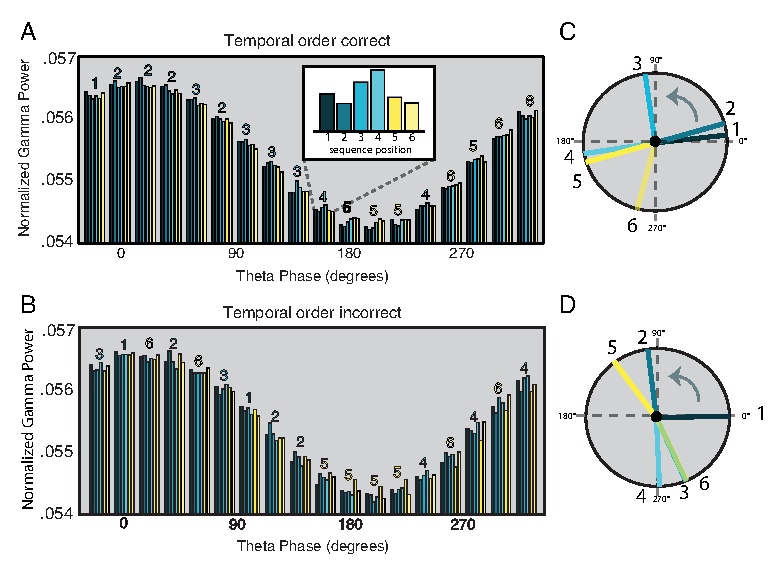
\includegraphics[width=\textwidth]{figures/chapter3_figure2.eps}
  \caption[Phase analysis of theta-gamma coupling by subsequent memory]{Phase analysis of theta-gamma coupling during sequence encoding plotted by position and subsequent temporal order memory for left posterior cluster of sensors.  A.  Theta-binned gamma distributions during successful sequence encoding.  Each color represents a distinct sequence position and the number above the bin represents the sequence position with the highest gamma power at that bin. The inset shows the relative pattern over sequence positions for a single phase bin.  B.  Theta-binned gamma distributions during unsuccessful sequence encoding.  C. Mean angle of theta-gamma coupling for each sequence position for successful sequence encoding.  The main effect (i.e. strong bias of gamma at all positions to the trough of theta) is removed to highlight the relative phase biases.  D. Mean angle of theta-gamma coupling for each sequence position for unsuccessful sequence encoding.}
  \label{chapter3_figure2}
\end{figure}

\subsubsection{Theta phase coding supports temporal sequence
encoding}\label{theta-phase-coding-supports-temporal-sequence-encoding}

While the sensor-level and source-space analyses described above
establish that theta-gamma PAC is modulated by position within a
sequence in a manner that is consistent with the idea that gamma-coded
objects are represented sequentially along the phase of theta, they do
not directly demonstrate that result. Indeed, one could imagine
alternative scenarios where the decreasing theta-gamma PAC pattern
across sequence positions could emerge - a simple example being that the
response pattern represents accumulating item representations without
the orderly representation of their temporal order.

Thus, we conducted additional analyses to directly test our central
hypothesis that objects encountered in different positions within a
sequence are coded at distinct and consecutive phases of theta. To that
end, we first extracted raw MEG data from the two clusters of sensors
that displayed a significant fit to the model derived from our simulated
data (Figure 1d). Separately for these two clusters of sensors, we
binned gamma power by the phase of theta (18 phase bins) to generate an
individual histogram for each trial (during stimulus presentation: 0-2.5
seconds; see Methods for details). We then averaged the theta-binned
gamma distributions for each cluster across all subjects, but separately
for trials in distinct sequence positions and also separately by
subsequent temporal order memory, as we reasoned that phase coding may
be present or robust only during successful sequence encoding.

Examining successfully encoded sequences first, in the left posterior
cluster of sensors we find a main effect of position on the distribution
of gamma power over theta phase (Watson-Williams Test: \emph{F}(5,96) =
16.04, \emph{p} \textless{} .0001) and, critically, the gamma power
distributions reflected the relative order in which the objects were
encoded (Figure 2a; Supplemental Figure 6). By contrast, for sequences
where order memory was later incorrect, we observed significant
differences in mean phase angle by position (Watson-Williams Test:
\emph{F}(5,96) = 5.26, \emph{p} \textless{} .0001), but the order of the
phase angles was scrambled relative to the actual order that the items
were experienced (Figure 2b). Critically, the memory by position
interaction was also significant (Harrison-Kanji Test: \emph{F}(5,196) =
15.79, \emph{p} = .01). Together, these results suggest that objects in
distinct ordinal positions within a sequence may be coded in gamma band
activity biased towards distinct, and ordered, phases of a theta
oscillation.

Another way to visualize this effect is to plot the relative phase
biases in polar coordinates. Thus, we transformed the theta-binned gamma
distributions into polar coordinates, now plotting the mean phase angle
of theta-gamma coupling for each sequence position separately for
sequences where order was later remembered and when they were forgotten,
after removing the main effect of coupling, which was centered at the
trough of theta. We see that, for sequences whose temporal order was
later remembered, the order of the angles across sequence positions
reflected the order in which the objects were encoded (Figure 2c),
whereas for incorrect sequences, the order of the angles is scrambled
relative to the actual encoding order (Figure 2d).

In the next analysis, we averaged the theta-binned gamma distributions
for the 6-sequence positions into 3 bins (1\&2, 3\&4, 5\&6) after
subtracting out the main effect of coupling. A statistical contrast of
each position bin relative to the average of the other two bins shows
that gamma power was preferentially higher at distinct phase bins of
theta (Figure 2c; \emph{t}'s \textgreater{} 2.1, \emph{p}'s \textless{}
.05). However, for sequences where the temporal order was later
incorrectly remembered, the relative distributions for each position bin
were comparatively flat, and there were no single phase bins where the
position bins were significantly different from each other (\emph{t}'s
\textless{} 2.1, \emph{p}'s \textgreater{} .05). Together, these data
are consistent with the idea that successful sequence encoding is
accompanied by a theta-gamma phase coding mechanism, whereby gamma power
associated with each sequential item is biased toward a distinct,
consecutive phase of an underlying theta oscillation.

\begin{figure}
  \centering
  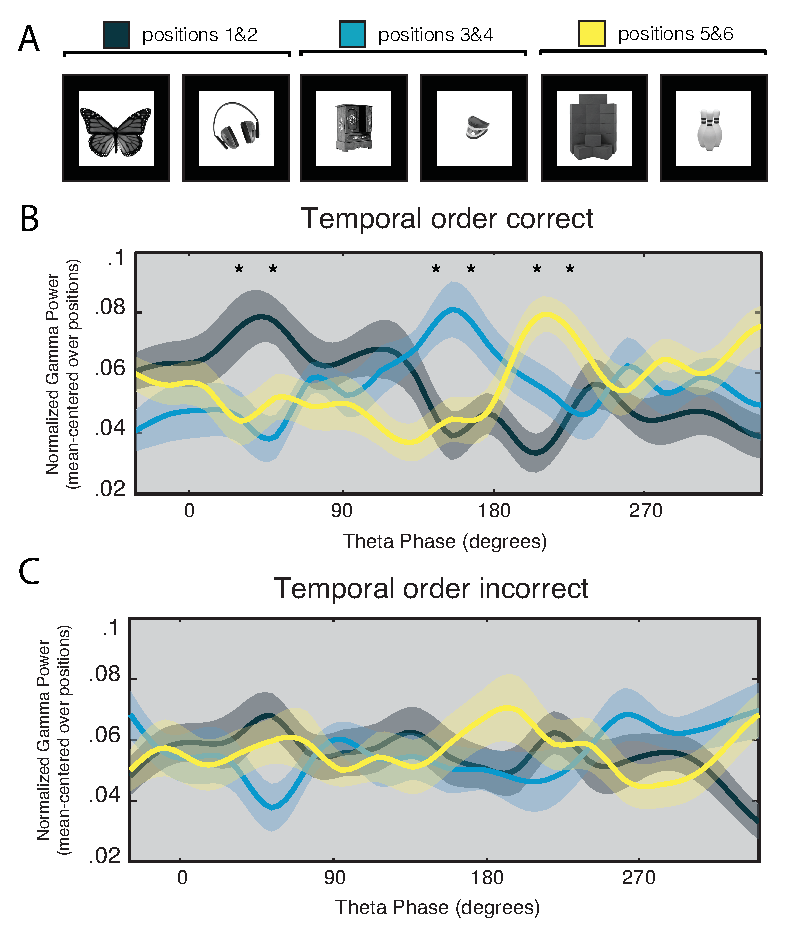
\includegraphics[width=\textwidth]{figures/chapter3_figure3.eps}
  \caption[Relative biases in gamma power over theta phase by sequence position and subsequent memory]{Relative biases in gamma power over theta phase by sequence position and subsequent memory.  A) Schematic representing our binning strategy.  We binned trials into early (1 and 2), middle (3 and 4), and late (5 and 6).  B) The distribution of gamma power over theta phase after removing the main effect of coupling for each sequence bin when temporal order was correct.  C) The same as B, but for sequences where order was incorrect. Stars represent phase bins where the statistical contrast (for example, early vs. the average of middle and late) was significant.  * p<.05}
  \label{chapter3_figure3}
\end{figure}

\subsubsection{Ruling out alternative
explanations}\label{ruling-out-alternative-explanations}

While the results reported here are consistent with a theta phase coding
account of sequence memory formation, it is important to rule out
alternative explanations for the data. Below, we outline a number of
control analyses aimed to test whether other features of the data could
explain the effects.

\emph{Temporal dynamics of gamma power and theta phase locking.} We
considered the possibility that variance in gamma power or theta phase
locking across sequence positions or memory conditions could explain the
phase coding effects. To test this, we analyzed the time course of gamma
power and theta phase locking separately by sequence position (binned
1\&2, 3\&4 and 5\&6) and by subsequent memory in the left posterior
cluster of interest that displayed phase coding. As can be seen in
Supplemental Figure 7 \& 8, transient stimulus-evoked gamma power and
theta phase locking stabilize by 500 ms post stimulus onset. There were
no differences in theta phase locking by position (0-500 ms:
\emph{F}(2,34) = .78, \emph{p} = .46, 500-2500 ms: \emph{F}(2,34) = .5,
\emph{p} = .61{]} and no differences by subsequent memory {[}0-500 ms:
\emph{F}(1,34) = 1.17, \emph{p} = .29; 500-2500 ms: \emph{F}(1,34) =
.04, \emph{p} = .96{]}. Gamma power also did not significantly vary by
sequence position (0-500 ms: \emph{F}(2,34) = .24, \emph{p} = .78;
500-2500ms: \emph{F}(2,34) = .13, \emph{p} = .87) and there was a trend
for greater gamma power in the forgotten sequences compared to the
remembered sequences early (0-500 ms) but not later (500-2500 ms) (0-500
ms: \emph{F}(1,34) = 3.12, \emph{p} = .09; 500-2500 ms: \emph{F}(1,34) =
.95, \emph{p} = .34). It's important to highlight that absolute gamma
power likely did not play a role in the phase coding effects we see
here, because for each trial, after computing the distribution of gamma
power over theta phase, the resulting distribution was normalized (to
sum to 1). This minimizes the likelihood that the phase coding effects
were somehow driven by gamma power differences across conditions.

\emph{Removing the stimulus evoked response.} One major concern when
performing cross-frequency coupling analyses is that the neural response
to the presentation of a stimulus could simultaneously result in a burst
of high-frequency activity and low frequency phase alignment over
trials. Thus, an effect that looks like a phase-amplitude interaction
may actually be driven by two independent processes with a common
driver. It is worth noting that a burst of high-frequency activity at
stimulus onset would need also be accompanied by (1) a predictable shift
in theta phase across each position in a sequence and (2) only do so on
successfully encoded sequences to fully account for our results.
Nonetheless, to rule out the possibility that our effects are in some
way driven by an evoked stimulus response, we reanalyzed the data
without the time window containing the evoked potential.

We then recomputed our phase coding analyses removing the first 500
milliseconds from each trial, which effectively removed the stimulus
onset response from the analysis. We found that both the decreasing PAC
over event positions (Supplemental Figure 9; including first 500ms:
\emph{t}(16) = 6.9868, \emph{p} = 3.0663e-06, excluding first 500ms:
\emph{t}(16) = 6.1015, \emph{p} = 1.5301e-05), as well as the phase
coding by subsequent order memory effects (Supplemental Figure 10;
excluding first 500ms - temporal order correct: Watson William's Test
\emph{F}(5,96) = 9.10, \emph{p} \textless{} .0001; temporal order
incorrect: Watson William's Test \emph{F}(5,96) = 6.42, \emph{p}
\textless{} .001; memory by sequence position interaction:
Harrison-Kanji Test: \emph{F}(5,196) = 11.03, \emph{p} = .025) were
still present and statistically robust.

\emph{Phase coding in the inter-trial interval.} As a further test to
rule out an evoked response confound, we ran these same analyses on the
time periods between each trial, the inter-trial intervals (ITI;
2500-5000 ms post stimulus onset), when participants were presumably
maintaining prior items and reinforcing associations between items.
Interestingly, we found that theta-gamma PAC was in fact stronger during
the ITI than the stimulus presentation interval (see Supplemental Figure
11a) and the phase coding by subsequent memory effects were still
present and robust (temporal order correct: Watson William's Test
\emph{F}(5,96) = 9.10, \emph{p} \textless{} .0001; temporal order
incorrect: Watson William's Test \emph{F}(5,96) = 9.09, \emph{p}
\textless{} .0001; position x memory interaction: Harrison-Kanji Test:
\emph{F}(5,196) = 8.02, \emph{p} = .07). However, the decreasing PAC by
sequence position effect was no longer present (Supplemental Figure
11b). This very intriguing result highlights that phase coding is
persistent even after the stimulus was removed from the screen, thus
ruling out the possibility that the evoked response is in someway
responsible for the phase coding pattern we observed.

\emph{Testing for systematic shifts in theta phase by sequence
position.} Another possible alternative explanation for our result is
that gamma power remains temporally fixed with respect to the onset of
the stimulus, but there is a systematic shift in theta phase as a
function of sequence positions, perhaps due to a reset in the phase of
theta caused by the stimulus presentation. To test for a mechanism of
this nature, we simulated sinusoidal time series at the theta frequency,
where the phase of theta systematically shifted over the sequence, and
then computed the cross-correlation of the simulated time series for
each pair of sequence positions (cross-correlation between 1-2, 1-3,
1-4, etc.). If a systematic theta phase shift is present in the data,
then the peak cross-correlation should also systematically increase with
increasing lag between items. An analysis of this `toy' example
concretized our intuition that the temporal lag of the peak correlation
would increase with distance between sequence positions (Supplemental
Figure 12). We used this framework to test for a systematic phase shift
in our data at the level of each sequence, and then averaging the peak
lag values over sequences and over subjects. We performed this analysis
specifically for correct sequence, as that is where we observed the
phase coding effects. The results do not reveal any evidence for a
systematic theta phase shift across sequences (\emph{F}(4,84) = .33,
\emph{p} \textgreater{} .5; Supplemental Figure 12). Thus, the
phase-amplitude relationship is more likely to be driven by a shift in
gamma across sequence positions rather than a phase shift in theta.

\emph{Testing for systematic changes in theta phase symmetry.} Finally,
another possible explanation for PAC modulation by sequence position is
that the shape of the theta waveform could systematically change,
becoming more or less asymmetric over a sequence of items. While the
exact pattern of expected results would vary based on the phase
dynamics, oscillations with symmetric, sinusoidal phase dynamics will
map to a circular distribution in polar coordinates, while asymmetric
oscillations will map to a non-circular distribution (see Supplemental
Figure 13 for a visualization of this pattern). To test whether an
interaction between phase symmetry and sequence position could explain
these effects, we filtered each trial in the theta band. Then, we
computed group-averaged phase-amplitude distributions in polar
coordinates, averaging separately over each sequence position. The
results suggest that the theta waveforms were equally symmetric over
sequence positions (Watson-Williams test: \emph{F}(5,101) = .23,
\emph{p} = .94), but varied in power, which is evident by increasing
area of the polar phase distributions by sequence position (Supplemental
Figure 13). This replicates the prior finding that theta power
systematically increases over sequence positions. Thus, differences in
phase symmetry are not likely to explain this pattern of results.

\section{Discussion}\label{discussion}

Temporal coding models \autocite{harris_neural_2005} converge on the
idea that the brain may utilize the precise timing of neuronal firing to
encode information. Theta phase coding models
\autocites{lisman_storage_1995}{lisman_-_2013}{lisman_neural_2008}{hasselmo_proposed_2002}{huxter_independent_2003}{tsodyks_population_1996}{dragoi_temporal_2006}
of sequence encoding specifically predict that the order in which a
sequence of events occurred in the external world may be represented
internally in the brain in the timing of neuronal firing (in the gamma
frequency) with respect to the phase of an underlying theta wave. Our
results provide compelling evidence in humans that a bias in gamma power
along the phase of an underlying theta rhythm is apparent during
successful, but not unsuccessful, sequence encoding. These findings
suggest that by associating the ordinal position of a gamma-coded item
representation with a particular theta phase, the brain may preserve the
order in which a sequence occurred.

In this study, we assessed whether gamma power during the encoding of
items in distinct sequence positions was preferentially bias towards
distinct and consecutive phases of theta. Critically, using this
paradigm, we were able to separately examine whether phase coding was
evident during both successful and unsuccessful temporal order encoding
First, consistent with prior research
\autocites{canolty_high_2006}{jacobs_neural_2009}{voytek_shifts_2010}
(but see \textcite{axmacher_cross-frequency_2010}) we found that for all
items (regardless of sequence position), gamma power was maximal at the
trough of the theta cycle. Secondly -- and in line with our primary
predictions -- during sequence encoding, gamma power was shifted
progressively later in the theta cycle for each item in the sequence,
and the relative peak gamma power reflected the order in which the items
were encountered (Figure 2 \& 3). Critically, this ordinal phase coding
effect was only present during sequences participants were later able to
correctly remembered the temporal order of items encountered in that
sequence. The specificity of this effect to successfully encoded
sequences provides strong support for the notion that the brain may code
for recent elements in memory by leveraging relative phase differences
among distinct items in a sequence. The specificity to remembered
sequences also helps to rule out that the effects are somehow derivative
only of the visual and task structure, as the timing of stimulus onset
and task motor responses are the same for trials within sequences where
temporal order was later forgotten and when they were remembered.
Further supporting this point, the memory-related phase coding effects
were present after removing the early trial activity (\textless{}500ms,
during evoked response), and remarkably, even persisted into the
inter-trial interval (when the stimulus is no longer on the screen).
These results provide evidence for a longstanding theory that
theta-gamma phase coding might support temporal sequence memory
\autocite{lisman_-_2013}.

In our initial set of analyses, we found that theta-gamma PAC was
modulated by the position of the object within a sequence. Specifically,
using a computational model-driven linear regression approach (see
Methods), we found that our measure of theta-gamma PAC decreased over
items in a sequence, and this effect was present in left lateralized and
left posterior MEG sensors (Figure 1d). While perhaps counterintuitive,
this decreasing pattern of our PAC measure is predicted by a
computational simulation of our hypothesis (Figure 1c) and is driven by
a broadening of the gamma distribution over a theta cycle (see Figure
2). Then, using an adaptive beamforming technique, the source of this
effect was localized to the left hippocampus, extending into the left
parahippocampal and adjacent fusiform gyri (Figure 1e), consistent with
the suspected role of the left hippocampus and medial temporal lobe
cortex in temporal sequence encoding
\autocites{dubrow_temporal_2014}{hsieh_hippocampal_2014}{jenkins_prefrontal_2010}{tubridy_medial_2011}.

One remaining question is: what is the nature of the mechanism that is
driving the model fits in our initial set of analyses (i.e.~Figure 1d)?
One possibility is that the broadening of gamma power across sequential
positions is the result of the accrual and maintenance of all prior
items within a sequence, each nested in a distinct phase of an
underlying theta oscillation, similar to the model proposed by
\textcite{lisman_storage_1995} and formalized in our computational
simulation (see Figure 1b \& c). It follows then that the representation
of additional items would result in a broader distribution of gamma
power over a theta cycle.\\
A second possibility, however, is that the effect is driven by a
progressive shift in gamma power along the phase of theta while items
are being encoded (in the absence of gamma broadening related to the
accrual of item representations). On its own, this pattern would not
modulate theta-gamma coupling as we measured it. This is because the
measure of coupling we used is sensitive to the width of the gamma
distribution over theta, and a mere shift in gamma power would not
modulate the width of the distribution. However, a forward shift in
gamma power by sequence position -- in conjunction with the strong main
effect of coupling we observed in the data -- could, in fact, account
for the pattern of decreasing PAC by sequence position that we observed.
For instance, if items in early sequence positions were preferentially
locked to the trough of theta (i.e.~where gamma power is highest for all
sequence positions in our data), this pattern would result in an
exaggerated measure of theta-gamma coupling for early positions. If
items later in a sequence were preferentially coded at the theta power
peak (i.e.~where gamma is lowest for all sequence positions), this would
result in an attenuated measure of theta gamma coupling. While a subtle
(but very important) point, our initial analyses were actually agnostic
to the relative likelihood of either of these two possibilities.

Our data are more consistent with the latter model where a
position-related forward shift in gamma power along the phase of theta
supports sequence memory encoding, in the absence of accruing
gamma-coded item representations. There are two major data points that
led us to this conclusion. First, if additional items are being added
into the sequence representation, one might expect overall measures of
gamma power to increase across the sequence as well. Contrary to this
expectation, gamma power was relatively flat across the sequence
(Supplemental Figure 3). Secondly, one might also expect, that the width
of the gamma power distribution over theta should broaden as a function
of sequence position (as more item representations are accrued and
maintained). Contrary to this hypothesis, we did not see evidence that
the width (standard deviation) of the distribution increased across
sequence positions (\emph{F}(1,15) = .20, \emph{p} \textgreater{} .5).
Thus, we believe that the best explanation for our results is that
sequence encoding is supported by a temporal shifting of gamma power
(representing each item) along the phase of an underlying theta
oscillation.

With this conclusion in mind, it is important to point out that in order
to examine gamma power associated with each sequential position, we had
to examine a time window that was actually associated with each item
presentation -- i.e.~the time period when that stimulus was presented,
as well as the immediately following inter-trial interval. In its
original conception, the Lisman and Idiart model was proposed as a
mechanism to support the maintenance of multi-item sequences in working
memory - after items had been encountered and were presumably being
actively maintained. We reasoned if gamma power associated with each
item representation in a sequence is ordered along an underlying theta
wave, we should be able to measure this effect while these items are
being encoded. Thus, the current results do not preclude the possibility
that, during working memory, if one could track the gamma power
associated with each item into subsequent time periods, that they would
still be associated with the same phase of theta.

Furthermore, the maintenance of multiple items is likely to be dependent
on the task and specifically whether items are being `actively' retained
in working memory. Our task is not necessarily an `active' working
memory task in the sense that participants are not required to rehearse
and maintain the sequence of items during a delay period as in classical
working memory paradigms. Rather, participants are instructed to
remember the temporal order of the sequence by forming associative links
between neighboring items, which likely involves some working memory
maintenance along with other associative encoding operations. Thus, our
current results are agnostic as to whether one would see the continued
maintenance of phase coding effects during working memory rehearsal.
Thus, it is important to point out that this data is not necessarily in
conflict with the Lisman and Idiart model, and may in fact be
parsimonious. Future studies should test whether there is a relationship
between theta-gamma phase coding during sequence memory encoding and
theta/gamma activity that has been observed during working memory
maintenance \autocite{axmacher_cross-frequency_2010}.

The gamma power effects we report here peaked between
\textasciitilde{}70-100 Hz. Critically, recent work using simultaneous
MEG/iEEG suggests that gamma power \textless{}100 Hz is reliably
detectable \autocite{dalal_simultaneous_2013}. Interestingly, recent
work in rodents suggests that there is a functional distinction between
high (\textasciitilde{}60-100 Hz) and low (25-55 Hz) gamma in the
hippocampal circuit, such that lower frequency theta-locked gamma
`sweeps' may represent the future spatiotemporal trajectory of the
animal, while fast theta-locked gamma may support the coding of ongoing
trajectories in real-time \autocite{zheng_spatial_2016}. Possibly
related to this dissociation, in the current study, where subjects were
encoding trial-unique sequences (i.e.~sequences did not repeat, and thus
could not be `predicted'), we observed our memory-related phase coding
effects in high gamma. Future work could test whether a theta phase --
low gamma power relationship emerges with repeated sequences, possibly
indexing the forward prediction of upcoming items. While its important
to note that our experimental design as well as the signals that we are
recording are admittedly very different than the rodent study discussed
above, it is nonetheless intriguing to consider parallels between the
datasets.

While gamma power was relatively stable over positions, we observed an
increase in theta power across the sequence. This is consistent with
studies that show theta power increases during memory encoding
\autocites{summerfield_coherent_2005}{sederberg_theta_2003} and working
memory maintenance
\autocites{hsieh_neural_2011}{gevins_high-resolution_1997}{raghavachari_gating_2001}{scheeringa_trial-by-trial_2009}.
A prior study observed theta power increases specifically during delay
period maintenance of temporal order information as compared to the
maintenance of just the items themselves \autocite{hsieh_neural_2011}.
One possibility is that theta power increases reflect control processes
related to relational encoding
\autocites{hsieh_neural_2011}{summerfield_coherent_2005}. Consistent
with this idea, we see that sustained theta power increases occur
predominantly over frontal regions (see Supplemental Figure 1), possibly
reflecting prefrontal control processes involved in representing
temporal relations among items \autocite{blumenfeld_putting_2011}.

There is a rapidly growing literature linking theta-gamma coupling to
human memory
\autocites{canolty_high_2006}{axmacher_cross-frequency_2010}{mormann_phase/amplitude_2005}{fuentemilla_theta-coupled_2010}{maris_spatially_2011}{friese_successful_2013}{lisman_-_2013}
, and to cognition more generally. These memory studies all converge on
the idea that theta-gamma phase-amplitude coupling plays a role in the
maintenance, as well as the long-term retention of mnemonic information.
While these prior studies have been critical to advancing our
understanding of the temporal dynamics of episodic memory formation, the
fundamental and important question of whether theta phase coding
supports sequence encoding has not been tested. To our knowledge, these
data provide the first empirical evidence in humans that memory for
sequences of information is supported by the precise timing of
item-related gamma activity with respect to an underlying theta
oscillation.

Prior work in rodents has leveraged the spatial specificity of `place
cells' \autocites{okeefe_hippocampus_1971}{okeefe_review_1979} to show
that sequences of hippocampal place cells representing a `movement
trajectory' not only fire during an experience, but also later `replay'
in a similar order on subsequent cycles of a theta oscillation
\autocites{gupta_segmentation_2012}{johnson_neural_2007}{wikenheiser_hippocampal_2015}{foster_hippocampal_2007}{pastalkova_internally_2008}{dragoi_temporal_2006}.
The current result, by analogy, demonstrates that the encoding of an
episodic `object trajectory' or temporal sequence of items is also
supported by a theta phase code. Given these two sets of findings, it is
possible that the sequential coding of information along the phase of a
theta oscillation represents an all-purpose mechanism in the brain that
allows for temporally or spatially separated information to be
associated via long-term potentiation. In summary, these results fill a
critical gap in the literature by providing new empirical evidence from
a well-controlled and characterized behavioral paradigm in humans that
theta-gamma phase-amplitude coupling and more specifically, theta phase
coding, supports object sequence memory.

\section{Supplemental Figures}\label{supplemental-figures}

\begin{figure}
  \centering
  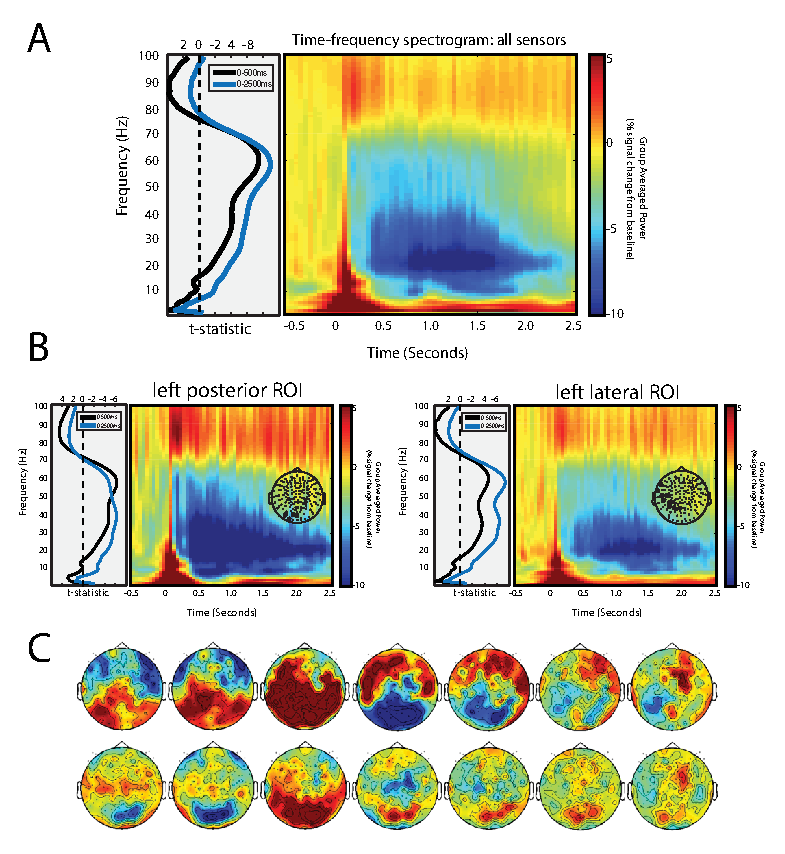
\includegraphics[width=.75\textwidth]{figures/chapter3_suppfigure1.eps}
  \caption[Time-frequency power during stimulus presentation]{\textit{Time-frequency power during stimulus presentation.} (A) Average time-frequency spectrogram is plotted across all sensors and all subjects, where 0 represents stimulus onset.  Power is calculated relative to a pre-stimulus baseline (-1 to -.5).  The line plots on the left side are group-level t-values representing the statistical contrast of the stimulus on period versus the pre-stimulus baseline. The black line represents 0-500ms and the blue line represents 0-2500ms (i.e. the duration of the stimulus on period). (B) Time-frequency power is plotted specifically for the two clusters of sensors that showed the pattern of decreasing theta-gamma coupling by sequence position.  (C) Topographic plots in time bins of 500ms during stimulus presentation.  The top row is theta power and the bottom row is gamma power. }
  \label{chapter3_suppfigure1}
\end{figure}

\begin{figure}
  \centering
  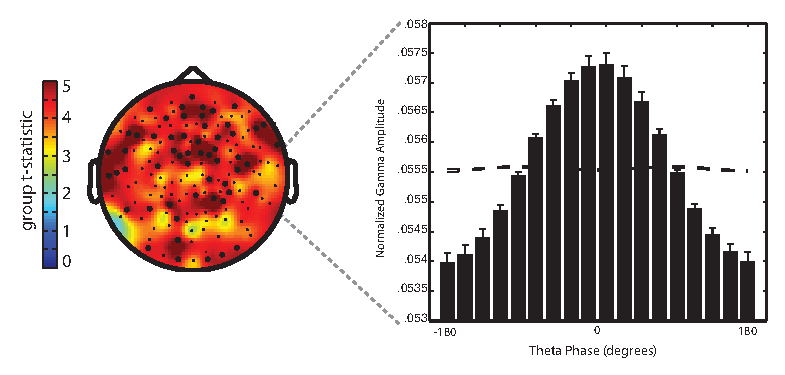
\includegraphics[width=\textwidth]{figures/chapter3_suppfigure2.eps}
  \caption[Theta-gamma coupling across all sensors]{\textit{Theta-gamma coupling across all sensors.} (Left) Topographic plot of group-level t-statistics representing sensors that showed significant theta-gamma coupling during the sequence encoding task (0-2.5 seconds; t(16)>3.96, p<.001).  Filled circles on the topographic plot represent significant sensors. (Right) Gamma power binned by theta phase for sensors that showed significant theta-gamma coupling.  Error bars represent standard error of the group mean.  The dotted lines represent the standard error of the mean of the permuted coupling scores (see Methods for details).}
  \label{chapter3_suppfigure2}
\end{figure}

\begin{figure}
  \centering
  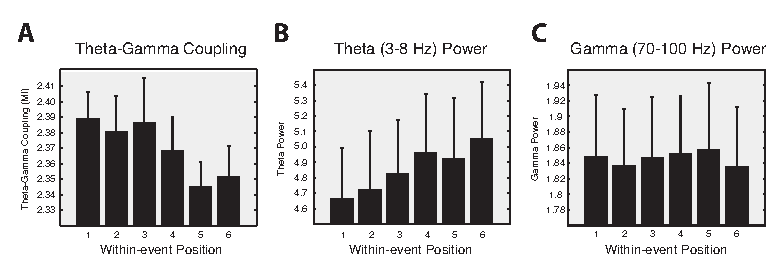
\includegraphics[width=\textwidth]{figures/chapter3_suppfigure3.eps}
  \caption[Power and coupling averaged across significant clusters of sensors]{\textit{Power and coupling averaged across significant clusters of sensors.} (A) Bar graph representing magnitude of theta-gamma coupling (MI or ‘modulation index’) by sequence position averaged across sensors that displayed a significant fit to theta-gamma model.  (B) Theta power by sequence position averaged across sensors displaying significant fit to theta-gamma model. (C) Gamma power by sequence position averaged across sensors displaying significant fit to theta-gamma model.  Error bars represent standard error of the mean.}
  \label{chapter3_suppfigure3}
\end{figure}

\begin{figure}
  \centering
  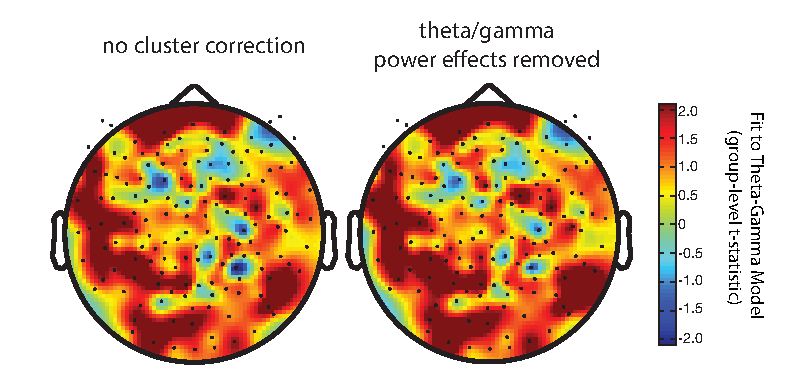
\includegraphics[width=\textwidth]{figures/chapter3_suppfigure4.eps}
  \caption[Decreasing theta-gamma PAC by sequence position model fit data and control analyses]{\textit{Decreasing theta-gamma PAC by sequence position model fit data and control analyses.} The left topographic plot is a statistical plot representing the fit of the theta-gamma model prediction to the theta-gamma coupling data prior to applying the cluster threshold (i.e. Figure 1d before cluster correction, See Methods for details of cluster size permutation procedure).  The right topographic plot represents the result of an analysis where power effects in the theta and gamma band were first regressed out of the theta-gamma coupling data and then the residuals of this analysis were fit to the predicted pattern from the theta-gamma model.}
  \label{chapter3_suppfigure4}
\end{figure}

\begin{figure}
  \centering
  \includegraphics[width=.75\textwidth]{figures/chapter3_suppfigure5.eps}
  \caption[Source localization analysis with various statistical thresholds]{\textit{Source localization analysis with various statistical thresholds.} The statistical maps represent the group-level fit of the decreasing PAC by sequence position model to the theta-gamma coupling data at various thresholds (p<.001, .01 .1, all uncorrected).  Coronal slices are on the top row, axial slices in the middle row, and sagittal slices are along the bottom row.}
  \label{chapter3_suppfigure5}
\end{figure}

\begin{figure}
  \centering
  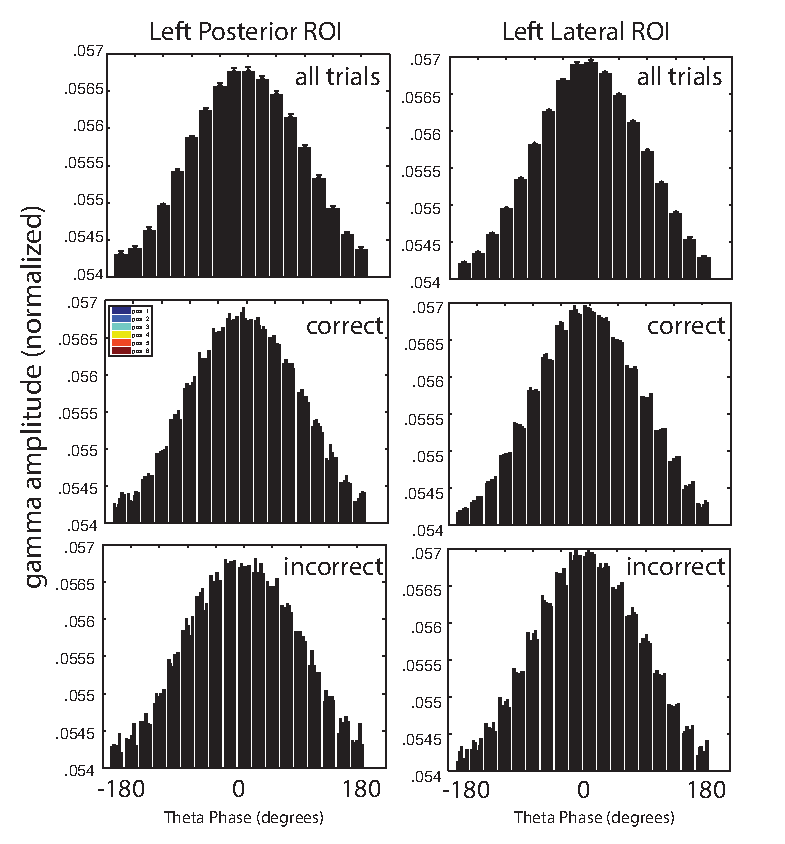
\includegraphics[width=.75\textwidth]{figures/chapter3_suppfigure6.eps}
  \caption[Group-averaged gamma power binned by theta phase for regions of interest]{\textit{Group-averaged gamma power binned by theta phase for regions of interest.} The two clusters of sensors that showed a significant fit to the decreasing theta-gamma PAC by sequence position model.  On the left, data was extracted from the left posterior cluster of sensors that significantly fit the model of decreasing phase amplitude coupling.  On the top is the group-average across all trials (i.e. irrespective of sequence position).  In the middle, theta-gamma coupling is plotted as a function of sequence position only for trials where the order was later correct and on the bottom, only for trials where the order was later incorrect.  The plots on the right are the same as the left, but for the left lateral cluster of interest.}
  \label{chapter3_suppfigure6}
\end{figure}

\begin{figure}
  \centering
  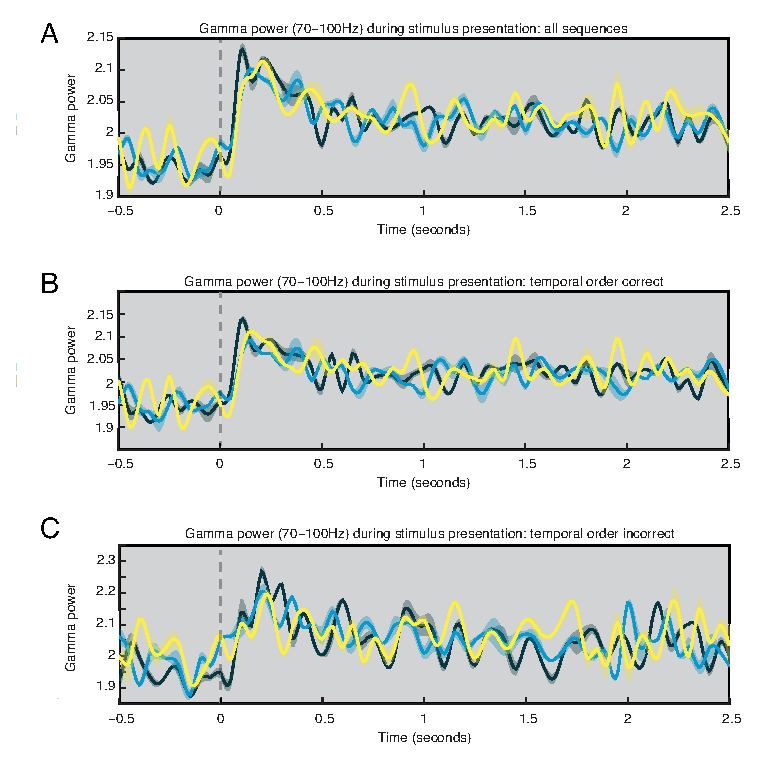
\includegraphics[width=\textwidth]{figures/chapter3_suppfigure7.eps}
  \caption[Gamma power during stimulus presentation]{\textit{Gamma power (70-100 Hz) during stimulus presentation.} (A) Group-averaged time course of gamma power (-.5 to 2.5 seconds) in left posterior cluster of interest for early (dark gray; sequence positions 1 and 2), middle (blue; 3 and 4) and later (yellow; 5 and 6) sequence positions. B) Same as A but for only correctly remembered sequences. (C) Same as A but only for incorrect sequences.  Error bars represent standard error of the mean.}
  \label{chapter3_suppfigure7}
\end{figure}

\begin{figure}
  \centering
  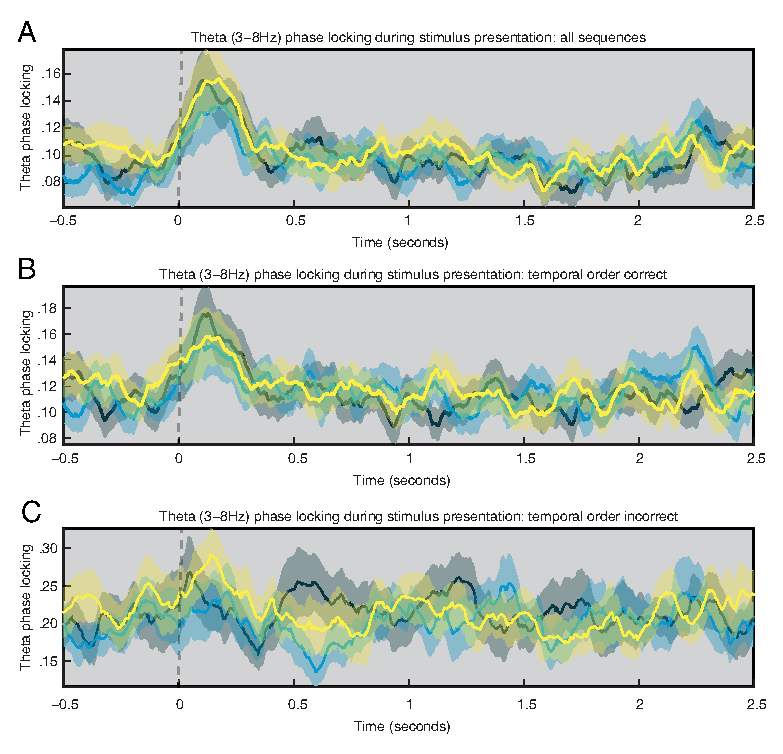
\includegraphics[width=\textwidth]{figures/chapter3_suppfigure8.eps}
  \caption[Theta phase locking during stimulus presentation.]{\textit{Theta phase locking (3-8 Hz) during stimulus presentation.} (A) Group-averaged time course of theta phase locking (-.5 to 2.5 seconds) in left posterior cluster of interest for early (dark gray; sequence positions 1 and 2), middle (blue; 3 and 4) and later (yellow; 5 and 6) sequence positions. (B) Same as A but for only correctly remembered sequences. (C) Same as A but only for incorrect sequences.  Error bars represent standard error of the mean.}
  \label{chapter3_suppfigure8}
\end{figure}

\begin{figure}
  \centering
  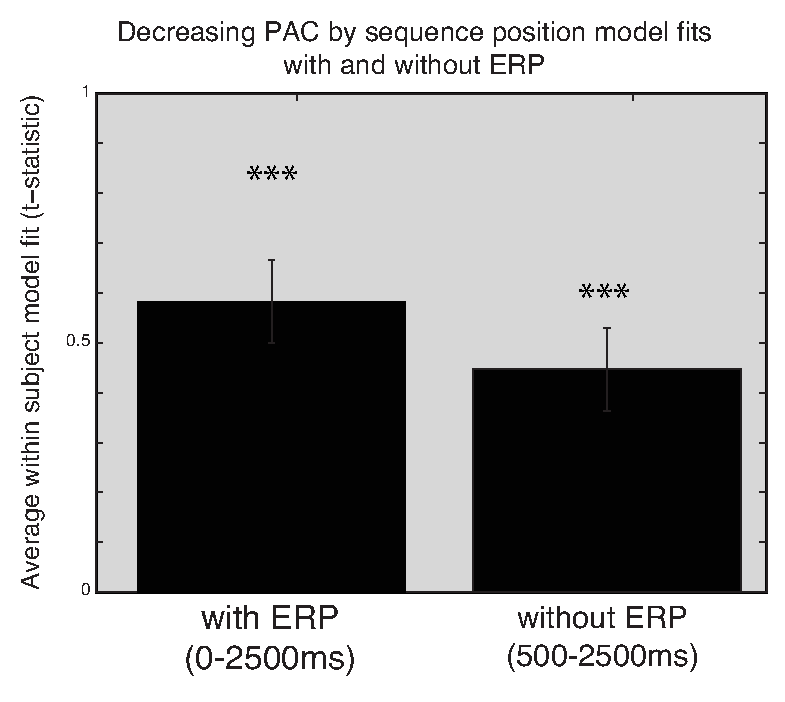
\includegraphics[width=.75\textwidth]{figures/chapter3_suppfigure9.eps}
  \caption[Model fit without ERP]{\textit{Model fit without ERP.} This bar graph depicts the average model fit statistic for a linear decrease in theta-gamma PAC by sequence position, averaging over sensors that showed a significant group-level model fit.  The bar on the left represents the average model fit for the original analysis on the entire stimulus presentation (0-2500ms).  The bar on the right represents the average model fit for the new analysis where we remove the first 500ms (500-2500ms), eliminating the possible contribution of the evoked response.  *** p<.001.}
  \label{chapter3_suppfigure9}
\end{figure}

\begin{figure}
  \centering
  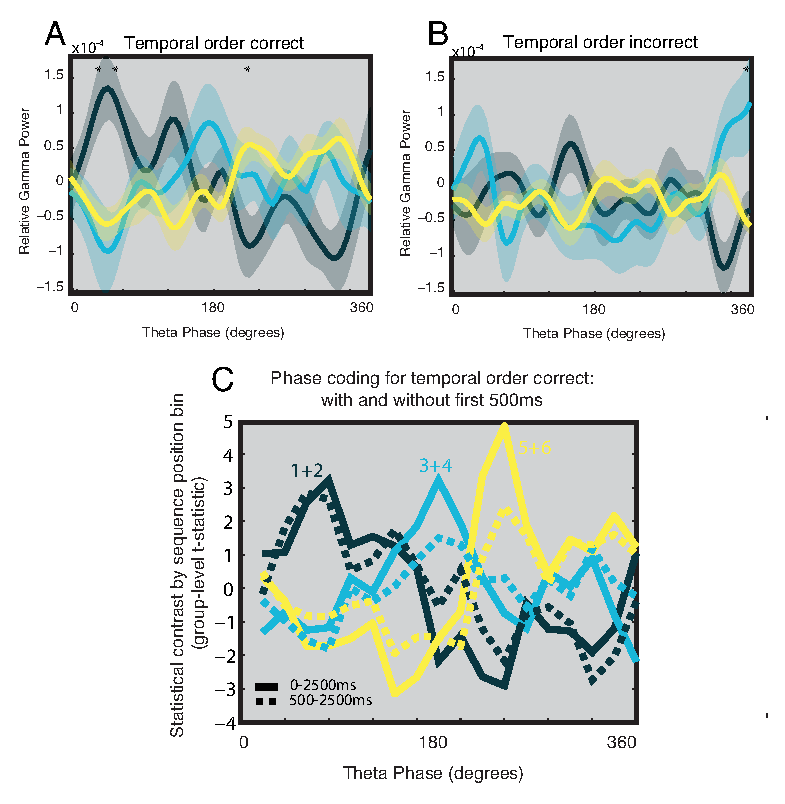
\includegraphics[width=\textwidth]{figures/chapter3_suppfigure10.eps}
  \caption[Phase coding plots without ERP]{\textit{Phase coding plots without ERP.}  Distribution of gamma power over theta phase by sequence position bin for only correctly remembered sequences (Watson William’s Test F(5,96)=9.10, p<.0001). B) Distribution of gamma power over theta phase by sequence position bin for incorrectly remembered sequences (Watson William’s Test F(5,96)=6.42, p<.001). Sequence by position interaction is significant (Harrison-Kanji Test: F(5,196)=11.03, p=.025). C) Group-level statistics for theta phase coding effect with (solid line) and without first 500ms (dashed line). p<.05}
  \label{chapter3_suppfigure10}
\end{figure}

\begin{figure}
  \centering
  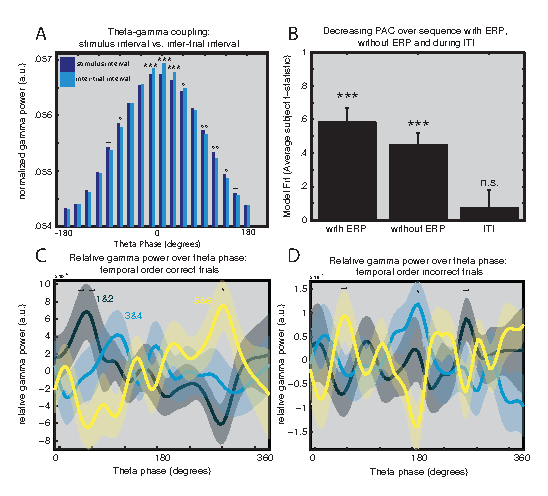
\includegraphics[width=\textwidth]{figures/chapter3_suppfigure11.eps}
  \caption[Theta-gamma coupling during inter-trial interval]{\textit{Theta-gamma coupling during inter-trial interval (ITI; 2500-5000 post stimulus duration).} Histogram of gamma power over theta phase for the stimulus presentation interval (dark blue) and the ITI (light blue). (B) Decreasing PAC by sequence position model fits during the entire stimulus interval, after removing the first 500ms and during the ITI. (C) Distribution of gamma power over theta by sequence position for correct order sequences during the ITI (Watson William’s Test F(5,96)=9.10, p<.0001). (D) Distribution of gamma power over theta by sequence position for incorrect sequences during the ITI (Test F(5,96)=9.09, p<.0001). Sequence by position interaction trending (F(5,196)=8.02, p=.07). ~ p<.1, * p<.05, ** p<.01, *** p<.001.}
  \label{chapter3_suppfigure11}
\end{figure}

\begin{figure}
  \centering
  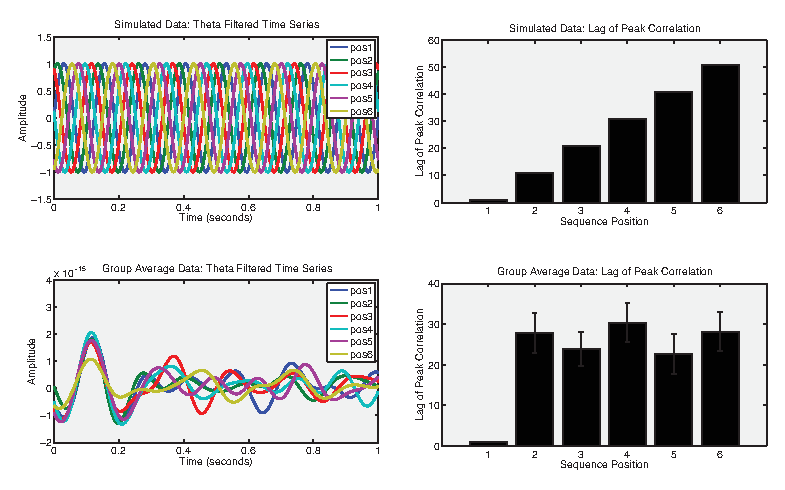
\includegraphics[width=\textwidth]{figures/chapter3_suppfigure12.eps}
  \caption[Testing for systematic theta phase shift by sequence position.]{\textit{Testing for systematic theta phase shift by sequence position.} The top row is simulated data in the theta frequency for each sequence position, where we simulated a systematic linear phase shift over the sequence.  The bottom row is the group-averaged data after computing each of these metrics within-subject.  The left column is the data filtered in the theta band. The right row is the lag of the peak in the pair-wise cross-correlation.  If a systematic phase shift was present in the data, we would expect a monotonically increasing lag as a function of sequence position.}
  \label{chapter3_suppfigure12}
\end{figure}

\begin{figure}
  \centering
  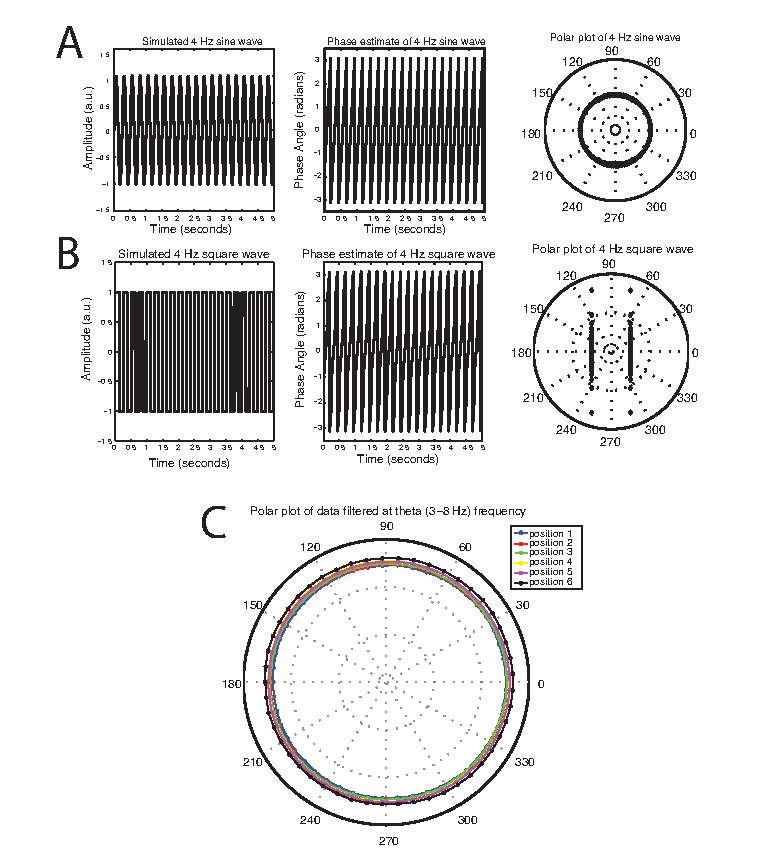
\includegraphics[width=.75\textwidth]{figures/chapter3_suppfigure13.eps}
  \caption[Theta phase symmetry]{\textit{Theta (3-8 Hz) is symmetric and symmetry doesn’t vary by sequence position.} (A) On the left is a simulated 4 Hz sine wave.  Plotted in the middle is the phase time series of the theta wave.  On the right, the waveform is plotted in polar coordinates, where the circular angle represents the phase and the distance from the center represents the power. (B) The same plot as listed above, but for a square wave at 4 Hz. (C) Polar plot representing the grand average of the MEG time series during stimulus presentation (0 to 2.5s) filtered in the theta range (3-8 Hz) and averaged over the left posterior cluster of sensors.  Each color represents a distinct sequence position.}
  \label{chapter3_suppfigure13}
\end{figure}


\begin{conclusion}
\input{conclusion}
\end{conclusion}

\input{appendix}
\addcontentsline{toc}{chapter}{Bibliography}

\printbibliography


\end{document}
